\documentclass[11pt]{article}
\usepackage{geometry,booktabs,siunitx,tabularx,ragged2e,booktabs,caption}
\usepackage[T1]{fontenc}
\usepackage[utf8]{inputenc}
\newcolumntype{C}[1]{>{\Centering}m{#1}}
\renewcommand\tabularxcolumn[1]{C{#1}}
\usepackage[english]{babel}
\usepackage{natbib,bookmark,hyperref,float,etoc,graphicx,doi}
\graphicspath{{./figures/}} 
\usepackage{epstopdf}
\epstopdfsetup{outdir=./}
\usepackage{xcolor}

\hypersetup{
    colorlinks,
    linkcolor={blue},
    citecolor={blue},
    urlcolor={blue}
}

\urlstyle{same}
%\bibliographystyle{econometrica} 
%use plainnat for WP because then the URLs and DOIs show up as links. 
\bibliographystyle{plainnat} 
\usepackage{amssymb,amsfonts,amsthm,amsmath,latexsym,amstext}
\linespread{1.2}
%\setlength{\parskip}{0.5em} 
\theoremstyle{plain} 
\newtheorem{thm}{Theorem}[section]
\newtheorem{conj}{Conjecture}[section]
\newtheorem{lemma}[thm]{Lemma}
\newtheorem{prop}[thm]{Proposition}
\newtheorem{corl}[thm]{Corollary}
\newtheorem{defn}{Definition}[section]
\newtheorem{exmp}{Example}[section]
\newtheorem{assump}{Assumption}[section]
\newtheorem{rmk}{Remark}[section]

%following are the parameters used in the examples. 
\newcommand{\alphval}{0.33}
\newcommand{\sig}{0.2}
\newcommand{\lbar}{0.5}
\newcommand{\mulow}{0.0}
\newcommand{\muhigh}{0.06}
\newcommand{\rhoD}{0.04}
\newcommand{\rhoS}{0.02}
\newcommand{\rhoval}{0.06}


\begin{document}

\title{The Optimal Taxation of Business Owners}
\date{\today} 
\author{Thomas Phelan\thanks{This is a revised version of the first chapter of my Ph.D. dissertation completed at the University of Minnesota and previously circulated as, "On the efficient level of inequality in business income." I have benefited from discussions with Brian Albrecht, Hengjie Ai, Anmol Bhandari, V.V. Chari, Sebastian Di Tella, Sergio Ocampo, Chris Phelan, Guillaume Sublet, and seminar participants at various conferences. Replication files may be found at \href{https://github.com/tphelanECON/Optimal_taxation_business_owners}{https://github.com/tphelanECON/Optimal\_taxation\_business\_owners}. All remaining errors are of course my own.} \\ Federal Reserve Bank of Cleveland}



\maketitle

\begin{abstract} 
Business owners in the United States are disproportionately represented among the wealthy and are exposed to substantial idiosyncratic risk. Further, recent evidence indicates that business income primarily reflects returns to the human capital of the owner. Motivated by these facts, this paper characterizes stationary efficient allocations and signaling equilibria with linear taxes when business income depends on innate ability, luck, and the past effort of the owner. I first show that in stationary efficient allocations, more productive entrepreneurs typically bear more risk and the distributions of consumption and firm size are approximately Pareto, with the tail of the latter typically thicker than that of the former. I then consider allocations in which entrepreneurs may save in a risk-free bond and signal a willingness to exert continued effort by retaining a fraction of their wealth in their firm. The optimal linear taxation policy calls for separate treatment of firm profits, interest, and wealth. The tax on profits plays a redistributive role, the tax on interest affects the incentives to retain equity and exert effort, and the tax on wealth affects the degree of consumption smoothing over time.  

\smallskip

\textbf{Keywords}: Optimal taxation, moral hazard, optimal contracting.

\smallskip

\textbf{JEL Codes:} D61, D63, E62.

\end{abstract}


\iffalse

Change capital income to interest income. 

\fi

\newpage

\section{Introduction} \label{intro}


It is well-known that the distributions of income and wealth in the United States are skewed to the right and have become more unequal in recent decades. What is perhaps less well-known is that much of this increase is due to the growing importance of business income. \cite{smith_capitalists_2019} and \cite{cooper_business_2016} document that business income now accounts for a greater share of the top 0.1 percent of income than both non business capital income and wage income. Further, \cite{smith_capitalists_2019} also show that business income depends on the owners' active participation by documenting that the death of an owner on average leads to profits falling by more than half.\footnote{See page 1878 of \cite{smith_capitalists_2019}.}

% show that for owners earning more than \$1 million the average fall in profits is 82 percent, while in an \href{https://www.econstor.eu/bitstream/10419/262673/1/wp271.pdf}{earlier} version without this last qualifier, the average fall is 54 percent.

The appropriate policy response to these facts naturally depends on their underlying causes, and in particular, whether business income reflects innate ability, current effort, or past investments. For instance, if income were risk-free and business income solely represented the return on savings, then the results of \cite{chamley_optimal_1986} and \cite{judd_redistributive_1985} imply that business income ought not to be taxed at all, at least in the long run. If instead business income depended solely on exogenous productivity and the current choice of hours worked as in \cite{mirrlees_exploration_1971}, then as \cite{diamond_case_2011} show, the top marginal tax rate may well be over 70 percent. However, both of these approaches miss something important about the above facts. If business income were solely the return to savings then the owner ought not to matter, and if productivity were unaffected by policy and owner actions it is not clear why its distribution should vary across time. Further, neither of the above views provides guidance on whether we ought to levy different taxes on profits, interest income, or capital gains. 


Motivated by these considerations, this paper characterizes stationary efficient allocations and signaling equilibria with linear taxes in an environment in which business income is risky, grows over time, and depends on the past (unobserved) effort exerted by the owner. I first adopt a mechanism design approach and consider the problem of a planner who may choose any allocation which satisfies the constraints imposed by asymmetric information. I then use the insights obtained from this abstract framework to sharply characterize optimal linear taxes in an environment in which entrepreneurs signal a willingness to exert unobservable effort by promising to retain a fraction of their wealth in their firm. 

In order to characterize constrained-efficient allocations, I first alter the principal-agent model of \cite{sannikov_continuous-time_2008} to incorporate persistent effects of effort on output. I assume that the output of a firm at any moment is publicly observable and independent of current choices, but that the growth of its output over time is stochastic and depends on the owner's effort. To induce the owner to exert high effort, high realizations of output growth must be followed by either high consumption or leisure, leading to imperfect risk-sharing and inequality in all efficient allocations. For standard preferences, it becomes increasingly expensive to motivate agents with histories of high growth. When the expected return to effort is fixed over time as in \cite{sannikov_continuous-time_2008}, the principal therefore rewards rich agents with leisure (instead of only consumption) and such agents bear little to no risk. In contrast, the dependence of growth on effort in this paper implies that the return to effort is increasing in firm size, which has important implications for both the dynamics of risk-sharing and its distribution across income levels. Although it is still true that the cost of motivating agents rises with their consumption, in the efficient allocation of this paper agents typically obtain high consumption precisely because their productivity rose, and so the benefits of inducing effort rise along with the costs. 
 
After characterizing the optimal contract, I show how the problem of a planner facing an economy with entrepreneurs and workers decomposes into a series of problems identical in form to a principal-agent problem. The persistent effect of effort has important implications for the implied stationary distributions of consumption and firm size, where is the latter is measured either by output or employment. In contrast with \cite{sannikov_continuous-time_2008}, in which rich agents bear no risk and consumption is bounded above, the distribution of consumption in the stationary efficient allocations of this paper is approximately Pareto in the right tail. Further, when I restrict effort to be fixed over time, the stationary distributions of both consumption and firm size are double Pareto with tail parameters that in general differ from one another. These ``restricted-action'' allocations, the optimal allocations attainable with constant effort, are both simple to characterize and provide intuition for the tail of the efficient allocation because the welfare loss of assuming the highest effort indefinitely vanishes as productivity rises. 

%Intuitively, 

Following this characterization I consider the implications for taxation policy. Prescriptions for taxes unavoidably depend on the degree of risk-sharing present in private markets and contracts that agents are capable of signing. At one extreme, if agents may write contracts of arbitrary complexity with financial intermediaries, then the optimal policy calls only for lump-sum transfers between agents at birth, because the government has no advantage over the private sector at overcoming agency frictions. However, since the assumption of such contracts may be unrealistic, to complement the above I characterize the optimal linear taxes on profits, capital income and wealth in an environment in which agents may save in a risk-free bond and trade shares in their firms. 

I consider equilibria of a signaling type, in which each entrepreneur announces at the initial date a fraction of their wealth that they will retain in their business in perpetuity, and at subsequent periods make consumption-savings and (unobservable) effort choices. The price per share of the firm depends on the beliefs of outside investors over the owner's effort, and the equilibrium notion imposes the requirement that these beliefs are true in equilibrium, given the incentives of the owner. Although the class of linear taxes does not, in general, implement the stationary constrained-efficient allocation, this optimal taxation exercise draws upon a parsimonious characterization of the class of constant effort allocations to obtain novel insights in an environment with heterogeneous agents and endogenous productivity. Further, the welfare loss from adhering to linear taxes becomes arbitrarily small as the number of workers per entrepreneur grows large, and the optimal equilibrium allocation approaches the constrained-efficient allocation. 


The dependence of productivity on unobserved effort implies an important effect of taxation policy in the presence of active equity markets: taxes on interest affect the incentives for outside investors to purchase shares in a business and hence affect the degree of risk-sharing in the private sector. Intuitively, the willingness of investors to purchase shares in a firm will depend on the incentives of the owner to exert continued effort to improve productivity, and hence on the fraction of their wealth invested in the firm. This in turn depends upon the outside option available to the owner, the return on risk-free savings, which is endogenous to taxation policy. These taxation results are reminiscent of \cite{albanesi_optimal_2006}, who shows that the need to provide incentives for effort can justify the double taxation of capital income in a two-period model in which physical capital is exogenously distributed equally across entrepreneurs. In contrast with \cite{albanesi_optimal_2006}, I allow firm size to be endogenous to tax policy, grow over time and to depend on the entire history of the owner's effort. The dependence of output on the owner's productivity ensures that unlike the case of physical capital, it is simply not feasible to reallocate all factors of production across agents. Consequently, in both the efficient and equilibrium allocations in this paper, even arbitrarily successful entrepreneurs remain exposed to the output of their firm and continue to exert effort to improve productivity, as only they are capable of doing so. 

%Put simply, if an entrepreneur's talent 

Under the above assumptions, the optimal stationary equilibrium with linear taxes calls for different taxes on profits, interest, and wealth, playing conceptually distinct roles. The redistributive role is played by the profits tax, as this effectively taxes the inelastic quantity of the model: the endowed ability of the firm owner. The profits tax reduces the ex-ante value of the firm, but has no effect on the subsequent incentives to save or issue shares throughout the agent's life. In contrast, taxes on interest income and wealth alter the private return to effort in one's business and consumption smoothing, respectively. Further, whether or not the taxes on interest and wealth raise any revenue depends crucially on the nature of preferences. In particular, in the case of logarithmic utility, consumption is a martingale in the optimal competitive equilibrium and the taxes on interest income and wealth raise no revenue in the aggregate. 

%admits a simple closed-form expression in terms of 


\textbf{Related literature.} A vast literature builds upon \cite{mirrlees_exploration_1971} to derive optimal taxes in economies with asymmetric information. \cite{scheuer_entrepreneurial_2014} considers entrepreneurs and firm formation and allows for pecuniary externalities across occupations and the possibility of occupation-specific taxation. \cite{ales_taxing_2017} adopt a span-of-control technology as in \cite{rosen_authority_1982} and \cite{lucas_size_1978} and allow firm size to be endogenous. \cite{scheuer_taxation_2017} study optimal taxation policy in the presence of ``superstar'' effects in the form of assortative matching between individuals and firms, and \cite{ales_taxing_2016} consider a similar environment in which the planner has an explicit concern for the welfare of shareholders. Although the above models incorporate business income, they are static and so no agent bears risk or is subject to a moral hazard problem. 

The study of dynamic extensions of \cite{mirrlees_exploration_1971} begins with \cite{golosov_optimal_2003}, and is often referred to as the New Dynamic Public Finance. Most papers within this literature, such as \cite{golosov_redistribution_2016} and \cite{farhi_insurance_2013}, focus on the properties of optimal taxes with exogenously evolving wages. \cite{stantcheva_optimal_2017} considers an extension of this framework in which wages depend on both exogenous ability and the stock of human capital, but there is no moral hazard and no agent employs workers or trades shares in his business. Closer to the current paper are \cite{albanesi_optimal_2006}, \cite{kapicka_optimal_2019} and \cite{best_optimal_2012}, who conduct optimal taxation exercises in two-period economies with hidden effort, and \cite{makris_taxation_2021}, who conduct a similar analysis in an environment with learning-by-doing. However, these papers do not derive implications for long-run distributions of consumption or income, and because their two-period nature cannot address how the risk borne by any agent depends on his history of productivity.\footnote{\cite{makris_taxation_2021} calibrate their model to the average working life span in the US, but the productivity of agents only changes once and so the dynamics are identical to a two-period model.} 


An older literature within public finance, surveyed in \cite{chari_optimal_1999} and often termed the ``Ramsey'' approach, characterizes optimal policy when the government is restricted to choosing linear taxes on consumption and income. \cite{guvenen_use_2019} work within this framework to analyze the merits of capital income and wealth taxes in an economy with heterogeneous entrepreneurs in which financial frictions inhibit the allocation of physical capital. In this setting capital income and wealth taxes place different burdens on productive and unproductive entrepreneurs and so affect allocative efficiency. In addition to the explicit modeling of moral hazard, the approach of the current paper differs from \cite{guvenen_use_2019} in allowing the productivity of a firm to depend on the past effort of the owner, and for agents to trade multiple assets (bonds and shares) in the decentralization.


\cite{jones_schumpeterian_2018} characterize competitive equilibria in an environment in which entrepreneurs are assumed to be unable to save and the evolution of individual productivity is identical to that adopted in this paper. The combination of exponential growth and stochastic death can both generate the empirically-observed Pareto distribution for income and allow it to respond to policy. However, in contrast with \cite{jones_schumpeterian_2018}, in the first part of this paper I do not impose a market structure and instead require only that allocations respect the restrictions imposed by asymmetric information. Further, by allowing business owners to both save in a risk-free bond and sell shares in their business, I can investigate how the portfolio decisions of owners and the expectations of outside investors are endogenous to taxation policy. 



\cite{ai_quantitative_2022}, \cite{shourideh_optimal_2013}, and \cite{phelan_optimality_2022} all show how a Pareto distribution of consumption may emerge in efficient allocations in environments with asymmetric information. The difference here is the nature of the agency problem: instead of allowing entrepreneurs to divert assets to private consumption, in this paper entrepreneurs exert (unobservable) effort to improve firm productivity. I consider this friction in order to model the importance of individual-specific characteristics for business income. Importantly, unlike all of the above papers, the equilibria in this paper do not possess the counterfactual property that the Pareto exponents for income and firm size must coincide. Although the focus of this paper is normative rather than positive, I emphasize that the optimal taxation exercise is conducted in an environment that can replicate this fact, and to the best of my knowledge, this distinguishes the current paper from the rest of the optimal taxation literature. Furthermore, the above papers assume that agents cannot issue equity, and so do not explore how the degree of private risk-sharing depends on taxation policy. 


In the analysis with a continuum of agents, output depends both on individual productivity and an endogenous shadow price of labor, and so the model allows me to address how changes in either the number of entrepreneurs or technology translate into changes in inequality both between workers and entrepreneurs and among entrepreneurs in efficient allocations. I view this as complementary to the standard approach in the optimal taxation literature, in which the path of wages (or productivity) evolves exogenously, but current income is endogenous to taxation policy. Since I model a dynamic moral hazard problem and an active stock market with endogenous beliefs, I simplify the ex-ante heterogeneity for tractability, and leave the quantitative importance of these two margins for future work. 

%The outline of the paper is as follows: Section \ref{PriAg} characterizes the optimal contract between a single agent and a principal. Section \ref{GenEq} extends this to an overlapping generations economy with a continuum of agents with heterogeneous ability and shows how to compute stationary distributions of consumption and firm size. Section \ref{Imp} characterizes the optimal linear taxes when agents may issue shares in their business and Section \ref{Conc} concludes. Details of the recursive techniques, numerical implementation and the welfare notions employed are relegated to the appendix. 

\section{Principal-agent model} \label{PriAg}

For ease of exposition, I will first proceed in partial equilibrium and characterize the optimal contract between a risk-averse agent operating a risky technology and a risk-neutral principal who may trade at exogenously given prices. In the following section I show how the problem of a benevolent planner in an overlapping generations economy may be decomposed into a series of principal-agent problems of the above form.

%\subsection{Formal setup}

Time is continuous and extends indefinitely. The economy consists of a single risk-averse agent and a risk-neutral principal, both of whom live forever. At any moment in time the agent may consume a flow amount $c$ of a single good and take an action $l \in [\underline{l},1]$, referred to as leisure, for some $\underline{l}$. In what follows it will sometimes be more natural to describe the economic intuition in terms of effort, which is defined as $e := 1- l$. The agent has preferences over stochastic sequences of consumption and leisure given by
\begin{equation}
U(c,l) = \mathbb{E}{\left[\int_{0}^{\infty}\rho e^{-\rho t}u(c_t,l_t)dt\right]}
\label{prefagent}
\end{equation}
where the flow utility function is
\begin{equation}
u(c,l) = \frac{(c^{1-\alpha}l^{\alpha})^{1-\gamma}}{1-\gamma}
\label{flowutil2}
\end{equation}
for some $\gamma\geq1$ and $\alpha \in (0,1)$ and the $\gamma=1$ case is interpreted as logarithmic utility, $u(c,l) = (1-\alpha)\ln c+ \alpha\ln l$. In what follows I will also write $\overline{\gamma} := 1-(1-\gamma)(1-\alpha)$ for notational convenience. I will refer to $l = 1$ as retirement and assume that the principal may observe when retirement occurs, but is unable to distinguish between all other actions. At any point in time the agent is associated with a variable $\theta$ referred to as his productivity. In this first section an agent of productivity $\theta$ inelastically produces a flow of $\theta$ units of output per time independent of his current action, and so productivity will be identified with output. In the general equilibrium setting of Section \ref{GenEq}, output will depend on both the productivity of the owner and the wage of workers. The consumption and output produced by the agent are observable, while the productivity of the agent begins at the level $\theta_0=1$ and evolves stochastically over time in a manner depending on his effort. Specifically, there exists a stochastic process $Z = (Z_t)_{t\geq0}$ defined on a filtered probability space $(\Omega, \mathcal{F}, (\mathcal{F}_t)_{t\geq0},P)$ distributed according to standard Brownian motion, such that if the agent chooses leisure $(l_t)_{t\geq0}$ then productivity follows the law of motion, %satisfying $l_t \in [\underline{l}, 1]$ for all $t\geq 0$,
\begin{equation}
d\theta_t = \mu_{\theta}(l_t) \theta_tdt + \sigma_{\theta}(l_t) \theta_t dZ_t
\label{typeevol}
\end{equation}
where $\sigma_{\theta}(l_t) = \sigma 1_{l_t< 1}$ for some $\sigma>0$ and $\mu_{\theta}(l) := (\overline{\mu}_0 - (\overline{\mu}_0- \overline{\mu}_1)l)1_{l_t<1}$ for some $\overline{\mu}_0 > \overline{\mu}_1 \geq 0$. The specification of $\mu_{\theta}$ and $\sigma_{\theta}$ indicates that the productivity of the agent stops evolving upon retirement. Finally, the principal is risk-neutral and discounts at the rate of time preference of the agent and so their preferences over output and consumption are
\begin{equation}
U^P(c,l) = \mathbb{E}{\left[\int_{0}^{\infty}e^{-\rho t}[\theta_t1_{l_1<1} - c_t]dt\right]}
\label{prefprin}
\end{equation}
which expresses the assumption that output ceases upon retirement. The actions taken by the agent and principal may be arbitrary functions of the preceding history of output. The following definition formalizes this mathematically.
\begin{defn}
An allocation chosen by the principal consists of a pair of $\mathcal{F}$-adapted processes $(c,l^P) = (c_t,l_t^P)_{t\geq0}$, while an agent's strategy is an $\mathcal{F}$-adapted process $l = (l_t)_{t\geq0}$. For any allocation $(c,l^P)$ and strategy $l$, the continuation utility of the agent is 
\begin{equation}
U_t := \mathbb{E}{\left[\left. \int_t^{\infty}\rho e^{-\rho (s-t)} u(c_s,l_s) ds\right| \mathcal{F}_t \right]}
\label{contutil}
\end{equation}
for all $t\geq0$ almost surely. 
\end{defn} 


Since the effort exerted by the agent is private information, the principal must restrict attention to allocations that are incentive compatible. An allocation is incentive compatible if the agent wishes to adhere to the effort recommendations of the principal after every history. To formalize this notion, note that when choosing a strategy, the agent understands how his actions change the probability of each history and weights them accordingly. For any strategy $l$ I will write $\mathbb{E}^l$ for the associated expectation operator.\footnote{Formal definitions are given in Appendix \ref{ICapp}.} The utility of an agent confronted with an allocation $(c,l^P)$ when adhering to $l$ is then
\begin{equation}
U(c,l) := \mathbb{E}^l{\left[\int_0^{\infty}\rho e^{-\rho t} u(c_t,l_t) dt\right]}
\label{payofflie}
\end{equation}
and the definition of incentive compatibility is the following.

\begin{defn}\label{defnIC}
An allocation $(c,l^P)$ is incentive-compatible if $U(c,l^P) \geq U(c,l)$ for all strategies $l$. The set of incentive-compatible allocations will be denoted $\mathcal{A}^{IC}$.
\end{defn}
The principal's problem is then the following. It is indexed by the agent's initial productivity $\theta$ and the minimal level of utility $U$ necessary for his participation.
\begin{defn}\label{princprob}
Given utility $U$ and productivity $\theta$ the problem of the principal is
\begin{align*}
V(U,\theta) = & \max_{(c,l) \in \mathcal{A}^{IC}} \ \mathbb{E}{\left[\int_0^{\infty}e^{-\rho t}[\theta_t1_{l_t<1} - c_t]dt\right]}
\\ U & = \mathbb{E}{\left[\int_{0}^{\infty}\rho e^{-\rho t}u(c_t,l_t)dt\right]}
\\ d\theta_t & = \mu_{\theta}(l_t) \theta_tdt + \sigma_{\theta}(l_t) \theta_t dZ_t, \ \ \ \theta_0 = \theta.
\end{align*}
\end{defn}
The independence of the shocks over time implies that the principal's problem is recursive in $U$ and $\theta$. When the allocation is deterministic, differentiating \eqref{contutil} with respect to time gives $\dot{U}_t =  \rho {\left(U_t - u(c_t,l_t) \right)}$. Standard arguments, reviewed in Appendix \ref{ICapp}, imply that in general incentive compatibility is equivalent to the change in utility equaling this deterministic term plus a stochastic term that may be sharply characterized as follows. 
\begin{prop}\label{contprop}
An allocation $(c,l^P)$ is incentive compatible if and only there exists a process $(S_t)_{t\geq0}$ such that $dU_t = \rho{\left(U_t - u(c_t,l_t)\right)} dt + \rho \sigma S_tdZ^l_t$, where $Z^l_t$ is standard Brownian motion and $S_t \mu_{\theta}(l^P_t) + u(c_t,l_t^P) \geq  S_t \mu_{\theta}(l) + u(c_t,l)$ for all $l \in [\underline{l},1]$ and $t\geq 0$. 
\end{prop} 
Since the principal is risk-neutral and the agent risk-averse, the principal will choose $S_t$ to be the smallest value satisfying the inequality in Proposition \ref{contprop} for all $l \in [\underline{l},1]$ and $t\geq 0$. By differentiating with respect to the choice of effort (or equivalently, leisure) we see that the volatility of utility is then 
\begin{equation}
\rho \sigma S_t = 1_{l<1}\frac{\rho \sigma \alpha}{(\overline{\mu}_0 - \overline{\mu}_1)l} (c^{1-\alpha}l^{\alpha})^{1-\gamma} =: \sigma E(l)(1-\alpha)(c^{1-\alpha}l^{\alpha})^{1-\gamma}
\label{Efunc}
\end{equation} 
where the last equality defines the function $E$ for brevity. Incentive compatibility is therefore equivalent to the elasticity of utility to output being sufficiently large to outweigh the benefits of shirking and is sometimes referred to as a ``skin-in-the-game'' constraint. This shows that utility must be more responsive to output when deviations are hard to detect or the benefits of deviation are large, and allows us to recast the principal's problem as an optimal control problem. Further, the assumptions on productivity growth together with the homotheticity of preferences allow for the following reduction to a single state variable. 

\begin{lemma}\label{homogprod}
For all $U$ and $\theta$ we have $V(U,\theta) = V(U\theta^{\overline{\gamma}-1},1) \theta$ and the policy functions of the planner are functions of $U\theta^{\overline{\gamma}-1}$. 
\end{lemma} 
\begin{proof}
Since incentive compatibility is unaffected if we scale consumption in every history by the same scalar, for any $\lambda >0$, the change-of-variable $(\theta_t,c_t) \mapsto (\lambda \overline{\theta}_t,\lambda \overline{c}_t)$ implies 
\begin{align*}
V(U, \lambda \theta) = \ &\lambda \max_{(\overline{c},l) \in \mathcal{A}^{IC}} \ \mathbb{E}{\left[\int_{0}^{\infty}e^{-\rho t}[\overline{\theta}_t1_{l_t<1} - \overline{c}_t] dt\right]}
\\ U & = \lambda^{1-\overline{\gamma}} \mathbb{E}{\left[\int_{0}^{\infty}e^{-\rho t}u(\overline{c}_t,l_t)dt\right]}
\\ d\overline{\theta}_t & =  \mu_{\theta}(l_t) \overline{\theta}_tdt + \sigma_{\theta}(l_t) \overline{\theta}_t dZ_t, \ \ \ \overline{\theta}_0 = \theta
\end{align*}
which is exactly $\lambda V(U\lambda^{\overline{\gamma}-1}, \theta)$.
\end{proof}
\noindent Unlike in \cite{sannikov_continuous-time_2008}, effort here has persistent effects on output and so utility is not sufficient to act as a state variable. However, Lemma \ref{homogprod} shows the principal's choices depend only on promised utility per unit of output, and so suggests the following definition. 
\begin{defn} 
Given $U$ and $\theta$, define normalized utility and the normalized payoff function by $u := [(1-\gamma)U]^{\frac{1}{1-\overline{\gamma}}}\theta^{-1}$ and $v(u) := V{\left(u^{1-\overline{\gamma}}/(1-\gamma),1\right)}$, respectively. 
\end{defn}
Lemma \ref{homogprod} shows that the optimal choices of the planner are functions only of normalized utility, which represents a kind of cost/benefit ratio for motivating the agent. Similar observations are made in \cite{ai_quantitative_2022} and \cite{he_optimal_2009}, where the agency problem involves the hidden diversion of resources rather than hidden effort. The normalized value function does not appear to possess a closed-form solution and numerical methods are necessary for its calculation. To gain some intuition for the structure of the optimal contract, it is instructive to characterize the value and policy functions associated with what I will term \textit{restricted-action} allocations, in which the principal must recommend a fixed effort level for the entirety of an agent's life but is unconstrained in his choice of consumption. I focus on these because they may be characterized sharply in closed-form, and because the restricted-action value function for the highest effort level becomes an arbitrarily good approximation to the true value function as productivity becomes arbitrarily high. 

To give a sense of why such allocations admit a simple characterization, note that if we rewrite consumption $c =: \overline{c}[(1-\gamma)U_t]^{\frac{1}{1-\overline{\gamma}}}$ as a fraction of utility in consumption units, then Proposition \ref{contprop} and \eqref{Efunc} together imply
\begin{align*}
\frac{dU_t}{U_t} & = \rho{\left(1-(\overline{c}^{1-\alpha}l^{\alpha})^{1-\gamma}\right)}dt + \sigma E(l)(\overline{c}^{1-\alpha}l^{\alpha})^{1-\gamma}(1-\overline{\gamma})dZ_t.
\end{align*} 
For a fixed effort level the mean and volatility of utility growth depend only on $\overline{c}$ and not utility directly. Further, for these allocations the perturbation arguments of \cite{golosov_optimal_2003} are applicable, and so the inverse Euler equation holds, which leads to the following simple characterization proved via a guess-and-verify approach in Appendix \ref{restAPP}.
\begin{prop}\label{propREST}
For each $l \in [\underline{l},1]$ the restricted-action consumption function is $c_{\textnormal{r}}(u;l) = \overline{c}_{\textnormal{r}}(l) u := x(l)^{\frac{1}{1-\overline{\gamma}}}l^{-\frac{\alpha }{1-\alpha}}u$ and the restricted-action value function is
$$
v_{\textnormal{r}}(u;l) = \frac{1_{l<1}}{\rho - \mu_{\theta}(l)} - \frac{\overline{c}_{\textnormal{r}}(l) u}{\rho - \mu_c(l)}
$$
where $\mu_c(l)$ denotes average consumption growth and $x(l)$ is the positive solution to the quadratic $0 = \sigma^2E(l)^2(\overline{\gamma}-1)(\overline{\gamma}-1/2)x^2 + \rho x - \rho$. Further, $v_{\textnormal{r}}'(u;l)$ is increasing in $l$. 
\end{prop} 
There are two important points to be taken from Proposition \ref{propREST}. First, we obviously have $v(u) \geq v_{\textnormal{r}}(u;l)$ for all $l \in [\underline{l},1]$, because imposing constancy of actions adds a constraint to the principal's problem, and so 
$$
\liminf_{u \rightarrow 0} v(u) \geq \lim_{u \rightarrow 0} v_{\textnormal{r}}(u;\underline{l}) = \frac{1}{\rho - \mu_{\theta}(\underline{l})}.
$$
Since $v(u) \leq (\rho - \mu_{\theta}(\underline{l}))^{-1}$ everywhere, it follows that the restricted-action function for the highest effort approximates the true value function near zero. Phrased differently, the loss to the principal per unit of output from adhering to this restricted-action allocation falls to zero as productivity rises. Note that this characterization of payoffs near zero depends on the preferences adopted and differs from \cite{phelan_computing_1991} and \cite{sannikov_continuous-time_2008}, in which the agent will be retired at low levels of utility when utility is bounded below. 

The second important consequence of Proposition \ref{propREST} is that $v_{\textnormal{r}}'(u;l)$ is increasing in leisure, which captures the intuitive fact that it is more expensive to provide an agent with a given level of utility when they exert higher effort. This provides insight into how effort varies with normalized utility and so allows us to build intuition for the dynamics of risk-bearing. To this end, consider the problem $v^*_{\textnormal{r}}(u) := \max_{l \in [\underline{l},1]} v_{\textnormal{r}}(u;l)$ of a principal who must fix effort throughout the agent's life, and note that Topkis' theorem implies that the associated leisure level is increasing in normalized utility. Such a ``restricted'' principal recommends high effort to individuals with low normalized utility and vice versa. 

The expressions in Proposition \ref{propREST} do not, by themselves, tell us how consumption and leisure evolve over time and in response to shocks. However, the closed-form expressions allow for a simple characterization of how risk-sharing varies over time. 

%$\sigma_u = \sigma (E(l)x(l) - 1)$,
\begin{lemma}\label{lawu}
In the restricted-action allocations associated with $l \in [\underline{l},1)$ the drift and diffusion of normalized utility satisfy $\mu_u - \sigma_u^2/2 = -\overline{\gamma}\sigma^2E(l)^2x(l)^2/2 - \mu_{\theta}(l) + \sigma_{\theta}(l)^2/2$ and high productivity shocks reduce normalized utility if and only if 
\begin{equation}
\rho < (1/\alpha-1)(\overline{\mu}_0 - \overline{\mu}_1)l + \frac{\sigma^2}{2}{\left(2\overline{\gamma}-1\right)} (\overline{\gamma}-1).
\label{fallNS} 
\end{equation}
\end{lemma}
\begin{proof}
Appendix \ref{laws} applies Ito's lemma to show that
\begin{equation}
\mu_u - \frac{\sigma_u^2}{2} = \frac{\rho}{1-\overline{\gamma}}(1 - (\overline{c}^{1-\alpha}l^{\alpha})^{1-\gamma}) + \frac{(\overline{\gamma}-1)}{2} \sigma^2 E(l)^2 (\overline{c}^{1-\alpha}l^{\alpha})^{2-2\gamma} - \mu_{\theta}(l) + \frac{\sigma_{\theta}^2(l)}{2}
\label{riskADJ}
\end{equation}
which reduces to the claimed expression by Proposition \ref{propREST}. High productivity shocks reduce normalized utility when $\sigma_u \equiv \sigma (E(l)x(l) - 1) < 0$, or $E(l)x(l) < 1$. Since the quadratic in Proposition \ref{propREST} is increasing for $x>0$, this is equivalent to \eqref{fallNS}.
\end{proof}

%rearrangement reveals that
%The expressions for the drift and diffusion of normalized utility follow by combining the expression \eqref{riskADJ} with the quadratic in

If a process $X$ satisfies $dX_t = \mu_XX_tdt + \sigma_XX_tdZ_t$ for some constants $\mu_X$ and $\sigma_X$ then it admits the representation $\ln(X_t/X_0) = (\mu_X - \sigma_X^2/2)t + \sigma_XZ_t$ almost surely for all $t\geq0$. The long-run pathwise behavior is then determined not by the drift $\mu_X$ but instead by $\mu_X - \sigma_X^2/2$, which may be interpreted as a risk-adjusted growth rate. Lemma \ref{lawu} shows that the risk-adjusted growth of normalized utility is the difference between two terms. The first, $-\overline{\gamma}\sigma^2E(l)^2x(l)^2/2$, represents a force common in economies with private information, in which the principal gradually ``immiserates'' the agent in order to relax future incentive constraints, while the second, $\mu_{\theta}(l) - \sigma_{\theta}(l)^2/2$, is the risk-adjusted growth in productivity. 


The fact that effort affects growth rather than flow output implies that the dynamics of risk-sharing here are different from the seminal contributions of \cite{phelan_computing_1991} and \cite{sannikov_continuous-time_2008}, in which the mapping from effort to output is fixed over time. In these models agents are typically retired at high levels of utility because they are too costly to motivate. Although it remains true here that the cost of motivating the agent increases with utility, there is also a simple but novel offsetting effect: agents in this model typically have high utility precisely because they experienced high productivity growth. After a series of favorable shocks, the cost of motivating the agent may have grown, but since actions affect the growth of output, so too has the benefit, and Lemma \ref{homogprod} shows that the principal cares solely about the ratio of these costs to benefits. Lemma \ref{lawu} even shows that in the restricted-action allocations, the dynamics of risk-sharing may be entirely reversed relative to models without persistent effects, in the sense that high shocks reduce normalized utility. Indeed, when inequality \eqref{fallNS} is satisfied, higher productivity shocks lead the principal to recommend higher effort and more risk in the agent's utility. Further, for sufficiently high risk-aversion or uncertainty, or a sufficiently patient agent, this will be true regardless of the recommended leisure level. 


\textbf{Numerical illustration.} I now compute some examples in order to illustrate the policy functions for consumption and leisure and the dynamics of risk and promised utility. For each variable of interest I will depict both the optimal restricted-action quantity alongside the true, efficient quantity. Note that since none of the above restricted-action value functions are globally optimal, the value function must be calculated numerically.\footnote{Appendix \ref{num_appendix} outlines the numerical method I use to solve the principal's problem.} 

%Recall that the complete list of parameters is $\alpha, \gamma, \rho, \sigma, \overline{\mu}_0,\overline{\mu}_1$ and $\underline{l}$. 

The purpose of this section is to illustrate the novel mechanisms in the model, and in particular the dynamics of utility in response to shocks. Guided in part by Lemma \ref{lawu}, I will therefore fix the parameters governing discounting, labor supply, and productivity growth at the standard values $(\rho, \alpha, \underline{\mu}_0, \overline{\mu}_1, \sigma, \underline{l}) = (\rhoval, \alphval, \muhigh, \mulow, \sig, \lbar)$ and consider the effect of varying the degree of risk-aversion $\gamma$. Note that the above specification for productivity amounts to minimum and maximum growth of 0 and 3 percent, respectively, and idiosyncratic volatility equal to the lower of the two values in \cite{angeletos_uninsured_2007}. Higher volatility or growth would only reinforce the points highlighted after Lemma \ref{lawu}. 

%I vary gamma only in the appendix. 

I first set $\gamma = 2$. Figure \ref{fig:l_c} plots the policy functions for leisure and the coefficient of the consumption function (the $\overline{c}$ term in the above) together with the analogous optimal restricted-action functions. Note that in both the true optimal allocation and in the optimal restricted-action allocations, leisure is increasing in normalized utility and the coefficient of consumption is decreasing. This shows that as promised utility increases, the principal rewards the agent relatively more with leisure than consumption. These results for fixed productivity are qualitatively the same as those in \cite{sannikov_continuous-time_2008}.

\begin{figure}[!htb]
\centering
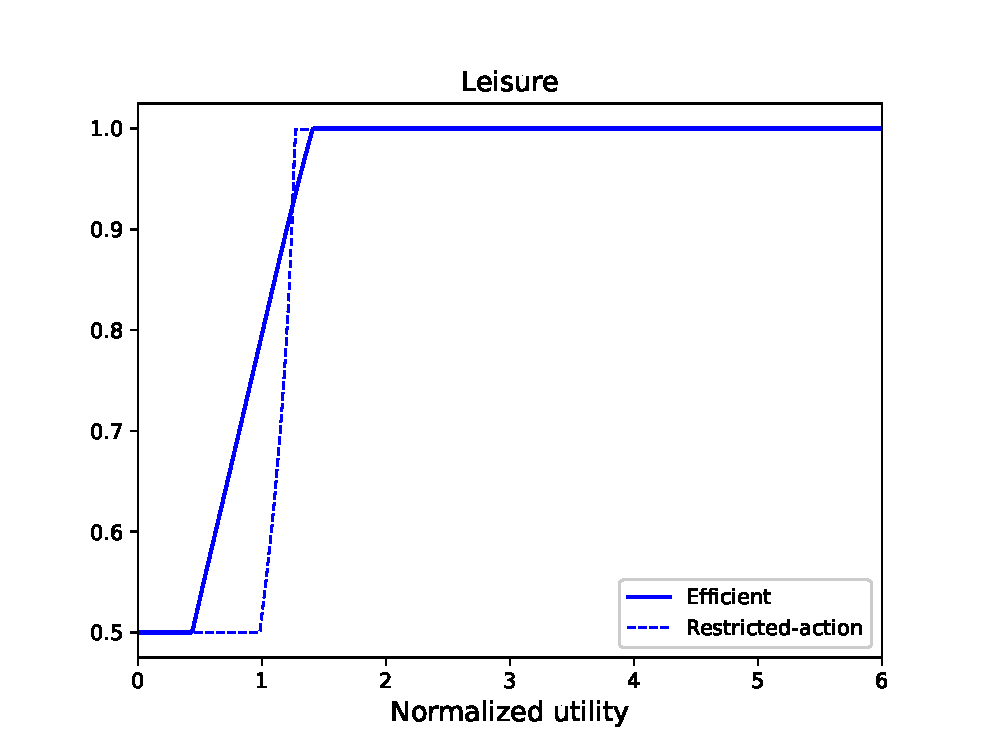
\includegraphics[width=0.49\linewidth]{leisure_ex}
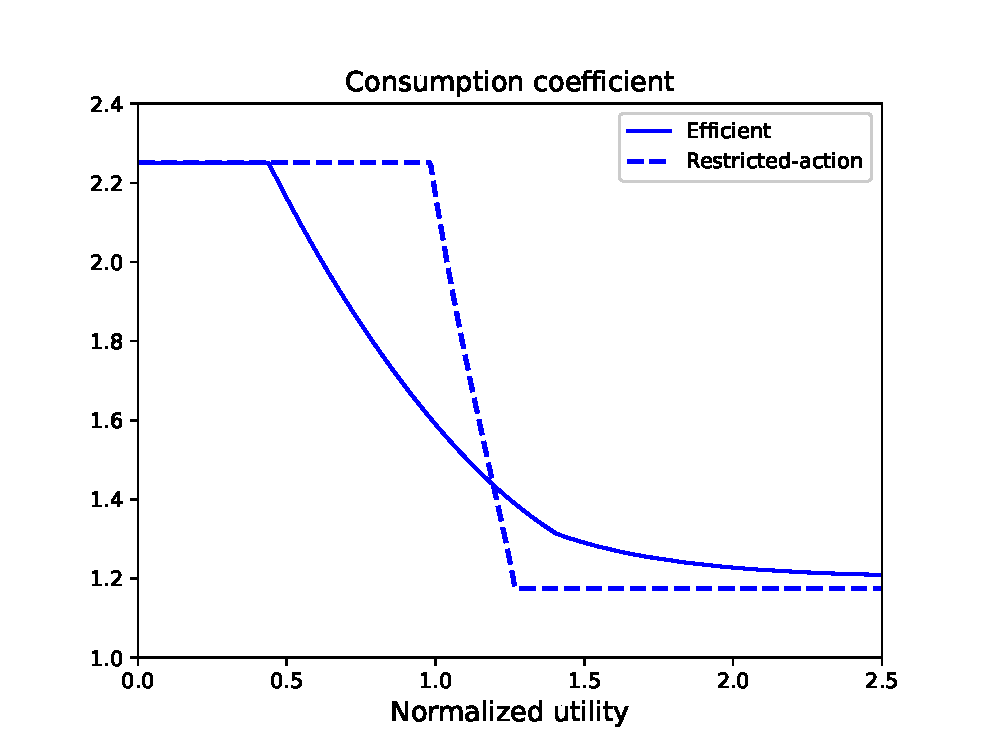
\includegraphics[width=0.49\linewidth]{consumption_ex}
\caption{Efficient and restricted-action leisure and consumption.}\label{fig:l_c}
\end{figure}

However, as emphasized above, the persistent effects of effort on output in this environment has important implications for the evolution of normalized utility, and lead it to differ qualitatively from the model of \cite{sannikov_continuous-time_2008}. Figure \ref{fig:law_u} plots the risk-adjusted growth in normalized utility and the volatility of normalized utility in both the efficient and optimal restricted-action cases. As noted subsequent to Lemma \ref{lawu}, the risk-adjusted growth in normalized utility is the difference between two terms, the first representing the risk-adjusted growth in the utility and the second the risk-adjusted growth in output. As expected, for low levels of output, the principal recommends high effort (low leisure), and the risk-adjusted growth in normalized utility is negative. Further, in Figure \ref{fig:law_u} the volatility of normalized utility is everywhere negative in both the efficient and the restricted-action allocations. When combined with the monotonicity of the leisure function, this implies that high realizations of productivity growth lead to lower normalized utility and therefore higher effort recommended by the principal. More succinctly, higher shocks lead to higher risk in future utility, and so as time goes on, the ``rich'' typically work harder and bear more risk than the ``poor'' in efficient allocations. 

\begin{figure}[!htb]
\centering
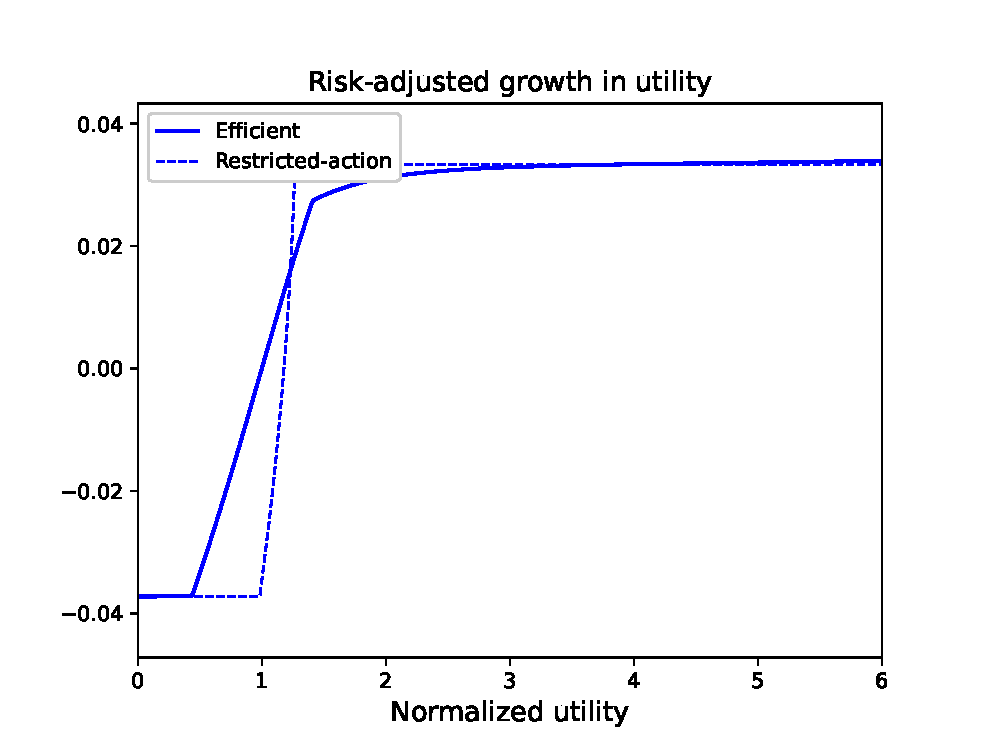
\includegraphics[width=0.49\linewidth]{risk_adj_ex}
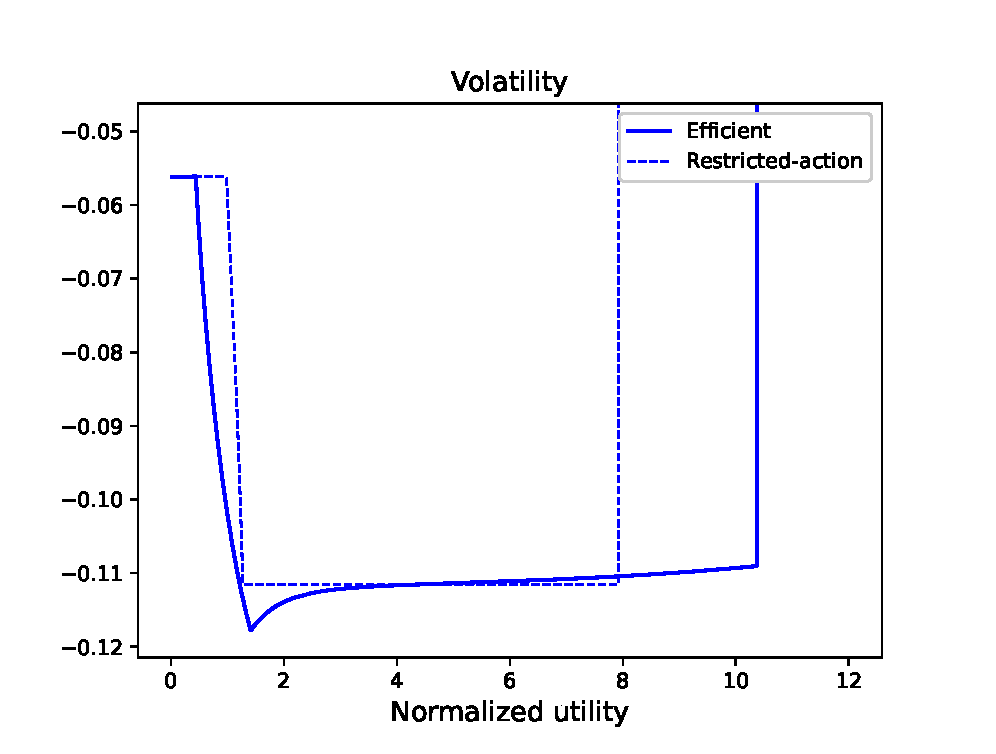
\includegraphics[width=0.49\linewidth]{sig_u_ex}
\caption{Efficient and restricted-action law of motion for utility.}\label{fig:law_u}
\end{figure} %, as suggested by Lemma \ref{lawu})

Figure \ref{fig:l_c_log} in Appendix \ref{sec:add_figures} computes analogues of Figure \ref{fig:l_c} and Figure \ref{fig:law_u} when utility is logarithmic, which corresponds to the limit $\gamma \rightarrow 1$. In this case the risk-adjusted growth remains negative for small normalized utility, and the volatility is again everywhere negative, albeit closer to zero than in the $\gamma=2$ case. I emphasize that the volatility of normalized utility is not guaranteed to be negative for all parameters.\footnote{Indeed, it is easy to see that condition \eqref{fallNS} in Lemma \ref{lawu} can fail for, e.g., logarithmic utility and high discounting (high $\rho$) or higher preferences for leisure (higher $\alpha$).} However, the point of these examples is simply that the novel addition of persistent effects of effort can, in principle, completely reverse the relationship between output shocks and future effort, relative to the standard model of \cite{sannikov_continuous-time_2008}. Further, in addition to being satisfied for the parameters given here, Lemma \ref{lawu} shows that this reversal holds for all sufficiently high levels of risk. 

In all of the above cases the efficient functions inherit the qualitative features of their restricted-action counterparts, but exhibit greater smoothness and vary less abruptly with normalized utility. Indeed, in numerical experimentations I have observed a kind of ``bang-bang'' solution for policy functions, with the lowest leisure level chosen at low levels of normalized utility, and the highest chosen at high levels.\footnote{This phenomenon appears to be more likely to occur when the degree of idiosyncratic risk is small.}

%and so the net effect on incentives to deviate is \textit{a priori} ambiguous.

Before turning to the setting with a continuum of agents, it is instructive to compare the above optimal contract with those in other environments with hidden actions, and with the dynamics of income that obtain in economies with exogenously incomplete markets. This will also serve as a prelude as to why thick right tails of consumption and firm size emerge in this environment. \cite{shourideh_optimal_2013} and \cite{phelan_optimality_2022} both consider economies with hidden consumption. To preserve incentives for investment, the risk borne by entrepreneurs must scale with the benefits of diverting capital to consumption, and so rich agents with low marginal utility of consumption control high amounts of capital. With homothetic preferences, these forces cancel and the elasticity of consumption with respect to output is common across agents, and generates Pareto distributions in consuption and firm size. However, these two papers cannot generate the need for an active stock market in which share prices depend endogenously on the expected effort exerted by the owner.

%, although they generate heterogeneous capital income and a thick tail of the wealth distribution

It is also worth contrasting the lessons drawn from the current environment with the allocation in \cite{jones_schumpeterian_2018}. In their model entrepreneurs are assumed to be unable to save, and so consumption, income, and firm profits coincide. This differs sharply from the current paper, in which risk-sharing is restricted only by the need to provide incentives for effort. In particular, productivity growth affects consumption growth only insofar as it affects the return on effort and thereby the tightness of the incentive constraints. Consequently, although the stationary distributions of both consumption and firm size in the ensuing perpetual youth environment are both approximately Pareto, the right tail for firm size is typically thicker than that for consumption. Proposition \ref{RESTdist} below formalizes this by showing that the distributions associated with the restricted-action allocations may be characterized in closed-form. While the tail of the firm size distribution depends only on the technology governing productivity growth and may be arbitrarily thick, the desire to smooth consumption over time places tight bounds on the tail of the ensuing distribution. Before proceeding to the general equilibrium context, I conclude this section by noting that if output is scaled by $\kappa \geq 0$, then the principal behaves as if confronted with an agent of productivity $\kappa \theta$. This has the following simple (but important) consequence.

\begin{lemma} \label{scalehomog}
For any parameter $\kappa > 0$, denote the normalized value function associated with this level of productivity by $v(u;\kappa)$. Then for all $\kappa, u \geq0$, we have $v(u; \kappa) = \kappa v(u/\kappa; 1)$.
\end{lemma}

\noindent Lemma \ref{scalehomog} will prove useful in the general equilibrium setting when the productivity of entrepreneurs depends on an endogenous shadow price of labor. In what follows I will write $v(\cdot) \equiv v(\cdot;1)$ for the normalized payoff function associated with unitary productivity.

\section{Efficient stationary allocations} \label{GenEq}

The preceding section analyzed the optimal contract between a single risk-averse agent and a risk-neutral principal. This section shows how the problem of a planner in an overlapping-generations economy may be decomposed into a series of one-on-one principal-agent problems identical in form to those considered above. General equilibrium forces affect both the level of utility that may be given to a generation and the productivity of entrepreneurs, because the latter depends on the number of agents working for their business. 



%\subsection{Environment}


Time is again continuous and extends indefinitely. At any instant there is a continuum of agents alive in the economy with subjective discount factor $\rho_S$ who die at rate $\rho_D$, so the preferences of agents continue to be of the form in \eqref{prefagent} and \eqref{flowutil2} with discount rate $\rho := \rho_S+\rho_D$. A flow of $\rho_D$ agents are born every unit of time so that the total population is fixed at unity. Every agent alive at the initial date is indexed by a scalar $v$ identified with promised utility. For each agent there is an associated process $(Z^v_t)_{t\geq0}$ distributed according to standard Brownian motion and referred to as the noise process for the agent. The noise processes for subsequent generations will be indexed by their date of birth. These processes are independent of one another and so by a law of large numbers the ex-post distribution of shocks across agents will coincide with the ex-ante distribution faced by each agent. 

Agents may be one of two types, entrepreneurs and workers, which are permanent and unobservable. A fraction $\eta_E \in [0,1]$ are entrepreneurs and the remaining $1-\eta_E$ are workers. Entrepreneurs are distinguished from workers by their ability to run businesses and have productivity that evolves as in Section \ref{PriAg}, $d\theta^v_t = \mu_{\theta}(l_t)\theta^v_tdt + \sigma_{\theta}(l_t)\theta^v_t dZ^v_t$ and satisfies $\theta_0 = 1$. In Section \ref{PriAg} the output of an entrepreneur coincided with his productivity. In contrast, in this section the output of an entrepreneur is a function of both their productivity and the effective labor assigned to him. If an entrepreneur of productivity $\theta$ is assigned $L$ units of effective labor, then for a fixed $Z>0$ and $\beta \in (0,1)$ flow output of their firm is $F(\theta,L) = Z\theta^{1-\beta}L^{\beta}$ per unit of time. To ensure that output is finite in the stationary distribution I will also suppose that $\rho_D > \mu_{\theta}(l)$ for all leisure levels. All workers inelastically supply $\overline{L}$ units of effective labor per unit of time, while entrepreneurs oversee production and provide no effective labor, and so I omit labor supply from the definition of an allocation. 


An allocation must specify the consumption, effort exerted, and labor assigned to every member of the initial generation as a function of initial promised utility, type, and history of output, together with analogous quantities for all subsequent generations as functions of birth date and type. In the following $L^{v,\theta,i}_t$ and $L^{T,i}_t$ refer to the effective labor assigned \textit{to} a given type (which vanishes if $i=W$), and for agents not alive at the initial date, the superscript refers to birth date and the subscript to calendar time.

\begin{defn} \label{defnALLOC}
Given a distribution $\Phi$ over utility, productivity, and types, an allocation consists of sequences $(c^{v,\theta,i}_t,l^{v,\theta,i}_t,L^{v,\theta,i}_t)_{t\geq 0}, \ (v,\theta,i) \in \textnormal{supp}(\Phi)$ for the initial generation and $(c^{T,i}_t, l^{T,i}_t,L^{T,i}_t)_{t\geq T \geq 0}, i = E,W$, for subsequent generations. An allocation satisfies promise-keeping if $U(c^{v,\theta,i},l^{v,\theta,i})= v$ for all $(v,\theta,i) \in \textnormal{supp}(\Phi)$.

\end{defn}
I will denote the set of all allocations by $\mathcal{A}$, and I will denote aggregate consumption, labor assignments, output, and (flow) utility by $C_t, L_t, Y_t$ and $U_t$, respectively.\footnote{Formal definitions are contained in Appendix \ref{planPREFapp}.} 

\begin{defn}
An allocation is resource feasible if it satisfies $C_t \leq Y_t$ and $L_t \leq \overline{L}$ for all $t\geq0$. The set of such allocations will be denoted $\mathcal{A}^{RF}$.
\end{defn}

Incentive-compatibility requirements are of two kinds: an entrepreneur must be induced to reveal her type at birth and then to follow the effort recommendations of the planner. Incentive compatibility must, in principle, account for the possibility of double deviations, in which an agent misreports her type and then deviates from the recommended action. However, such double deviations are irrelevant here, since an entrepreneur who claims to be a worker is subject to no further private information. 

\begin{defn}
The consumption and leisure allocations for a particular generation are incentive compatible if for all leisure strategies $l'$, $U_E(c^E,l) \geq \max\left\{ U_E(c^E,l'), U_W(c^W,1)\right\}$. The set of incentive-compatible allocations will be denoted $\mathcal{A}^{IC}$ and the set of allocations that are incentive compatible and resource feasible is denoted $\mathcal{A}^{IF} := \mathcal{A}^{RF} \bigcap \mathcal{A}^{IC}$.
\end{defn}

%Agents have preferences solely over their own consumption and effort and there is no altruism across generations. 

For simplicity I will suppose that the planner only cares about workers and places a weight of $\alpha(T) = e^{-\rho_S T}$ on an agent born at time $T$.\footnote{This is equivalent to weighing flow utility independently of an agent's birth date. To aid the reader, elaboration of the social welfare function is given in Appendix \ref{planPREFapp}.} I now relate the planner's problem to the principal-agent problems of Section \ref{PriAg}. 
\begin{defn}
Given an initial distribution $\Phi$ over promised utility and types, the planner's problem is defined to be $V(\Phi) = \max_{A \in \mathcal{A}^{IF}} U^P(A)$.
\end{defn} 
As in \cite{farhi_inequality_2007} I focus on solutions in which the distributions of productivity and utility are constant over time. To this end, I first consider the simpler problem of a planner who may trade goods and labor intertemporally at the subjective rate of time preference. If we solve this \textit{relaxed} problem and the implied distributions are constant over time, then we have solved the planner's problem beginning at that distribution. The relaxed problem has only two constraints and so the interdependence across agents is captured by two Lagrange multipliers, and so one need only maximize the components of the objective relevant to each generation in isolation. The only differences between this problem and the principal-agent problem analyzed in Section \ref{PriAg} are the requirement that the utility of an entrepreneur be sufficiently high to ensure truthful revelation, and the static task of assigning workers to entrepreneurs. At any moment the latter task depends solely on the shadow price of labor and productivity and solves $\max_{L \geq 0} \ Z\theta^{1-\beta} L^{\beta} - \lambda_LL$, the solution of which requires only elementary algebra and is summarized as follows. 

\iffalse
\begin{defn}
Given an initial distribution $\Phi$, the relaxed problem of the planner is
\begin{align*}
V^R(\Phi) = \max_{A \in \mathcal{A}^{IC}} \
\int_0^{\infty} e^{-\rho_S t} U_t & dt
\\ \int_0^{\infty} e^{-\rho_S t}(C_t - Y_t)dt & \leq 0
\\ \int_0^{\infty} e^{-\rho_S t}(L_t - \overline{L})dt & \leq 0.
\end{align*}
\end{defn}
\fi

\begin{lemma} \label{STATlemma}
Given the multiplier $\lambda_L$, labor assigned to an entrepreneur of productivity $\theta$ is $L(\theta) = [Z\beta/\lambda_L]^{\frac{1}{1-\beta}} \theta$. Flow output and output net of labor costs are $(1-\beta)^{-1}\overline{Z}(\lambda_L)  \theta$ and $\overline{Z}(\lambda_L) \theta$, respectively, where $\overline{Z}(\lambda_L) := (1-\beta)Z^{\frac{1}{1-\beta}}(\beta/\lambda_L)^{\frac{\beta}{1-\beta}}$.
\end{lemma}

\iffalse
\begin{align*}
Z\theta^{1-\beta}L(\theta)^{\beta} & = Z\theta   [Z\beta/\lambda_L]^{\frac{\beta}{1-\beta}}  = Z^{\frac{1}{1-\beta}}(\beta/\lambda_L)^{\frac{\beta}{1-\beta}} \theta
\\ Z\theta^{1-\beta}L(\theta)^{\beta} - \lambda_LL(\theta) & = Z^{\frac{1}{1-\beta}}((\beta/\lambda_L)^{\frac{\beta}{1-\beta}} - \lambda_L[\beta/\lambda_L]^{\frac{1}{1-\beta}})\theta
\\ & = Z^{\frac{1}{1-\beta}}(\beta^{\frac{\beta}{1-\beta}}\lambda_L^{-\frac{\beta}{1-\beta}} - \lambda_L^{-\frac{\beta}{1-\beta}}\beta^{\frac{1}{1-\beta}} )\theta
\\ & = Z^{\frac{1}{1-\beta}}\lambda_L^{-\frac{\beta}{1-\beta}}(\beta^{\frac{\beta}{1-\beta}} - \beta^{\frac{\beta}{1-\beta}+1} )\theta
\end{align*}
Write: $u = [(1-\gamma)U]^{\frac{1}{1-\overline{\gamma}}}$ and so $u^{1-\overline{\gamma}}/(1-\gamma) = U$, or $U = \frac{u^{1-\overline{\gamma}}}{1-\gamma} = \frac{(\overline{Z}\lambda_L^{-\frac{\beta}{1-\beta}})^{1-\overline{\gamma}}}{1-\gamma}$. $y := \overline{Z}^{-1}\lambda_L^{\frac{\beta}{1-\beta}}u$. 
This amounts to solving the generational planner's problem and then varying the shadow prices of goods and labor until the resource constraints hold in the associated stationary distribution. 
The stationary form of the goods and labor resource constraints are then
\begin{equation}
\begin{aligned}
0 & = \int_{\Omega'}\mathbb{E}[c^{v,\theta,i} - F(\theta^{v,\theta,i},L^{v,\theta,i})]\Phi_{\lambda}(d\omega')
\\ 0 & = \overline{L} - \int_{\Omega'}\mathbb{E}[L^{v,\theta,i}]\Phi_{\lambda}(d\omega').
\label{steadyR}
\end{aligned}
\end{equation}
The first equation in \eqref{steadyR} imposes the requirement that aggregate consumption equal aggregate output, while the second imposes the requirement that the total stock of effective labor coincide with the aggregate amount assigned to entrepreneurs. If $\lambda$ satisfies \eqref{steadyR}

For any multiplier there will be a stationary density of normalized utility that depends only on the policy functions associated with unitary productivity. 
\fi

Given a pair of multipliers $\lambda := (\lambda_R, \lambda_L)$, denote the associated stationary distribution over $\Omega' := \mathbb{R} \times \Theta \times \{E,W\}$ by $\Phi_{\lambda}$. If this distribution satisfies the resource constraints then the solution to the relaxed planner's problem with initial distribution $\Phi_{\lambda}$ amounts to adhering to the solutions to the generational planner's problem. I now combine the above with the optimal contract characterized earlier in partial equilibrium to infer properties of the long run distributions of consumption and productivity. Just as the homotheticity of preferences allowed for a simplification of the principal's problem, so too do the linear policy functions imply that when calculating aggregate quantities we need only restrict attention to a one-dimensional distribution.

\begin{defn}\label{summary_m}
Given a distribution $\Phi$ over the productivity and normalized utility, the summary measure is defined by $m(B) = \int_{B}\int_{0}^{\infty} \theta\Phi(\theta,u) d\theta du$ for any $B \subseteq [0, \infty)$.
\end{defn} 

The homogeneity of the policy functions ensures that aggregate quantities may be expressed in terms of this summary measure. For instance, the average productivity and consumptin of entrepreneurs is $\int_{0}^{\infty}m(u)1_{l(u)<1} du$ and $\int_{0}^{\infty}c(u)m(u) du$, respectively. One implication of Lemma \ref{STATlemma} is that changes in the shadow price of labor cause changes in the productivity of every entrepreneur, with payoffs remaining proportional to $\theta$. When combined with Lemma \ref{scalehomog}, this implies that changes in resource constraints only affect normalized utility, with the subsequent policy functions identical to those found in the setting of Section \ref{PriAg}. For any initial $\overline{u}$ denote the implied stationary density by $m_{\overline{u}}$, and note that the average productivity and consumption of entrepreneurs per unit of aggregate productivity in the stationary distribution may be written
\begin{equation}
\begin{aligned}
M(\overline{u}) & := \int_{0}^{\infty}m_{\overline{u}}(u)1_{l(u)<1}du \ \ \ \ \ & \ \ \ \ \
C(\overline{u}) & := \int_{0}^{\infty}c(u)m_{\overline{u}}(u)du.
\label{Output}
\end{aligned}
\end{equation} 
Since workers have constant consumption throughout their lifetime, the associated aggregate consumption of workers is simply $(1-\eta_E)\overline{Z}(\lambda_L)\overline{u}$. It remains to determine aggregate labor demand and consumption as functions of the multipliers and find conditions under which resources balance. Given an initial $\overline{u}$ the labor resource constraint reduces to
\begin{equation}
\begin{aligned}
\overline{L} & = (\textnormal{ave.} \ \theta) \times \textnormal{(no. entrepreneurs)} \times \textnormal{(labor per $\theta$)}
\\ & = M(\overline{u}) \times \eta_E \times {\left(Z\beta/\lambda_L\right)}^{\frac{1}{1-\beta}}.
\end{aligned}
\label{LRcons7}
\end{equation}
Characterizing efficient allocations then reduces to solving a single nonlinear equation. 
\begin{prop}\label{STAT1}
The stationary level of normalized utility is the solution to 
\begin{equation}
\frac{\eta_E}{1-\beta}M(u) = (\eta_EC(u)/u + 1 - \eta_E)u
\label{STATy}
\end{equation}
with the associated level of utility in consumption units $(1-\beta)Z(\eta_EM(u))^{-\beta}\overline{L}^{\beta}u$. 
\end{prop}
\begin{proof}
From Lemma \ref{STATlemma} the output of each firm is $(1-\beta)^{-1}\overline{Z}(\lambda_L)\theta$. Using \eqref{LRcons7} and integrating over all firms, aggregate output and consumption in the stationary distribution are $\eta_E(1-\beta)^{-1}\overline{Z}(\lambda_L)M(u)$ and $\overline{Z}(\lambda_L){\left(\eta_EC(u) + (1-\eta_E)u\right)}$, respectively. Dividing output and consumption by $\overline{Z}(\lambda_L)$ gives \eqref{STATy} and rearranging \eqref{LRcons7} gives utility. 
\end{proof}
Proposition \ref{STAT1} shows that to determine the constrained-efficient stationary distribution, the value function need only be calculated once even though there is a continuum of agents and two resource constraints. This allows for simple comparative statics. 
\begin{corl} \label{compstat3}
The stationary level of normalized utility is increasing in $\eta_E$ and $\beta$ and independent of $Z$.
\end{corl}
\begin{proof}
Define $H(y) :=  M(y)(1-\beta)^{-1} - C(y) - y(1-\eta_E)/\eta_E$ and note that the stationary normalized utility is a root of $H$. All the claims follow from Topkis' theorem and the fact that $H$ is increasing in $\eta_E$ and $\beta$ and independent of $Z$. 
\end{proof}
The third claim in Corollary \ref{compstat3} may be viewed as a neutrality result, as it shows that changes in total factor productivity have no effect on the stationary value of normalized utility. Such changes therefore have no effect on inequality in the associated stationary distributions of consumption and firm size, as these are simply scaled for all agents after every history by the same amount. 

Proposition \ref{propREST} shows that the restricted value and policy functions associated with the highest action are good approximations to the true value and policy functions for low levels of normalized promised utility. Since agents with low normalized utility have high productivity and so typically high consumption, one expects the right tail of the consumption distribution to look similar to that associated with the restricted-action allocation for the highest effort level, and this is what is observed in all simulations. To extend the discussion following Lemma \ref{lawu} and highlight how the efficient allocations of this paper differ from the exogenously incomplete markets model of \cite{jones_schumpeterian_2018}, I now consider the stationary distributions associated with the restricted-action policy functions. This will also serve as a prelude to the results of Section \ref{Imp}, where it is shown that these distributions correspond to those that are implemented with linear taxes in a signaling equilibrium. The formulation of the stationary resource constraints is simpler and more transparent in this case. Recall from the discussion following Proposition \ref{propREST} that $v^*_{\textnormal{r}}$ and $l_{\textnormal{r}}^*$ denote the value and policy functions of a principal who must recommend the same leisure level for the entirety of an agent's life. In this case consumption growth is characterized by constant mean and volatility, and so for any leisure level $l$ the stationary resource constraint becomes
$$
Z{\left(\frac{\rho_D\eta_E}{\rho_D - \mu_{\theta}(l)} \right)}^{1-\beta}\overline{L}^{\beta} = {\left(\frac{\rho_D \eta_E\overline{c}_{\textnormal{r}}(l)}{\rho_D - \mu_c(l)} + 1 - \eta_E\right)}[(1-\gamma)U]^{\frac{1}{1-\overline{\gamma}}}
$$
where $U$ denotes lifetime utility. Imposing the labor resource constraint once more and simplifying gives the following analogue of Proposition \ref{STAT1} and Corollary \ref{compstat3}.

\begin{prop}\label{RESTchar}
The optimal restricted-action leisure level is $l_{\textnormal{r}}^*(u_{\textnormal{r}})$, where $u_{\textnormal{r}}$ solves 
$$
\frac{\rho_D \eta_E (1-\beta)^{-1}}{\rho_D - \mu_{\theta}(l_{\textnormal{r}}^*(u_{\textnormal{r}}))} = {\left(\frac{\rho_D \eta_E\overline{c}_{\textnormal{r}}(l_{\textnormal{r}}^*(u_{\textnormal{r}}))}{\rho_D - \mu_c(l_{\textnormal{r}}^*(u_{\textnormal{r}}))} + 1 - \eta_E\right)}u_{\textnormal{r}}.
$$
The associated utility is $\overline{Z}u_{\textnormal{r}}$ where $\overline{Z} = (1-\beta)Z{\left(\rho_D - \mu_{\theta}(l_{\textnormal{r}}^*(u_{\textnormal{r}}))\right)}^{\beta}(\overline{L}/[\rho_D\eta_E])^{\beta}$ and $l_{\textnormal{r}}^*(u_{\textnormal{r}})$ is increasing in both $\eta_E$ and $\beta$.
\end{prop} %\overline{Z} = (1-\beta)Z{\left(\frac{\rho_D\eta_E}{\rho_D - \mu_{\theta}(l_{\textnormal{r}}^*(u_{\textnormal{r}}))}\right)}^{-\beta}\overline{L}^{\beta}

It is well-known that the stationary distribution of a geometric Brownian motion that is killed at a constant rate and reinjected at some point $\overline{X}$ has a stationary distribution of the \textit{double-Pareto} form $f(x) = A x^{\alpha^+_X-1}1_{x \leq \overline{X}} + B x^{\alpha^-_X-1}1_{x > \overline{X}}$ for some $A,B > 0$ and tail parameters $\alpha^{\pm}_X$. The expressions in Proposition \ref{propREST} then lead to the following characterization. A proof is contained in Appendix \ref{restDISTsect}.

\begin{prop}\label{RESTdist}
For each $l \in [\underline{l},1]$ the stationary distributions of consumption and firm size associated with the restricted-action allocation with leisure $l$ are both double-Pareto. The tail parameters for consumption are 
$$
\alpha^{\pm}_c (l) = -\frac{\overline{\gamma}}{2}  \pm  \frac{\overline{\gamma}}{2}\sqrt{1 + \frac{4\rho_D(1 - 1/\overline{\gamma}) (2-1/\overline{\gamma})}{\rho(1-x(l))}} 
$$ 
and the tail parameters for firm size (in output or employment) are 
$$
\alpha^{\pm}_\theta (l) = \mu_{\theta}(l)/\sigma^2 - 1/2 \pm \sqrt{(\mu_{\theta}(l)/\sigma^2 - 1/2)^2 + 2\rho_D/\sigma^2}.
$$
\end{prop}  %\footnote{And also note that $\alpha_\pm (l) \rightarrow -\overline{\gamma}$ as the death rate vanishes.} 
Proposition \ref{RESTdist} illustrates that the forces governing the distributions of firm size and consumption are very different from one another. For a given level of effort, the tail of the firm size distribution is mechanically determined by technological parameters.\footnote{A finite mean is assured if $\alpha_{\theta}^-(l) < -1$, which is implied by the assumption $\rho_D > \mu_{\theta}(l)$.} In contrast, consumption growth depends on the technological parameters only insofar as the latter affect the tightness of the incentive constraints. Indeed, Proposition \ref{RESTdist} shows that we have the uniform bound $\alpha_\pm (l) \leq -\overline{\gamma}$ for the tail parameter for consumption, independent of the nature of the agency problem. This places strong restrictions on the degree of inequality that can arise in efficient allocations, and shows that the implied distributions contrast sharply with models with exogenously incomplete markets, such as \cite{jones_schumpeterian_2018}, in which the tails of firm size and consumption are forced to coincide by assumption. 

I now illustrate these points by plotting the upper tail parameters for consumption and firm size with $\rho_D = 0.04$ and the same parameters adopted in Figure \ref{fig:l_c}. Following \cite{jones_schumpeterian_2018}, one need not view $\rho_D$ literally as the probability of death, but rather the rate with which one ceases to be an entrepreneur, so that the above choice amounts to assuming that agents run their business for an average of 25 years and discount at rate $\rho = \rhoval$. On the left-hand side of Figure \ref{fig:tails} all parameters except for leisure coincide with Figure \ref{fig:l_c}, while on the right-hand side leisure is set at the lowest value and the volatility varies. As suggested by the above discussion, for all parameters plotted the tail of firm size is far thicker than that of consumption. Figure \ref{fig:tails_log} in Appendix \ref{sec:add_figures} repeats this exercise with $\gamma=1$ (logarithmic utility), which leaves the tail parameters for firm size unchanged but increases the thickness of the tails for consumption.

%\footnote{Figure \ref{fig:tails_log} differs from the analogous figure in the 2021 version due to a coding error which lead consumption to be too fat (the  ordering between $\overline{\gamma}=1$ and $\overline{\gamma}=2$ are the same).}  

\begin{figure}[!htb]
\centering
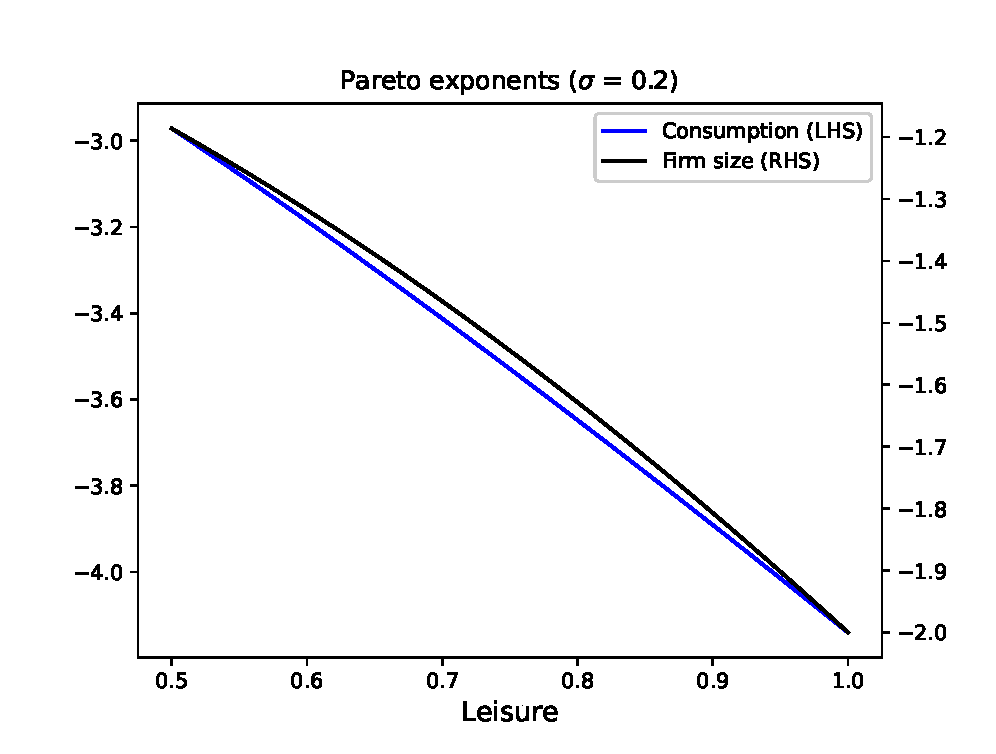
\includegraphics[width=0.49\linewidth]{tails}
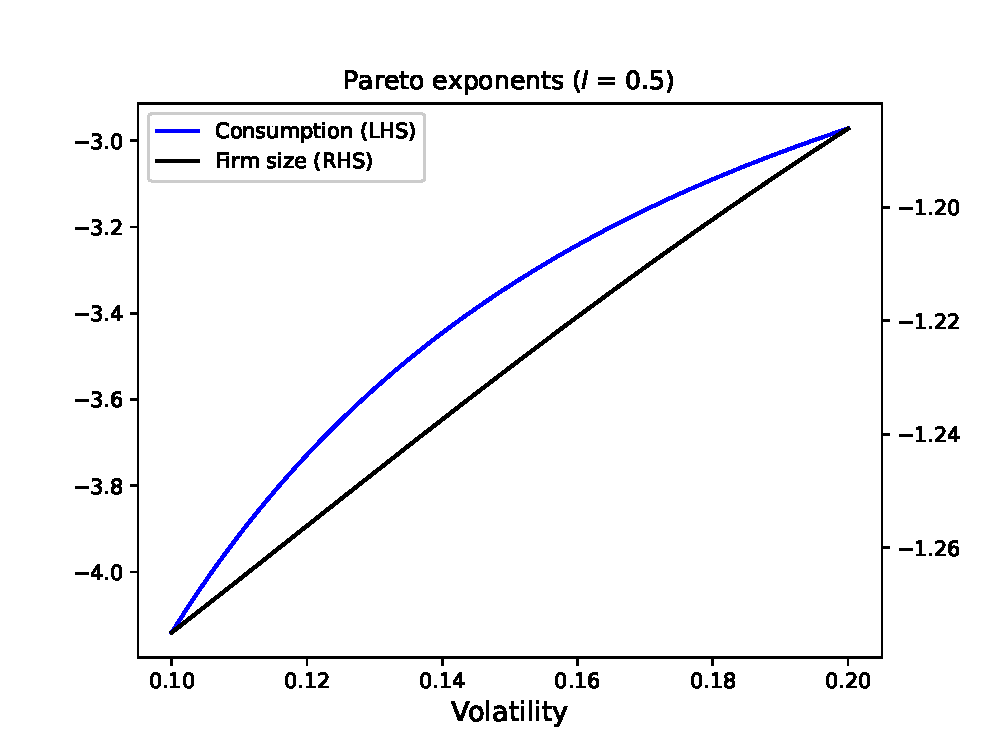
\includegraphics[width=0.49\linewidth]{tails_sig}
\caption{Tail parameters for firm size and consumption with $\gamma=2$.}\label{fig:tails}
\end{figure}



%For simplicity I now assume that $\rho = \overline{\mu}_0$ and $\overline{\mu}_1 = 0$.\footnote{These assumptions do not drive the qualitative results that follow but simplify the associated algebra.}

\section{Optimal linear taxes} \label{Imp}

The foregoing analysis has focused on the forces that shape the long run efficient levels of inequality in an economy with repeated moral hazard, with all quantities implicitly specified by a social planner administering the direct mechanism. In this final section I discuss some implications for taxes. Prescriptions for taxes depend crucially on the contracts agents are capable of writing and enforcing. Indeed, at one extreme, by extending the results of \cite{atkeson_efficient_1992}, when agents may write contracts of arbitrary complexity with intermediaries, the optimal policy consists only of lump-sum transfers between agents. However, the assumption of such a sector of intermediaries is quite strong, and so in this final section I fix a market structure and characterize the allocations attainable with constant linear taxes. I will draw on the characterization of the optimal constant-leisure allocations in Section \ref{GenEq} in order to understand how the decision to retain equity depends on taxation policy, and to highlight the distinct effects of taxes on profits, savings and wealth. 


All agents may trade a risk-free government bond, and at the initial date, entrepreneurs decide on the fraction of their wealth that they will retain in their business in perpetuity, with the remaining shares sold to risk-neutral investors. The government levies constant linear taxes on firm profits and the owner's income and wealth, together with lump-sum transfers to workers. The choice of share retention of the entrepreneur is observable to all investors, who subsequently use this to form expectations of the entrepreneur's (unobservable) effort. The equilibrium notion will impose the requirement that these expectations be consistent with the choices of entrepreneurs, so that investors make zero expected profits.\footnote{This equilibrium notion differs from that adopted in earlier drafts, in which agents behaved competitively. Appendix \ref{eqcompare} discusses these two solution concepts and shows that although they lead to different taxes, they raise the same amount of revenue whenever both allocations are well-defined.}


This market structure allows one to distinguish between firm profits, capital gains, and interest income, instead of absorbing them all into the category of ``capital income'', as would be the case if agents could only save in a risk-free bond. The primary result of this section is that taxes on profits, interest income, and wealth play conceptually distinct and complementary roles, and that the tax on capital gains is redundant. The tax on profits achieves redistributive aims, the tax on interest income affects the incentives of owners to retain equity in their firm and exert effort, and the tax on wealth affects the degree of consumption smoothing over time. The allocations that arise with linear taxes coincide exactly with the restricted-action allocations characterized in Proposition \ref{RESTdist}, and the optimal taxes are simply chosen to ensure that the entrepreneurs exert the level of leisure given in Proposition \ref{RESTchar}. Consequently, even entrepreneurs with arbitrarily high wealth continue to exert effort, and the distributions of both firm size and wealth exhibit fat (Pareto) tails with indices that will, in general, differ from one another. 


I first describe the problem of an entrepreneur who has already committed to retaining a fraction of wealth in their firm, before turning to a discussion of this initial decision and of the appropriate equilibrium notion. The sole state variable for the entrepreneur will be financial wealth $a_t$, which is the sum of savings $b_t$ and the value of firm equity $p_tx_t$, where $x_t$ is the fraction of the firm owned by the agent and $p_t$ is the (endogenous) share price, 
\begin{equation}
a_t := b_t + p_tx_t. 
\label{totalass}
\end{equation} 
Consistent with the assumptions of Section \ref{GenEq}, I assume that entrepreneurs earn income only from business profits, interest and capital gains, and do not simultaneously receive a wage.\footnote{This assumption does not drive the results that follow. The presence of wage income would complicate the choice of share retention but not the savings or effort choices, as consumption would simply be a constant fraction of total wealth, inclusive of the discounted value of labor income.} All agents may save in a risk-free government bond with before-tax return $r_t$. I also assume the existence of a competitive sector of insurance companies who trade actuarially fair annuity contracts with agents, promising a return $\rho_D$ on the savings of agents in exchange for taking possession of these savings at death. The outside investors are risk-neutral, and so the price per share will equal the expected discounted value of firm profits, given the investors' expectations regarding the effort of the entrepreneur. The equilibrium notion outlined below will impose the requirement that these beliefs are correct, so that the outside investors break even in expectation. When investors believe that the effort exerted follows the process $\hat{l}$ and dividends are taxed according to the process $\tau_d$, they value the firm at
\begin{align*}
p_t = \mathbb{E}^{\hat{l}}{\left[\int_t^{\infty}e^{-(r+\rho_D)(s-t)} (1-\tau_{ds})\overline{Z}(w_s) \theta_sds\right]},
\end{align*}
where I remind the reader that $\overline{Z}$ is defined in Lemma \ref{STATlemma} as output per unit of productivity net of labor costs (i.e. profits per $\theta_s$), viewed as a function of the wage. If expectations and prices are constant (as they will be in the stationary equilibria we consider below), then the price of the firm is simply given by the Gordon growth formula
\begin{equation}
p_t = \frac{(1-\tau_d)\overline{Z}(w)\theta_t}{r + \rho_D - \mu_{\theta}(\hat{l})}
\label{priceRE}
\end{equation}
for all $t\geq0$ almost surely. Note that because the share market is competitive, investors will make zero expected profits from every trade with entrepreneurs. The following allocation and taxes are therefore unchanged if share purchases are executed by the government rather than private agents. In this latter case, government policy partially alleviates frictions in capital markets just as the taxation of labor income partially substitutes for the absence of insurance in the labor market.


When leisure expectations $\hat{l}$ and taxes $(\tau_d,\tau_s,\tau_{cg},\tau_a)$ on dividends, interest (the return on savings), capital gains, and wealth are constant over time, the entrepreneur's wealth evolves according to
\begin{equation}
da_t = [(1-\tau_s)(r + \rho_D) - \tau_a - \overline{c}_t]a_tdt + \overline{\iota}_t a_tdR_t(l_t;\hat{l})
\label{linearP3}
\end{equation}
where $\overline{c}_t$ and $\overline{\iota}_t$ denote the fraction of wealth consumed and invested, respectively, and 
\begin{equation}
dR_t(l_t;\hat{l}) = (\tau_s (r + \rho_D) + (1- \tau_{cg})\mu_{\theta}(l_t) - \mu_{\theta}(\hat{l}))dt + \sigma(1-\tau_{cg}) dZ_t.
\label{return}
\end{equation}
To understand the above law of motion of wealth, note that the expected after-tax excess return on investing in the agent's business is the sum of after-tax dividends and capital gains minus the after-tax return on the risk-free bond, or 
$$
(1 - \tau_d)\overline{Z}\theta_t/p_t + (1 - \tau_{cg})\mu_{\theta}(l_t) - (1 - \tau_s)(r + \rho_D).
$$
When combined with the price-earnings ratio given in \eqref{priceRE}, this gives the expression for the infinitesimal return \eqref{return}.\footnote{To aid the reader in the interpretation of the market structure and timing, a discrete-time formulation of the law of motion is contained in Appendix \ref{discCE}.} Notice that one implication of the expression \eqref{return} is that although the expected return is increasing in the effort of the entrepreneur, it is decreasing in the effort expected by investors, because high effort expectations imply a high price-earnings ratio, and hence low dividends per unit of equity retained. 


Before turning to a formal definition of the entrepreneur's problem, there are several aspects of the law of motion of wealth in \eqref{linearP3} that are worth discussing. First, it is important to note the distinction between $\hat{l}$ and $l$: the former is determined by the level of effort expected by investors while the latter is determined by the effort exerted by the agent. The two must coincide in equilibrium but only the latter is directly chosen by the entrepreneur, with the former jointly determined by the initial choice of share retention and the taxation policy of the government. Second, firm size does not appear in the law of motion of wealth, because with constant expectations, the price-dividend ratio is constant and hence so too is the expected return on retained equity. Third, the tax on firm profits and the wage also do not appear in the law of motion of wealth, because these only affect the value of the firm and hence the initial wealth of the agent, and not its evolution over time. 


The fact that the restricted-action allocations are characterized by three constants implies that we should expect one degree of freedom in our choice of the four taxes. For simplicity I therefore assume that capital gains are not taxed, as this simplifies the expressions that follow (but is not crucial for any results). I will also suppose that the government borrows and lends to the agents at rate $r = \rho_S$ and runs a primary surplus or deficit to balance its budget. In this case, the return on retained equity simplifies to
\begin{equation}
dR_t(l_t;\hat{l}) = (\tau_s \rho + \mu_{\theta}(l_t) - \mu_{\theta}(\hat{l}))dt + \sigma dZ_t
\label{return_simp}
\end{equation}
and so whenever the expected and actual leisure levels coincide, the expected excess return on equity is simply $\tau_s \rho$. Note that this excess return is increasing in the tax on interest because the latter reduces the outside option available to the entrepreneur, the risk-free bond, but does not affect the earnings-price ratio, which by \eqref{priceRE} is always 
$$ %p = \frac{(1-\tau_d)\overline{Z}(w)\theta_t}{r + \rho_D - \mu_{\theta}(\hat{l})}
(1-\tau_d)\overline{Z}\theta_t/p_t = r + \rho_D - \mu_{\theta}(\hat{l}) = \rho - \mu_{\theta}(\hat{l})
$$
regardless of taxes. The fact that the tax on interest appears in the excess return on equity but the tax on wealth does not hints at why they play conceptually distinct roles in the below implementation. The tax on interest alters the relative returns on the two assets, while the tax on wealth simply affects the growth rate of consumption. 


I will now outline the entrepreneurs' problem and the equilibrium notion adopted in this setting. For clarity, I will split the individual problem in to two parts, first characterizing optimal consumption and effort consistent with a given level of share retention (and hence expectations of investors), before turning to the initial choice of share retention and the definition of equilibrium.\footnote{In the following I substitute $r = \rho_S$, so the pre-tax return on the bond is $\rho = \rho_S + \rho_D$.}

\begin{defn}  \label{conPROBlin2}
Given linear taxes $\tau = (\tau_s,\tau_a)$ and expectations governed by $\hat{l}$, the problem of an entrepreneur with wealth $a$ who has pledged to retain $\overline{\iota}$ of her wealth in the firm is
\begin{align*}
V(a; \overline{\iota}, \hat{l}) = \max_{\overline{c},l} & \ \mathbb{E}^l{\left[\int_{0}^{\infty}\rho e^{-\rho t}u(\overline{c}_ta_t,l_t)dt\right]}
\\ da_t & = [(1-\tau_s)\rho - \tau_a - \overline{c}_t]a_tdt + \overline{\iota}_t a_tdR_t(l_t;\hat{l})
\\ a_0 & = a
\end{align*}
where $dR_t$ is given by equation \eqref{return_simp}. 
\end{defn}

Using a homogeneity argument almost identical to that given in Lemma \ref{homogprod}, one may show that the optimal consumption is a constant fraction of wealth and that the optimal effort is constant. I therefore denote by $\overline{c}^*(\overline{\iota}, \hat{l})$ and $l^*(\overline{\iota}, \hat{l})$ the optimal choices of consumption and leisure for the problem in Definition \ref{conPROBlin2} given the retained wealth share $\overline{\iota}$ and expectations $\hat{l}$. Lemma \ref{FIXiota} below then shows that there is a unique solution $\hat{l}(\overline{\iota})$ to the equation $\hat{l} = l^*(\overline{\iota}, \hat{l})$, which is the leisure consistent with rational expectations and the incentives faced by the entrepreneur. The problem of the entrepreneur is therefore the following. 

\begin{defn} \label{conPROBlin3}
Given a wage $w$ and constant linear taxes $\tau = (\tau_d,\tau_s,\tau_a)$, the problem of an entrepreneur choosing the fraction of their initial wealth to retain is given by $\max_{\overline{\iota} \geq 0} V(\overline{a}_0(\overline{\iota}); \overline{\iota}, \hat{l}(\overline{\iota}))$, where 
$V$ is given in Definition \ref{conPROBlin2} and 
\begin{equation}
\overline{a}_0(\overline{\iota}) = \frac{(1-\tau_d)\overline{Z}(w)\theta_0}{\rho - \mu_{\theta}(\hat{l}(\overline{\iota}))}
\label{initiala}
\end{equation}
denotes the initial wealth of the owner as a function of $\overline{\iota}$.
\end{defn} %(and wealth of the entrepreneur) 

The form of the problem in Definition \ref{conPROBlin3} illustrates that the entrepreneur faces a simple tradeoff when considering the fraction of their wealth to retain in the firm at the initial date. On the one hand, retaining shares exposes them to idiosyncratic risk in wealth and hence consumption, which reduces their welfare. However, retaining shares also increases their subsequent incentives to exert effort, and so increases their initial wealth, because it increases the price outside investors are willing to pay per share at the initial date. Further, this tradeoff is endogenous to tax policy, because the excess return on equity depends on the tax on savings, and all investors rationally recognize this dependence. 


Given the above formulation of the market structure and expectation formations, the equilibrium notion I adopt is of a standard type: individuals optimize, markets clear, and expectations are consistent with individual incentives. 

\begin{defn}[Signaling equilibrium] \label{SIGE}
Given constant linear taxes $\tau$, a stationary signaling equilibrium consists of wages $w$, expectations $\hat{l}$, and policy functions $(\overline{c},l) = (\overline{c}_t,l_t,\overline{\iota})_{t\geq0}$ and $\overline{\iota}$ for consumption, leisure, and share retention, such that:
\begin{itemize}
\item The policy functions $(\overline{c},l,\overline{\iota})$ solve the consumer problem given in Definition \ref{conPROBlin2} and Definition \ref{conPROBlin3}, given expectations $\hat{l}$.  
\item The outside investors make zero expected profits, or $l_t = \hat{l}$ for all $t\geq0$ almost surely. 
\item The markets for goods and labor clear every instant. 
\item The government budget constraint is satisfied. 
\end{itemize}
\end{defn} 

Prior to characterizing signaling equilibria, I wish to emphasize once more why the characterization of restricted-action allocations in Section \ref{PriAg} is useful for determining the optimal linear taxes. Indeed, the mechanism design approach adopted earlier may be appear to be superfluous given that in this section we restrict attention to linear taxes and make no mention of incentive compatibility. However, the key insight here is that for any level of share retention, the solution to the problem in Definition \ref{conPROBlin2} with constant linear taxes implies constant effort by the entrepreneur. Given the planner's objective, these allocations are therefore weakly dominated by the restricted-action allocations, as the latter are, by definition, the optimal incentive compatible allocations with constant effort. Consequently, if we can implement the optimal restricted-action allocation as a signaling equilibrium, then we have found the optimal linear taxes, because the fact that entrepreneurs freely choose their consumption and (unobservable) leisure implies that the equilibrium allocation is incentive compatible. Further, Lemma \ref{lawu} shows that the restricted-action allocations are completely characterized by the initial consumption level and the constant mean and volatility of consumption growth. It will therefore suffice to find linear taxes such that these quantities in the signaling equilibrium coincide with their counterparts in the optimal restricted-action allocations, because then the allocations will coincide almost surely at every date. The following algebra simply shows how one may choose taxes to ensures that the mean consumption growth coincide across equiibrium and efficient allocations. 


I first characterize the expectations for effort consistent with a given choice of $\overline{\iota}$ and individual optimality, before turning to the initial choice of share retention. 

\begin{lemma} \label{FIXiotal}
Given a retained wealth share $\overline{\iota}$ and expectations $\hat{l}$, the optimal consumption and leisure choices are given by
%\begin{equation}
%\begin{aligned}
$$
\overline{c}(\overline{\iota}, \hat{l}) = \frac{\rho}{\gamma} + \frac{1}{\gamma}{\left([\overline{\mu}_0\hat{l} + \tau_s\rho]\overline{\iota} - \overline{\gamma}\sigma^2\overline{\iota}^2/2 - \tau_a + (1-\tau_s)\rho\right)}(\overline{\gamma} - 1) 
$$
%\end{aligned}
%\label{cbar}
%\end{equation}
and $l^*(\overline{\iota}, \hat{l})\overline{\mu}_0\overline{\iota}(1-\alpha) = \alpha \overline{c}(\overline{\iota}, \hat{l})$
provided that $l^*(\overline{\iota}, \hat{l}) \in [\underline{l}, 1]$. 
\end{lemma}


\begin{proof}
Given $(\overline{\iota}, \hat{l})$, I guess-and-verify that the value function of the agent is of the form $V(a) = \overline{V}a^{1-\overline{\gamma}}/(1-\gamma)$ for some $\overline{V}$. Substituting this form into the Hamilton-Jacobi-Bellman equation associated with the problem in Definition \ref{conPROBlin2} gives
\begin{equation}
\begin{aligned}
\frac{\rho \overline{V}}{1-\gamma} & = \max_{\substack{\overline{c} \geq 0 \\ l \in [\underline{l},1]}} \frac{\rho(\overline{c}^{1-\alpha}l^{\alpha})^{1-\gamma}}{1-\gamma} + [ - \tau_a - \overline{c} + (1-\tau_s)\rho](1-\alpha)\overline{V}
\\ & + {\left({\left[\mu_{\theta}(l) - \mu_{\theta}(\hat{l}) + \tau_s\rho\right]}\overline{\iota} - \overline{\gamma}\sigma^2\overline{\iota}^2/2\right)}(1-\alpha)\overline{V}.
\end{aligned}
\label{HJBVsimp0}
\end{equation}
The right-hand side of the Bellman equation \eqref{HJBVsimp0} is concave, and so the maximum may be found by solving the first-order conditions for consumption and leisure,
\begin{equation}
\begin{aligned}
\rho\overline{c}^{(1-\alpha)(1-\gamma)-1}l^{\alpha(1-\gamma)} & = \overline{V}
\\ \rho\overline{c}^{(1-\alpha)(1-\gamma)}l^{\alpha(1-\gamma)-1} & = \overline{\mu}_0\overline{\iota}(1/\alpha-1)\overline{V}.
\end{aligned} %$\mu_{\theta}(l) = \overline{\mu}_0(1 - l)$, and sometimes $\overline{\mu}_0 = \rho$
\label{FOC_ind}
\end{equation}
Substitution of the first equation into the second gives $\alpha \overline{c} = \overline{\mu}_0\overline{\iota}(1-\alpha)l$, which gives the expression for leisure in term of consumption. Using this together with $\mu_{\theta}(l) = \overline{\mu}_0(1-l)$, the mean growth in productivity satisfies $\mu_{\theta}(l)\overline{\iota}(1-\alpha) = \overline{\mu}_0\overline{\iota}(1-\alpha) - \alpha \overline{c}$. The first-order condition for consumption implies 
\begin{align*}
\frac{\rho(\overline{c}^{1-\alpha}l^{\alpha})^{1-\gamma}}{1-\gamma} - \overline{c}(1-\alpha)\overline{V} & %= \overline{c}\overline{V} {\left(\frac{1}{1-\gamma} - (1-\alpha)\right)}
= \overline{c}\overline{V}\frac{\overline{\gamma}}{1-\gamma}.
\end{align*}
Substituting the above into the Hamilton-Jacobi-Bellman equation and dividing by $\overline{V}$ gives
\begin{align*}
\frac{\rho}{1-\gamma} & = \overline{c}{\left(\frac{\overline{\gamma}}{1-\gamma} -\alpha \right)} + {\left( -\tau_a + (1-\tau_s)\rho + [\overline{\mu}_0(\hat{l} - 1) + \tau_s\rho + \overline{\mu}_0]\overline{\iota} - \overline{\gamma}\sigma^2\overline{\iota}^2/2\right)}(1-\alpha).
\end{align*}
This rearranges to
\begin{align*}
\rho & = \overline{c}\gamma + {\left( -\tau_a + (1-\tau_s)\rho + [\overline{\mu}_0\hat{l} + \tau_s\rho]\overline{\iota} - \overline{\gamma}\sigma^2\overline{\iota}^2/2\right)}(1-\overline{\gamma})
\end{align*} % (\gamma-1)(1-\alpha) + 1 + \alpha(\gamma-1) =
where I used $\overline{\gamma} - \alpha(1-\gamma) = \gamma$. Rearrangement gives the expression for consumption.
\end{proof}

Lemma \ref{FIXiotal} allows expectations over leisure to be arbitrary. Note that because $\overline{\gamma}>1$, the optimal consumption (and hence leisure) choice is increasing in the level expected by outside investors. As noted in the discussion following the expression for the return \eqref{return}, a fall in the expected growth of output increases the expected return, and hence to an increase in consumption and leisure under the assumption $\overline{\gamma}>1$. Further, Lemma \ref{FIXiotal} implies
\begin{align*} %\overline{c}(\overline{\iota}, \hat{l})
\frac{\partial l^*}{\partial \hat{l}} & = \frac{\alpha }{\overline{\mu}_0\overline{\iota}(1-\alpha)} \frac{\partial c}{\partial \hat{l}} = \alpha (\gamma-1) /\gamma < 1, 
%= \frac{\alpha(\overline{\gamma} - 1)}{(1-\alpha)\gamma} 
\end{align*}
which ensures that there is a unique level of leisure at which expectations are consistent with individual optimality. The characterization of leisure, consumption and utility in any signaling equilibrium as a function of the initial level of share retention is then the following. 

\begin{lemma} \label{FIXiota}
For any $\overline{\iota}$ there is a unique solution $l(\overline{\iota})$ to $l = l^*(\overline{\iota}, l)$, the entrepreneur's consumption and leisure are $c(\overline{\iota}) = \rho \tilde{x}(\overline{\iota};\tau)$ and $l(\overline{\iota}) = (\rho/\overline{\mu}_0)\alpha (1-\alpha)^{-1}\tilde{x}(\overline{\iota};\tau)\overline{\iota}^{-1}$, and their value function is a multiple of 
\begin{equation}
\begin{aligned}
%V(a) = \rho^{1 - \overline{\gamma}} {\left(1/\alpha-1\right)}^{-\alpha(1-\gamma)}
\tilde{x}(\overline{\iota};\tau)^{-\gamma} \overline{\iota}^{-\alpha(1-\gamma)} \frac{a^{1-\overline{\gamma}}}{1-\gamma}
\end{aligned}
\label{V}
\end{equation}
where I define
\begin{equation}
\tilde{x}(\overline{\iota}; \tau) := \frac{1}{\overline{\gamma}}{\left[1 + {\left(\tau_s\overline{\iota} - \overline{\gamma}\sigma^2\overline{\iota}^2/[2\rho] -\tau_a/\rho + 1-\tau_s\right)}(\overline{\gamma}-1)\right]}.
\label{x_tilde_func}
\end{equation}
\end{lemma} 

\begin{proof}
The equation $l^*(\overline{\iota}, \hat{l}) = \hat{l}$ rearranges to 
\begin{align*}
\gamma\overline{\mu}_0\overline{\iota}(1/\alpha-1)\hat{l} & = \rho - {\left([\overline{\mu}_0\hat{l} + \tau_s\rho]\overline{\iota} - \overline{\gamma}\sigma^2\overline{\iota}^2/2 - \tau_a + (1-\tau_s)\rho\right)}(1 - \overline{\gamma}),
\end{align*}
which obviously has a unique solution that may be found by rearranging,
\begin{align*}
\gamma\overline{\mu}_0\overline{\iota}(1/\alpha-1)\hat{l} + \overline{\mu}_0\hat{l}\overline{\iota}(1 - \overline{\gamma}) & = \rho + {\left( \tau_s\rho\overline{\iota} - \overline{\gamma}\sigma^2\overline{\iota}^2/2 - \tau_a + (1-\tau_s)\rho\right)}( \overline{\gamma}-1)
\end{align*}
which simplifies to
\begin{align*}
(1/\alpha-1)\overline{\mu}_0\overline{\iota}\hat{l} & = \frac{1}{\overline{\gamma}}{\left[\rho + {\left( \tau_s\rho\overline{\iota} - \overline{\gamma}\sigma^2\overline{\iota}^2/2 - \tau_a + (1-\tau_s)\rho\right)}( \overline{\gamma}-1)\right]} = \rho \tilde{x}(\overline{\iota};\tau)
\end{align*}
where I used $\gamma(1/\alpha-1) + 1 - \overline{\gamma} = {\left(\gamma + \alpha(1 - \gamma)\right)}(1/\alpha - 1) = \overline{\gamma}(1/\alpha - 1)$. It follows that $\overline{\iota}/\tilde{x}(\overline{\iota};\tau) = E(\hat{l}) = (\rho/\overline{\mu}_0) \alpha(1-\alpha)^{-1}\hat{l}^{-1}$, which gives the expression for leisure. The expression for consumption follows from this together with the relationship $\alpha \overline{c} = \overline{\mu}_0\overline{\iota}(1 - \alpha)l$ derived in Lemma \ref{FIXiotal}. To verify the form of the value function, we use the first-order condition for consumption in the proof of Lemma \ref{FIXiotal} to obtain $\overline{V} = \rho\overline{c}^{(1-\alpha)(1-\gamma)-1}l^{\alpha(1-\gamma)}$ and substitute the above expressions for leisure and consumption. 
\end{proof}

%Note that $\sigma_c = \sigma E(l(\overline{\iota}))\tilde{x}(\overline{\iota};\tau)$ in any signaling equilibrium, and so in order to implement the efficient level of consumption volatility, we require $\tilde{x}(\overline{\iota};\tau) = x(l(\overline{\iota}))$. 

The quadratic function $\tilde{x}$ defined in Lemma \ref{FIXiota} does not appear to admit a simple economic interpretation. I simply defined it in the above manner so that consumption volatility may be written as $\sigma_c = \sigma E(l(\overline{\iota}))\tilde{x}(\overline{\iota};\tau)$, which will ensure that the optimal taxes in what follows will be those which imply $\tilde{x}(\overline{\iota};\tau) = x(l(\overline{\iota}))$ for the function $x$ studied in the partial equilibrium setting of Section \ref{PriAg}.\footnote{Also note that $\tilde{x} \equiv 1$ identically in the case of logarithmic utility, and that $\tilde{x}$ is always concave in the share retention under the maintained assumption $\gamma \geq 1$.}

Given the above analysis of the optimal choice of leisure and consumption consistent with rational expectations, it remains to determine the initial level of share retention. The wealth of the entrepreneur at the initial date is given by 
$$ %\mu_{\theta}(l) = \overline{\mu}_0(1-l)
a_0 = \frac{(1-\tau_d) \overline{Z}(w) \theta_0}{\rho - \overline{\mu}_0(1-\hat{l}(\overline{\iota}))}.
$$
Using the above algebra and ignoring irrelevant constants that do not affect the entrepreneur's choices, we have the following. 

%where I used $\alpha(1-\gamma)-\overline{\gamma} = \alpha(1-\gamma) - 1 + (1-\alpha)(1 - \gamma) = -\gamma$. 

\begin{lemma} \label{arb_eq}
Given taxes $\tau_a$ and $\tau_s$ on wealth and interest, the problem of the entrepreneur when choosing the fraction of their wealth $\overline{\iota}$ to retain in their business is equivalent to 
\begin{equation}
\max_{\overline{\iota}} - \ln {\left(\rho - \overline{\mu}_0 + \rho\alpha (1-\alpha)^{-1}\tilde{x}(\overline{\iota};\tau)\overline{\iota}^{-1}\right)}
+\frac{\gamma}{\overline{\gamma}-1}\ln \tilde{x}(\overline{\iota};\tau) - \frac{\alpha}{1-\alpha} \ln \overline{\iota}
\label{initial_prob}
\end{equation}
In the case of log utility, the problem of the entrepreneur becomes
\begin{equation}
-\ln {\left(\rho - \overline{\mu}_0 + \rho\alpha (1-\alpha)^{-1}\overline{\iota}^{-1}\right)} + \tau_s\overline{\iota} - \sigma^2\overline{\iota}^2/[2\rho] - \frac{\alpha}{1-\alpha}\ln \overline{\iota}.
\label{initial_prob3}
\end{equation}
In all cases, the optimal choice of wealth retained is increasing in the tax on interest. 
\end{lemma}

\begin{proof}
The problem of the entrepreneur becomes 
\begin{equation}
\max_{\overline{\iota}} \frac{1}{1-\gamma}{\left(\rho - \overline{\mu}_0 + \rho\alpha (1-\alpha)^{-1}\tilde{x}(\overline{\iota};\tau)\overline{\iota}^{-1}\right)}^{\overline{\gamma}-1}\tilde{x}(\overline{\iota};\tau)^{-\gamma}\overline{\iota}^{-\alpha(1-\gamma)}
\label{initial_prob0}
\end{equation}
Multiplying by $1 - \gamma$, taking logs, and dividing by $1-\overline{\gamma}$ gives the expression in the statement, while the expression for logarthmic utility arises as we take the limit as $\gamma \rightarrow 1$. The fact that the optimal $\overline{\iota}$ is increasing in the tax on interest follows from Topkis' theorem. 
\end{proof} %(the solution to the problem in Lemma \ref{arb_eq}) 

\iffalse
, note that
\begin{align*}
\lim_{\overline{\gamma} \rightarrow 1} \frac{1}{\overline{\gamma}-1} \ln \tilde{x}(\overline{\iota};\tau) & = \lim_{\overline{\gamma} \rightarrow 1} \frac{1}{\overline{\gamma}-1}\ln {\left(1 + {\left(\tau_s\overline{\iota} - \overline{\gamma}\sigma^2\overline{\iota}^2/[2\rho] -\tau_a/\rho + 1-\tau_s\right)}(\overline{\gamma}-1)\right)}
\\ & = \tau_s\overline{\iota} - \sigma^2\overline{\iota}^2/[2\rho] -\tau_a/\rho + 1-\tau_s
\end{align*}
from which the claimed objective follows. 
\fi

For a given pair of taxes $\tau = (\tau_s, \tau_a)$ on interest and wealth, I will denote the associated choice of share retention of the entrepreneur by $\overline{\iota}(\tau)$. For arbitrary parameters and taxes, a sharp characterization of this choice is difficult, but the comparative statics and the conceptual roles played by each tax are most transparent and are the primary concern here. The final claim in Lemma \ref{arb_eq} implies that the risk borne by the entrepreneur in any signaling equilibrium allocation is an increasing function of the tax on interest. Intuitively, an increase in this tax increases the excess return on retained equity, and therefore increase the incentive of the entrepreneur to expose themself to the performance of their firm. 

Once again I recall that the optimal restricted-action allocations are completely characterized by three constants, specifying initial consumption and the mean and variance of consumption growth. For an initial level of wealth, in order to find the optimal linear taxation policy it will suffice to choose taxes on interest and wealth that ensure that the inverse Euler equation holds and that the volatility of consumption growth coincides with 
\begin{equation}
\sigma_c^*(u_{\textnormal{r}}) := \sigma E(l_{\textnormal{r}}^*(u_{\textnormal{r}}))x(l_{\textnormal{r}}^*(u_{\textnormal{r}}))
\label{sig_c}
\end{equation}
where $u_{\textnormal{r}}$ is given in Proposition \ref{RESTchar}. One technical problem that can arise in this characterization is that although the optimal share retention choice in Lemma \ref{arb_eq} is unambiguously increasing in the tax on interest, it might not be continuous (or even single-valued), because the objective faced by the entrepreneur is not always concave. It is therefore not clear that every interior value of the share retention can arise as we vary taxes. For now I will simply state this formally as an assumption and verify ex-post that it holds under weak conditions.

\begin{assump} \label{imp_assump}
For each $\tau_a$ there exists $\tau_s$ such that $\sigma \overline{\iota}(\tau) = \sigma_c^*(u_{\textnormal{r}})$. 
\end{assump}

To proceed further in the characterization of taxes, we use the fact that the inverse Euler equation holds in the restricted-action allocations. This imposes the following relationship between the taxes on wealth and interest. 

\begin{lemma} \label{IEsig}
Given the choice of share retention $\overline{\iota}$, the inverse Euler equation will hold in the signaling equilibrium if and only if taxes satisfy $\tau_a + \rho\tau_s(1 - \overline{\iota}) = -\overline{\gamma}(1-\overline{\gamma}) \sigma^2 \overline{\iota}^2$.
\end{lemma} 

\begin{proof}
If $\mu_c$ and $\sigma_c$ denote the mean and variance of consumption growth, then the inverse Euler equation is equivalent to $\mu_c - \sigma_c^2/2 = -\overline{\gamma}\sigma_c^2/2$. Using the law of motion of wealth, $da_t  = {\left[\rho - \overline{c} - \tau_a - \rho\tau_s(1 - \overline{\iota})\right]}a_tdt + \sigma \overline{\iota}a_t dZ_t$, we then require
$$
-\tau_a/\rho + 1 - \tau_s - \overline{c}/\rho + \tau_s\overline{\iota} = (1 - \overline{\gamma}) \sigma^2 \overline{\iota}^2/[2\rho].
$$
Using the expression for $\overline{c}$ in Lemma \ref{FIXiota}, this last requirement successively simplifies to
\begin{align*}
%(-\tau_a/\rho + 1-\tau_s)/\overline{\gamma} + \tau_s\overline{\iota} & = (1-\overline{\gamma}) \sigma^2 \overline{\iota}^2/[2\rho] + \frac{1}{\overline{\gamma}}[ 1 + {\left(\tau_s\overline{\iota} - \overline{\gamma}\sigma^2\overline{\iota}^2/[2\rho]\right)}(\overline{\gamma}-1)]
1 - \tau_s - \tau_a/\rho + \overline{\gamma}\tau_s\overline{\iota} & = \overline{\gamma}(1-\overline{\gamma}) \sigma^2 \overline{\iota}^2/[2\rho] + 1 + {\left(\tau_s\overline{\iota} - \overline{\gamma}\sigma^2\overline{\iota}^2/[2\rho]\right)}(\overline{\gamma}-1)
\end{align*}
and $-\tau_a/\rho + 1-\tau_s + \tau_s\overline{\iota} = 1 + \overline{\gamma}(1-\overline{\gamma})\sigma^2 \overline{\iota}^2/\rho$ and gives the desired expression. 
\end{proof}

Lemma \ref{IEsig} shows that for each interest tax there is a unique level of the wealth tax at which the inverse Euler equation holds. Lemma \ref{arb_eq} and Lemma \ref{IEsig} imply that the characterization of the optimal taxes is quite elementary in this setting and may be thought of as consisting of two distinct steps. We first ensure that the efficient level of effort is implemented by varying the interest tax and using Lemma \ref{arb_eq}, and we then choose the wealth tax using Lemma \ref{IEsig}. This is summarized as follows.

\begin{prop}\label{linTAXmain}
Under Assumption \ref{imp_assump}, the optimal linear taxation policy consists of choosing taxes on interest and assets satisfying the pair of equations
\begin{align*}
\sigma \overline{\iota}(\tau) & = \sigma_c^*(u_{\textnormal{r}})
\\ \tau_a + \rho\tau_s(1 - \sigma_c^*(u_{\textnormal{r}})/\sigma) & = -\overline{\gamma}(1-\overline{\gamma}) \sigma_c^*(u_{\textnormal{r}})^2
\end{align*}
together with linear taxes on firm profits, lump-sum transfers to workers and government debt issuance such that all agents obtain the utility given in Proposition \ref{RESTchar}. 
\end{prop}


\begin{proof}[Proof sketch]
The main claim that must be verified is that if taxes are chosen such that the entrepreneur bears consumption risk $\sigma_c$ and the inverse Euler equation holds, then the entrepreneur will choose leisure $l$ satisfying $\sigma_c = \sigma E(l) x(l)$. In other words, I need to check that if the taxes induce the entrepreneur to experience the ``skin-in-the-game'' associated with a particular leisure level in the restricted-action allocation, then the entrepreneur actually chooses that level in the signaling equilibrium. Using Lemma \ref{FIXiota}, for any $\overline{\iota}$, the equilibrium consumption volatility is
\begin{align*}
\sigma_c & = \sigma \overline{\iota}  = \sigma E(l(\overline{\iota}))[1 + {\left(\tau_s\sigma_c/\sigma - \overline{\gamma}\sigma_c^2/[2\rho] - \tau_a/\rho + 1-\tau_s\right)}(\overline{\gamma}-1)]/\overline{\gamma}.
\end{align*}
From Lemma \ref{IEsig}, if taxes are chosen such that the inverse Euler equation holds, then
\begin{align*}
\sigma_c & %= \sigma E(l) {\left[ 1 + {\left(\tau_s\overline{\iota} - \overline{\gamma}\sigma^2\overline{\iota}^2/[2\rho] - \tau_a/\rho + 1 - \tau_s\right)}(\overline{\gamma}-1)\right]}/\overline{\gamma}
 = \sigma E(l) {\left[ 1 - (\overline{\gamma} - 1)(\overline{\gamma} - 1/2)\sigma_c^2/\rho\right]},
\end{align*}
while consumption volatility in the efficient allocation is $\sigma E(l)x(l)$. It follows that equilibrium and efficient consumption volatility satisfy the same quadratic, and so coincide. 
\end{proof}

The main insight of Proposition \ref{linTAXmain} is that the optimal linear taxation policy calls for separate taxes on wealth and capital income. The precise expressions for government debt, transfers, and the dividends tax are of secondary importance, and so are relegated to Appendix \ref{debt_pol}. As emphasized above, the redistributive tool in this environment is the tax on firm profits, as this reduces the value of each entrepreneur's firm ex-ante. The taxes on capital income and wealth affect the incentives to retain equity and consumption smoothing, and vanish as the idiosyncratic risk vanishes. Further, whether or not these taxes on capital income and wealth actually raise any revenue turns out to depend crucially on the nature of preferences, as the following shows. 

%Assumption \ref{imp_assump} appears to be fairly mild. Note that the problem in Lemma \ref{arb_eq} simplifies substantially in certain special cases. 

\begin{corl}\label{colREVENUEmain}
Under Assumption \ref{imp_assump} the revenue per unit of wealth raised from the optimal choice of linear taxes on interest and wealth is $\overline{\gamma}(\overline{\gamma}-1) \sigma^2 E(l_{\textnormal{r}}^*)^2 x(l_{\textnormal{r}}^*)^2$. Further, if $\gamma>1$ this quantity is increasing in the number of workers per entrepreneur. 
\end{corl}

\begin{proof}
The revenue raised from the wealth and interest taxes is $\tau_a + \rho \tau_s(1-\overline{\iota})$ and so the first claim follows from Lemma \ref{IEsig}, while the second claim follows from Proposition \ref{RESTchar}. 
\end{proof}

To gain intuition for Corollary \ref{colREVENUEmain}, recall that the sign of the drift in consumption in the restricted action allocations coincides with the sign of $1-\overline{\gamma}$. The drift in consumption is therefore negative precisely when revenue is being raised from the entrepreneurs. 

\begin{figure}[!htb]
\centering
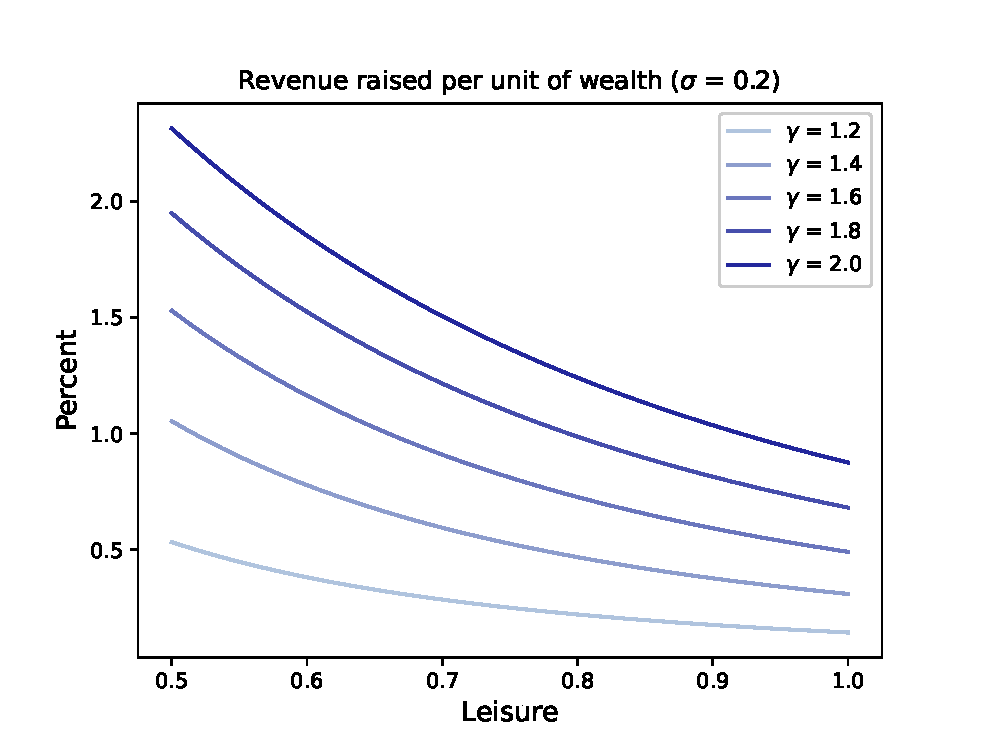
\includegraphics[width=0.49\linewidth]{rev_lgrid}
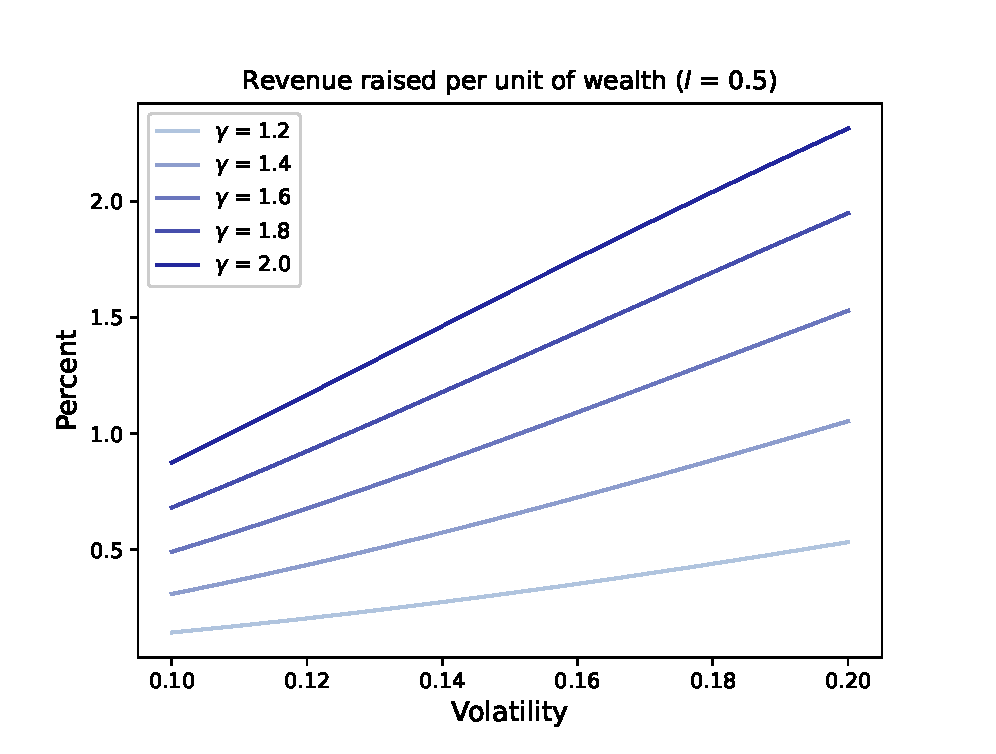
\includegraphics[width=0.49\linewidth]{rev_sig_grid}
\caption{Revenue raised per unit of wealth.}\label{fig:rev}
\end{figure}

Figure \ref{fig:rev} depicts the revenue raised per unit of wealth for various values of $\gamma$. As with Figure \ref{fig:tails} and Figure \ref{fig:tails_log}, on the left-hand side the volatility is fixed at $\sigma=0.2$ and leisure varies, while on the right-hand side the leisure is fixed at $l = \underline{l} = 0.5$ and the volatility varies. As expected, the revenue raised is increasing in volatilty, decreasing in leisure, and tends to zero as the parameters approach logarithmic utility. 

\iffalse
\begin{align*}
0 & = [1 + \alpha(\gamma-1)]\tilde{x}'(\overline{\iota};\tau)/\tilde{x}(\overline{\iota};\tau) + (\gamma-1)(1 - 2\alpha)/\overline{\iota}.
\end{align*}
This simplifies to 
\fi

%\red{The main headache I face is that all of the above expressions assume interior solutions}. 

%under $\overline{\mu}_0 = \rho$, existence is assured. Under logarthmic utility or $\alpha=1/2$, we obtain very intuitive expressions. 

\iffalse
$$
\tau_a + \rho\tau_s(1 - \sigma_c/\sigma) = -\overline{\gamma}(1-\overline{\gamma}) \sigma_c^2. 
$$
we have 
\begin{align*}
\tilde{x}(\overline{\iota}; \tau) & = \frac{1}{\overline{\gamma}}{\left[1 + {\left(\tau_s\overline{\iota} - \overline{\gamma}\sigma^2\overline{\iota}^2/[2\rho] -\tau_a/\rho + 1 - \tau_s\right)}(\overline{\gamma}-1)\right]}
\\ \tilde{x}'(\overline{\iota}; \tau) & = \frac{1}{\overline{\gamma}}{\left(\tau_s - \overline{\gamma}\sigma^2\overline{\iota}/\rho\right)}(\overline{\gamma}-1).
\end{align*}

Using the explicit formula \eqref{x_tilde_func},
the above quadratic becomes
\begin{align*}
Q(\overline{\iota};\tau) & = 1 + [1 + \alpha(\gamma-1)]{\left(\tau_s \overline{\iota}  - \overline{\gamma}\sigma^2\overline{\iota}^2/\rho\right)}\frac{(1-\alpha)}{(1 - 2\alpha)}
\\ & + {\left(\tau_s\overline{\iota} - \overline{\gamma}\sigma^2\overline{\iota}^2/[2\rho] - \tau_a/\rho + 1 - \tau_s\right)}(\overline{\gamma}-1).
\end{align*}

\fi

\textbf{Discussion and special cases.} The optimal taxes in Proposition \ref{linTAXmain} are stated in terms of the share retention function $\overline{\iota}(\tau)$ defined in Lemma \ref{arb_eq}. However, this function is only defined implicitly and the corresponding taxes are only characterized under Assumption \ref{imp_assump}. In this final section I show that Assumption \ref{imp_assump} is satisfied for several common functional forms and that the above algebra simplifies substantially to yield intuitive expressions and further insights. Throughout this section I impose $\overline{\mu}_0 = \rho$, which is satisfied for the parameters considered in Section \ref{PriAg} and ensures that the problem \eqref{initial_prob} simplifies to 
\begin{equation} %\gamma - (\overline{\gamma} - 1) = 1 + \alpha(\gmma-1)
\max_{\overline{\iota} \geq 0} \frac{1 + \alpha(\gamma-1)}{\overline{\gamma}-1}\ln \tilde{x}(\overline{\iota};\tau) + {\left(\frac{1 - 2\alpha}{1 - \alpha}\right)} \ln \overline{\iota}.
\label{initial_prob_simp}
\end{equation}
This objective is globally concave if $\alpha \leq 1/2$, in which case Assumption \ref{imp_assump} is satisfied without any further assumptions on parameters. The first-order condition then characterizes the optimal retention choice and solves %multiplying through by $\tilde{x}(\overline{\iota};\tau) \times \overline{\iota}$
\begin{equation}
0 = \frac{[1 + \alpha(\gamma-1)]}{(\gamma-1)(1 - 2\alpha)}\tilde{x}'(\overline{\iota};\tau)\overline{\iota} + \tilde{x}(\overline{\iota};\tau) =: Q(\overline{\iota};\tau).
\label{quadratic}
\end{equation}
In order to implement the efficient consumption volatility $\sigma_c^*(u_{\textnormal{r}})$, we must choose taxes such that \eqref{quadratic} is satisfied for $\overline{\iota} = \sigma_c^*(u_{\textnormal{r}})/\sigma$ and that the condition in Lemma \ref{IEsig} holds. 

\iffalse
Reminder about following algebra. 
\begin{align*}
0 & = \frac{\rho(1 - 2\alpha)}{(1-\alpha)} + \rho \tau_s \overline{\iota} - \sigma^2 \overline{\iota}^2
\end{align*}
\fi

There are at least two cases in which we obtain substantial simplification. The first case is when utility is logarithmic. Now the quadratic $Q$ in \eqref{quadratic} does not depend on the wealth tax, and the interest tax satisfies $0 = \rho(1 - 2\alpha) + {\left(\rho \tau_s \overline{\iota} - \sigma^2 \overline{\iota}^2\right)}(1-\alpha)$. Using the fact that consumption volatility is now $\sigma_c^*(u_{\textnormal{r}}) = \sigma \alpha (1-\alpha)^{-1}(l^*(u_{\textnormal{r}}))^{-1}$, this implies
\begin{equation}
\tau_s = \frac{\sigma^2/\rho}{(1/\alpha-1)l^*(u_{\textnormal{r}})} + (1 - 1/\alpha)l^*(u_{\textnormal{r}}).
\label{log_system}
\end{equation}
In the earlier, general analysis, I emphasized the distinct conceptual roles played by each tax. One additional insight that emerges clearly in the logarithmic case is that in principle, the tax on interest can assume either sign. Indeed, the expression in \eqref{log_system} is negative for sufficiently small volatility when $\alpha < 1/2$. 

The second case in which the above characterization simplifies is when $\alpha=1/2$.\footnote{This is also the specification chosen by \cite{jones_schumpeterian_2018}, who further assume logarithmic utility.} The optimal share retention now simply maximizes the quadratic $\tilde{x}$ in equation \eqref{x_tilde_func} and implies that $\tau_s = \rho^{-1} \overline{\gamma} \sigma^2 \overline{\iota}$, and so the optimal tax on interest is
\begin{equation} 
\rho \tau_s = \overline{\gamma} \sigma \sigma_c^*(u_{\textnormal{r}})
\label{alpha12}
\end{equation} 
and the tax on wealth becomes
\begin{equation}
\tau_a = \overline{\gamma}^2 \sigma_c^*(u_{\textnormal{r}})^2 - \overline{\gamma} \sigma \sigma_c^*(u_{\textnormal{r}}).
\label{taua12}
\end{equation}
In this case, the tax on interest is unambiguously positive, while the tax on wealth may assume either sign and is negative for all sufficiently small consumption volatility. Further, expressions \eqref{alpha12} and \eqref{taua12} illustrate that in this special case, the optimal taxes on interest and wealth tend to zero smoothly as the degree of idiosyncratic risk vanishes. 


\textbf{Relationship to the literature.} Having derived expressions for the optimal linear taxes and revenue raised for general parameters and for special cases, it is instructive to return once more to a discussion of how these results differ from those in the literature. As mentioned above, the fact that the optimal linear taxation scheme calls for double taxation of capital income, at both the firm and individual level, is reminiscent of the seminal contribution of \cite{albanesi_optimal_2006}, who arrives at such a prescription within a two-period model with an exogenous distribution of physical capital. However, since production occurs only once, the question of how physical capital ought to be distributed among entrepreneurs in the future never arises. Further, if capital could be freely allocated between entrepreneurs, the planner would wish to assign a single entrepreneur to operate the entire capital stock, since doing so would minimize the costs associated with providing incentives in the presence of private information. The primary difference between the current paper and a dynamic extension of \cite{albanesi_optimal_2006} is therefore that business income in the current paper depends on the owner's effort. This assumption, adopted to capture the empirical evidence of \cite{smith_capitalists_2019}, implies that it is simply not possible to reallocate productive resources across entrepreneurs.  In the efficient allocations in this paper, even arbitrarily successful and rich entrepreneurs continue to exert effort as their firm grows, as only they are capable of affecting productivity growth. The above taxes simply ensure that these incentives to retain ownership and exert effort coincide imply that consumption growth coincides with that given in Section \ref{GenEq}. 


\section{Conclusion} \label{Conc}

This paper characterizes a class of constrained efficient allocations in an economy with moral hazard and stochastic growth in business income. There were two principal findings. First, allowing effort to affect output growth rather than levels has important implications for the efficient bearing of risk and hence the degree of inequality in the implied stationary distribution. In dynamic agency models with fixed productivity and standard preferences, agents with high realizations of shocks become too expensive to motivate and so are eventually retired. In contrast, in the model of this paper agents become richer because they experience high productivity growth, and so the benefits of further effort rise along with the costs. In Lemma \ref{lawu} I provide sufficient conditions for this second force to overwhelm the first within a restricted class of contracts and provide numerical evidence that this often holds in the unrestricted optimal contract. In Proposition \ref{RESTdist} I then illustrate the importance of this force by characterizing the associated upper tails of the stationary distributions of consumption and firm size (in terms of output or employment), showing that they do in general differ and that the latter will typically be thicker than the former. 

Second, I derived the optimal linear taxes on capital income and wealth in an environment in which agents may trade shares in their firms or save in a risk-free bond. In this case Proposition \ref{linTAXmain} uncovers a novel role for taxes when productivity depends on unobserved effort: a tax on (personal) capital income alters the incentives of owners to retain ownership of their firm, and hence to exert continued effort to improve productivity. The optimal linear taxation policy in this environment therefore calls for taxes on profits, risk-free interest, and wealth, serving three qualitatively distinct purposes. The tax on profits plays a redistributive role, the tax on risk-free savings provides incentives for retaining equity and continued effort, and the wealth tax serves to implement the efficient level of consumption smoothing.


\bibliography{Business_income}

\appendix

\small

\listoffigures

\section{Recursive analysis}\label{recursiveAPP}

In this section I outline the arguments leading to the Hamilton-Jacobi-Bellman equation. For clarity, define the underlying filtered probability space to be $(\Omega, (\mathcal{F}_t)_{t\geq0},P)$, where $\Omega = C([0,\infty))$, $P$ is the Wiener measure and $\mathcal{F}$ is the $\sigma$-algebra generated by the evaluation maps. In this case the assumption that $l=(l_t)_{t\geq0}$ on $(\Omega, \mathcal{F}, P)$ is progressively measurable is equivalent to the existence of functions $(\tilde{l}_t)_{t\geq0}$ such that $\tilde{l}_t: C([0,t]) \rightarrow \mathbb{R}$ for each $t\geq 0$ and $l_t = \tilde{l}_t((\omega(s))_{0\leq s\leq t})$ almost surely, for all $t \geq0$. These definitions amount to assuming that the choices of the principal and agent at any date are functions of the history of quantities observed up until that date. 

\subsection{Incentive compatibility} \label{ICapp}

For each $l$ define $Z^l_t(\omega) := \omega(t) - \sigma^{-1}\int_{0}^{t}\mu_{\theta}(\tilde{l}_s((\omega(s'))_{0\leq s'\leq s}))ds$ for $\omega \in \Omega$, and note 
that for any $l$ and $l'$ we have $dZ^{l'}_t = dZ^l_t - \sigma^{-1}[\mu_{\theta}(l'_{t}) - \mu_{\theta}(l_{t})]$. We define $P^l$ to be the measure under which $Z^l$ is a Brownian motion on $(\Omega, \mathcal{F}, P^l)$ (see e.g. page 106 of \cite{cvitanic_optimal_2009}). Given the underlying Brownian motion $Z := (Z_t)_{t\geq0}$, we define $\theta$ to be a (strong) solution to $d\theta_t = \sigma \theta_t dZ_t$ and note that
$$
d\theta_t = \sigma \theta_t dZ_t =  \sigma \theta_t {\left(\sigma^{-1}\mu_{\theta}(\tilde{l}(\theta_{\cdot}))dt + dZ_t - \sigma^{-1}\mu_{\theta}(\tilde{l}(\theta_{\cdot}))dt\right)} = \mu_{\theta}(\tilde{l}(\theta_{\cdot}))\theta_t dt + \sigma \theta_t dZ^l_t
$$
and so $(\theta, Z^l, P^l)$ is a (weak) solution to $dX_t = \mu_{\theta}(\tilde{l}(X_{\cdot}))X_t dt + \sigma X_t dW_t$. Finally, we write $\mathbb{E}^l$ for the associated expectation operator on the space of output paths. 

\begin{proof}[Proof of Proposition \ref{contprop}]
For any allocation $(c,l^P)$ and agent strategy $l$, define $V^{c,l} := (V^{c,l}_t)_{t\geq0}$ by
\begin{equation}
V_t^{c,l} := \mathbb{E}^l{\left[\left. \int_{0}^{\infty}\rho e^{-\rho s}u(c_s,l_s) ds \right| \mathcal{F}_t\right]}.
\label{timezero}
\end{equation} %Lemma 3.1 on page 109 of \cite{cvitanic_optimal_2009}
The law of iterated expectations ensures that $V_t^{c,l}$ is a martingale on $(\Omega, \mathcal{F}, P^l)$. The form of the martingale representation theorem given in Lemma 3.1 of \cite{cvitanic_optimal_2009} then implies the existence of $S$ such that $V_t^{c,l} = \rho \sigma \int_{0}^{t} S_sdZ^l_s$ for all $t \geq 0$ almost surely, which gives the first claim. Now consider the case in which the agent adheres to an arbitrary $l$ up until a fixed date $t$ and adheres to $l^P$ thereafter. In this case \eqref{timezero} becomes $V^{c,l}_t := \rho \int_{0}^{t} e^{-\rho s} u(c_s,l_s)ds + e^{-\rho t} U_t$, where $U_t$ is utility if the agent adheres to $l^P$ after $t$. Using $dZ^{l^P}_t = dZ^l_t - \sigma^{-1}[\mu_{\theta}(l^P_{t}) - \mu_{\theta}(l_{t})]$ we have %by the expression \eqref{martrep},
\begin{align*}
dV^l_t & = \rho e^{-\rho t} u(c_t,l_t)dt +  d{\left(e^{-\rho t} U_t\right)}
\\ & = \rho e^{-\rho t} (u(c_t,l_t)dt - U_t)dt + e^{-\rho t} {\left[ \rho(U_t - u(c_t, l_t^P))dt +  \rho\sigma S_tdZ^{l^P}_t\right]}
\\ & = \rho e^{-\rho t}{\left(u(c_t,l_t) - u(c_t, l_t^P) + S_t [\mu_{\theta}(l_t)-\mu_{\theta}(l^P_t)] dt\right)} + \rho \sigma e^{-\rho t} S_tdZ^l_t. %[\sigma dZ_t - \mu(l_t)dt]
\end{align*}
Since $\mathbb{E}^l{\left[ \int_{0}^{t} e^{-\rho s} S_sdZ^l_s \right]} = 0$ for all $t \geq 0$, we have 
\begin{equation}
\mathbb{E}^l[V^l_t] = \hat{V}^l_0 + \rho \mathbb{E}^l{\left[\int_{0}^{t}e^{-\rho s} {\left(S_s\mu_{\theta}(l_s) + u(c_s, l_s) - [S_s\mu_{\theta}(l^P_s) + u(c_s, l^P_s)]\right)}ds \right]}.
\label{punchline}
\end{equation}
Since the expected utility of the agent is $\mathbb{E}^l[ \lim_{t \rightarrow \infty} V^l_t]$, a recommendation $l$ is incentive compatible if and only if it maximizes the integrand in \eqref{punchline} almost surely for all $t \geq 0$, which gives the result. 
\end{proof}

\begin{rmk}
The strengthening of the martingale representation appearing in \cite{cvitanic_optimal_2009} and invoked above appears necessary because $\mathcal{F}$ is the filtration generated by the evaluation maps and is not necessarily equal to the natural filtration associated with $Z^l$.
\end{rmk}

\iffalse
\begin{align*}
dU_t & = \rho{\left(1 - (\overline{c}_t^{1-\alpha}l_t^{\alpha})^{1-\gamma}\right)}U_tdt + \rho \sigma \alpha \frac{(\overline{c}_t^{1-\alpha}l_t^{\alpha})^{1-\gamma}}{(\overline{\mu}_0 - \overline{\mu}_1)l}(1-
df(U_t) & = {\left(\frac{\mu_U}{(1-\overline{\gamma})}+ \frac{\sigma_U^2}{2}\frac{\overline{\gamma}}{(1-\overline{\gamma})^2}\right)}[(1 - \gamma)U_t]^{\frac{1}{1-\overline{\gamma}}}dt +  \frac{\sigma_U}{(1-\overline{\gamma})}[(1 - \gamma)U_t]^{\frac{1}{1-\overline{\gamma}}}dZ_t.
\end{align*}
\fi

\subsection{Laws of motion} \label{laws}

We first assume $\gamma>1$. In this case utility in consumption units and normalized utility are 
\begin{equation}
\begin{aligned}
z_t : & = [(1-\gamma)U_t]^{\frac{1}{1-\overline{\gamma}}} \ \ \ \ \ \ & \ \ \ \ \ \ 
u_t : & = [(1-\gamma)U_t]^{\frac{1}{1-\overline{\gamma}}}\theta_t^{-1}.
\end{aligned}
\label{zut}
\end{equation} 
Recall $\overline{\gamma} := 1 - (1-\gamma)(1-\alpha)$ and $E(l) := \rho\alpha 1_{l<1}/[(1-\alpha)(\overline{\mu}_0 - \overline{\mu}_1)l]$ for any $l \in [\underline{l},1]$, and
\begin{align*}
u(c,l) & = \frac{{\left(c^{1-\alpha}l^{\alpha} \right)}^{1-\gamma}}{1-\gamma} &
u_2(c,l) & = \alpha l^{-1} {\left(c^{1-\alpha}l^{\alpha} \right)}^{1-\gamma} 
\\ \mu_{\theta}(l) & = \overline{\mu}_0 - (\overline{\mu}_0-\overline{\mu}_1)l &
\mu_{\theta}'(l) & = - (\overline{\mu}_0-\overline{\mu}_1)
\end{align*} 
if $l<1$, and $\mu_{\theta}(1) = 0$. Proposition \ref{contprop} shows that we may suppose
\begin{equation}
\begin{aligned}
dU_t & = \rho{\left(U_t - u(c_t,l_t)\right)}dt + \sigma (1-\alpha)E(l_t) {\left(c_t^{1-\alpha}l_t^\alpha\right)}^{1-\gamma}dZ_t.
\end{aligned}
\label{dU1st}
\end{equation} %\frac{(c_t^{1-\alpha}l_t^{\alpha})^{1-\gamma}}{1-\gamma}
We write $c_t = \overline{c}_t[(1-\gamma)U_t]^{\frac{1}{1-\overline{\gamma}}}$, for $\overline{c}_t$ interpreted as consumption per utility in consumption units, and note that $(c_t^{1-\alpha}l_t^{\alpha})^{1-\gamma} = (\overline{c}_t^{1-\alpha}l_t^{\alpha})^{1-\gamma}(1-\gamma)U_t$. The law of motion \eqref{dU1st} becomes $dU_t/U_t = \mu_Udt + \sigma_UdZ_t$ where 
\begin{equation}
\begin{aligned}
\mu_U & = \rho{\left(1 - (\overline{c}_t^{1-\alpha}l_t^{\alpha})^{1-\gamma}\right)} \ \ \ \ \ \ \ & \ \ \ \ \ \ \ 
\sigma_U & = \sigma E(l_t)(\overline{c}_t^{1-\alpha}l_t^{\alpha})^{1-\gamma}(1-\overline{\gamma}).
\end{aligned}
\label{muUsigU}
\end{equation} 
We now wish to derive the laws of motion of $z_t$ and $u_t$ in \eqref{zut}. If $f(U_t) := [(1 - \gamma)U_t]^{\frac{1}{1-\overline{\gamma}}}$ then
\begin{align*}
f'(U_t) : & = \frac{1}{(1-\alpha)}[(1 - \gamma)U_t]^{\frac{\overline{\gamma}}{1-\overline{\gamma}}}
 = \frac{U_t^{-1}}{(1-\overline{\gamma})}f(U_t)
\\ f''(U_t) : & = \frac{\overline{\gamma}}{(1-\alpha)^2}[(1 - \gamma)U_t]^{\frac{\overline{\gamma}}{1-\overline{\gamma}}-1}
= \frac{\overline{\gamma}U_t^{-2}}{(1-\overline{\gamma})^2}f(U_t)
\end{align*} % implies $df(U_t) = (\mu_UU_t f'(U_t)+ (\sigma_U^2/2)U_t^2f''(U_t))dt + f'(U_t)\sigma_UU_tdZ_t$, and so from
and so Ito's lemma and \eqref{muUsigU} imply $dz_t = \mu_zz_tdt + \sigma_zz_tdZ_t$, where 
\begin{equation}
\begin{aligned}
\mu_z & = \frac{\mu_U}{1-\overline{\gamma}}+ \frac{\sigma_U^2}{2}\frac{\overline{\gamma}}{(1-\overline{\gamma})^2} \ \ \ \ \ \ \ & \ \ \ \ \ \ \ 
\sigma_z & = \frac{\sigma_U}{1-\overline{\gamma}}.
\end{aligned}
\label{zlaw0}
\end{equation}
Substituting \eqref{muUsigU} into \eqref{zlaw0} gives
\begin{equation}
\begin{aligned}
\mu_z & = \rho{\left(\frac{1 - (\overline{c}_t^{1-\alpha}l_t^{\alpha})^{1-\gamma}}{1-\overline{\gamma}}\right)} + \frac{\overline{\gamma}\sigma^2}{2} E(l_t)^2 (\overline{c}_t^{1-\alpha}l_t^{\alpha})^{2-2\gamma}
\\ \sigma_z & =  \sigma E(l_t) (\overline{c}_t^{1-\alpha}l_t^{\alpha})^{1-\gamma}.
\end{aligned}
\label{zlaw1}
\end{equation} %In the above we use this with $\sigma_X = \sigma E(l_t) (\overline{c}_t^{1-\alpha}l_t^{\alpha})^{1-\gamma}$ and $\sigma_Y = \sigma 1_{l<1}$.
Since $u_t = z_t/\theta_t$, using Ito's lemma for quotients\footnote{If $dX_t/X_t = \mu_Xdt + \sigma_XdZ_t$ and $dY_t/Y_t = \mu_Ydt + \sigma_YdZ_t$ then $d(X_t/Y_t)/(X_t/Y_t) = (\mu_X - \mu_Y + \sigma_Y^2 - \sigma_X\sigma_Y)dt + (\sigma_X-\sigma_Y)dZ_t$. In the above we use this with $X_t := z_t$ and $Y_t := \theta_t$.} and \eqref{zlaw1} we have $du_t/u_t = \mu_udt + \sigma_u dZ_t$ where
\begin{align*}
\mu_u & = \rho {\left(\frac{1 - (\overline{c}_t^{1-\alpha}l_t^{\alpha})^{1-\gamma}}{1-\overline{\gamma}}\right)} + \frac{\overline{\gamma}\sigma^2}{2} E(l_t)^2(\overline{c}_t^{1-\alpha}l_t^{\alpha})^{2-2\gamma}  - \mu_{\theta}(l_t)
\\ & + \sigma_{\theta}(l_t)^2 - \sigma \sigma_{\theta}(l_t) E(l_t)(\overline{c}_t^{1-\alpha}l_t^{\alpha})^{1-\gamma}
\\ \sigma_u & = \sigma E(l_t)(\overline{c}_t^{1-\alpha}l_t^{\alpha})^{1-\gamma} - \sigma_{\theta}(l_t).
\end{align*}
Factorization and simplification implies that 
\begin{equation}
\begin{aligned}
\mu_u & = \rho {\left(\frac{1 - (\overline{c}_t^{1-\alpha}l_t^{\alpha})^{1-\gamma}}{1-\overline{\gamma}}\right)} + (\overline{\gamma}-1)\frac{\sigma^2}{2} E(l_t)^2(\overline{c}_t^{1-\alpha}l_t^{\alpha})^{2-2\gamma}
\\ & + \frac{\sigma^2_{\theta}(l_t) }{2}(E(l_t)(\overline{c}_t^{1-\alpha}l_t^{\alpha})^{1-\gamma} - 1)^2  - \mu_{\theta}(l_t) + \frac{\sigma^2_{\theta}(l_t) }{2}
%\\ \sigma_u & = \sigma (E(l_t)(\overline{c}_t^{1-\alpha}l_t^{\alpha})^{1-\gamma} - 1_{l_t<1})
\end{aligned}
\label{normlaw}
\end{equation}
which in turn implies \eqref{riskADJ}. The above expressions fail to be well-defined when $\gamma=1$, and so we treat this case separately. We define flow utility to be $u(c,l) = \alpha \ln c + (1-\alpha) \ln l$, and so the analogue of \eqref{zut} is $z_t = \exp(U/(1-\alpha))$ and $u_t = \exp(U/(1-\alpha))\theta^{-1}$. Writing $c_t = \overline{c}_tz_t$, we have $U_t - (1 - \alpha) \ln c_t = - (1 - \alpha) \ln \overline{c}_t$, and so \eqref{dU1st} becomes 
$$
dU_t = \rho{\left(- (1 - \alpha) \ln \overline{c}_t - \alpha \ln l_t\right)}dt + \sigma (1-\alpha)E(l_t) dZ_t =: \mu_Udt + \sigma_UdZ_t.
$$ 
If $f(U_t) := \exp(U/(1-\alpha))$, then $f'(U_t) = (1-\alpha)^{-1}f(U_t)$ and $f''(U_t) = (1-\alpha)^{-2}f(U_t)$, and so from Ito's lemma, we have $dz_t/z_t = \mu_zdt + \sigma_zdZ_t$, where
\begin{equation}
\begin{aligned}
\mu_z & = \frac{\mu_U}{1-\alpha} + \frac{\sigma_U^2}{2(1-\alpha)^2} =-\rho{\left(\ln \overline{c}_t + \frac{\alpha}{1-\alpha} \ln l_t\right)} + \frac{\sigma^2}{2} E(l_t)^2
\\ \sigma_z & = \frac{\sigma_U}{1-\alpha} = \sigma E(l_t).
\end{aligned} %looks 
\label{zlawLOG} 
\end{equation}
Using Ito's lemma for quotients gives $du_t/u_t = \mu_udt + \sigma_udZ_t$, where $\sigma_u = \sigma (E(l_t) - 1_{l_t<1})$ and
\begin{equation}
\begin{aligned} %= -\rho{\left(\overline{c}_t + \frac{\alpha}{1-\alpha} \ln l_t\right)} + \sigma^2 E(l_t)^2/2 - \mu_{\theta}(l_t) + \sigma^21_{l_t<1} - (E(l_t) - 1_{l_t<1})\sigma^2
\mu_u & = -\rho \ln \overline{c}_t - \frac{\rho\alpha}{1-\alpha} \ln l_t + \frac{\sigma^2}{2} E(l_t)^2 - \mu_{\theta}(l_t) + \sigma_{\theta}(l_t)^2 - \sigma^2E(l_t) 
\\ & = -\rho \ln \overline{c}_t - \frac{\rho\alpha}{1-\alpha} \ln l_t - \mu_{\theta}(l_t) + \frac{\sigma_{\theta}(l_t)^2}{2}(E(l_t) - 1)^2 + \frac{\sigma_{\theta}(l_t)^2}{2}.
\end{aligned}
\label{normlawLOG}
\end{equation}


\subsection{Hamilton-Jacobi-Bellman equation} \label{HJB}

Using the original choice variable $(c,l)$, the law of motion of utility \eqref{dU1st}, and the law of motion of productivity \eqref{typeevol}, the Hamilton-Jacobi-Bellman equation is given by 
\begin{equation}
\begin{aligned}
\rho V(U,\theta) & = \max_{\substack{c \geq 0 \\ l \in [\underline{l}, 1]}} \ \theta 1_{l<1} - c + \rho{\left(U - u(c,l)\right)}\frac{\partial V}{\partial U} +
\frac{\sigma^2}{2}{\left((1-\alpha)E(l) {\left(c^{1-\alpha}l^\alpha\right)}^{1-\gamma}\right)}^2\frac{\partial^2V}{\partial U^2}
\\ &  + \mu_{\theta}(l) \theta\frac{\partial V}{\partial \theta} + \frac{\sigma_{\theta}(l)^2}{2}\theta^2\frac{\partial^2V}{\partial \theta^2}+ \sigma (1-\alpha)E(l) {\left(c^{1-\alpha}l^\alpha\right)}^{1-\gamma} \sigma_{\theta}(l)\theta \frac{\partial^2V}{\partial U\partial \theta}.
\label{origHJB}
\end{aligned}
\end{equation}
If $\gamma > 1$, then in terms of the variables $(\overline{c},l)$, where $c = \overline{c}[(1-\gamma)U_t]^{\frac{1}{1-\overline{\gamma}}}$, \eqref{origHJB} becomes
\begin{equation}
\begin{aligned}
\rho V(U,\theta) & = \max_{\substack{\overline{c} \geq 0 \\ l \in [\underline{l}, 1]}} \ \theta 1_{l<1} - \overline{c}[(1-\gamma)U]^{\frac{1}{1-\overline{\gamma}}} + \rho{\left(1 - {\left(\overline{c}^{1-\alpha}l^{\alpha}\right)}^{1-\gamma}\right)}U\frac{\partial V}{\partial U}
\\ & + \frac{\sigma^2}{2}{\left((1-\overline{\gamma})E(l) {\left(\overline{c}^{1-\alpha}l^\alpha\right)}^{1-\gamma}\right)}^2U^2\frac{\partial^2V}{\partial U^2}
 + \mu_{\theta}(l) \theta\frac{\partial V}{\partial \theta} 
 \\ & + \frac{\sigma_{\theta}(l)^2}{2}\theta^2\frac{\partial^2V}{\partial \theta^2} + \sigma (1-\overline{\gamma})E(l){\left(\overline{c}^{1-\alpha}l^{\alpha} \right)}^{1-\gamma}U \sigma_{\theta}(l)\theta \frac{\partial^2V}{\partial U\partial \theta}
\label{CorrectHJB}
\end{aligned}
\end{equation}
where we used $(c^{1-\alpha}l^{\alpha})^{1-\gamma} = (\overline{c}^{1-\alpha}l^{\alpha})^{1-\gamma}(1-\gamma)U$. In the case of logarithmic utility, ($\gamma=1$), in terms of the variables $(\overline{c},l)$, where $c = \overline{c}\exp(U/(1-\alpha))$, \eqref{CorrectHJB} becomes
\begin{equation}
\begin{aligned}
\rho V(U,\theta) & = \max_{\substack{\overline{c} \geq 0 \\ l \in [\underline{l}, 1]}} \ \theta 1_{l<1} - \overline{c}\exp(U/(1-\alpha)) + \rho{\left( - (1-\alpha)\ln \overline{c} - \alpha \ln l\right)}\frac{\partial V}{\partial U}
\\ & + \frac{\sigma^2}{2}(1-\alpha)^2E(l)^2\frac{\partial^2V}{\partial U^2} + \mu_{\theta}(l) \theta\frac{\partial V}{\partial \theta} + \frac{\sigma_{\theta}(l)^2 \theta^2}{2}\frac{\partial^2V}{\partial \theta^2}+ \sigma (1-\alpha)E(l) \sigma_{\theta}(l)\theta \frac{\partial^2V}{\partial U\partial \theta}.
\label{CorrectHJBlog}
\end{aligned}
\end{equation}

\begin{prop} \label{GENhjbMULT}
When $\gamma >1$ the solution to the Hamilton-Jacobi-Bellman equation \eqref{CorrectHJB} is of the form $V(U,\theta) = v(u)\theta$ for some function $v$ solving 
\begin{align*}
\rho v(u) & = \max_{\substack{\overline{c} \geq 0 \\ l \in [\underline{l}, 1]}} \ 1_{l<1} - \overline{c}u + \rho {\left(\frac{1 - (\overline{c}^{1-\alpha}l^{\alpha})^{1-\gamma}}{1-\overline{\gamma}}\right)}uv'(u) + \frac{\overline{\gamma}\sigma^2}{2}E(l)^2{\left(\overline{c}^{1-\alpha}l^{\alpha} \right)}^{2-2\gamma} uv'(u)
\\ & + \mu_{\theta}(l)(v(u) - uv'(u)) + \frac{1}{2}{\left(\sigma E(l){\left(\overline{c}^{1-\alpha}l^\alpha\right)}^{1-\gamma} - \sigma_{\theta}(l)\right)}^2 u^2v''(u).
\end{align*}%E(l) := \frac{\rho \alpha }{(1-\alpha)(\overline{\mu}_0 - \overline{\mu}_1)l}.
\end{prop}

\begin{proof}
Under the change-of-variables $u = u(U,\theta) := [(1-\gamma)U]^{\frac{1}{1-\overline{\gamma}}}\theta^{-1}$, the relevant algebra is
\begin{align*}
u & = [(1-\gamma)U]^{\frac{1}{1-\overline{\gamma}}}\theta^{-1} &
U & = \frac{(u\theta)^{1-\overline{\gamma}}}{1-\gamma} 
\\ \frac{\partial u}{\partial U} & = \frac{1}{1-\alpha}[(1-\gamma)U]^{\frac{\overline{\gamma}}{1-\overline{\gamma}}}\theta^{-1} = \frac{u^{\overline{\gamma}}\theta^{\overline{\gamma}-1}}{1-\alpha}
& \frac{\partial u}{\partial \theta} & = -\frac{u}{\theta}.
\end{align*}
Writing $v(u(U,\theta))\theta = V(U,\theta)$ gives
\begin{align*}
\frac{\partial V}{\partial U} & = \frac{\partial u}{\partial U}v'(u)\theta = \frac{\theta^{\overline{\gamma}} u^{\overline{\gamma}}}{1-\alpha}v'(u)
\\ \frac{\partial V}{\partial \theta} & = v(u) + \frac{\partial u}{\partial \theta}v'(u)\theta = v(u) - uv'(u)
\end{align*}
and 
\begin{align*}
\frac{\partial^2 V}{\partial \theta^2} & = \frac{\partial}{\partial \theta}[v(u) - v'(u) u] = \frac{\partial u}{\partial \theta}[v'(u) - v'(u) - v''(u)u] = v''(u)\frac{u^2}{\theta}
\\ \frac{\partial^2V}{\partial U^2} & = \frac{\theta^{\overline{\gamma}}}{1-\alpha}\frac{\partial}{\partial U}[u^{\overline{\gamma}}v'(u)]
= \frac{\theta^{\overline{\gamma}}}{1-\alpha} \frac{\partial u}{\partial U}[\overline{\gamma} u^{\overline{\gamma}-1}v'(u) + u^{\overline{\gamma}}v''(u)]
= \frac{(u\theta)^{2\overline{\gamma}-2}}{(1-\alpha)^2}[\overline{\gamma} uv'(u) + u^2 v''(u)]\theta
\\  \frac{\partial^2 V}{\partial U \partial \theta} & = \frac{\partial}{\partial U}(v(u) - uv'(u)) = \frac{\partial u}{\partial U}[- uv''(u)] = -\frac{u^{1+\overline{\gamma}}v''(u)}{1-\alpha}\theta^{\overline{\gamma}-1}.
\end{align*} 
Substitution into \eqref{CorrectHJB} gives
\begin{align*}
\rho v(u)\theta & = \max_{\substack{\overline{c} \geq 0 \\ l \in [\underline{l}, 1]}} \ (1_{l<1} - \overline{c}u) \theta + \rho {\left(1 - {\left(\overline{c}^{1-\alpha}l^{\alpha} \right)}^{1-\gamma} \right)}U\frac{\theta^{\overline{\gamma}} u^{\overline{\gamma}}}{1-\alpha}v'(u)
\\ & + \frac{\sigma^2}{2}E(l)^2(1-\overline{\gamma})^2 {\left(\overline{c}^{1-\alpha}l^{\alpha} \right)}^{2-2\gamma}U^2\frac{(u\theta)^{2\overline{\gamma}-2}}{(1-\alpha)^2}[\overline{\gamma} uv'(u) + u^2 v''(u)]\theta
\\ & + \mu_{\theta}(l)\theta(v(u) - uv'(u)) + \frac{\sigma_{\theta}(l)^2 \theta }{2}v''(u)u^2 - \sigma \sigma_{\theta}(l)E(l){\left(\overline{c}^{1-\alpha}l^\alpha\right)}^{1-\gamma} v''(u)u^{1+\overline{\gamma}}(1-\gamma)U\theta^{\overline{\gamma}}. %(1-\alpha)
\end{align*}
Dividing by $\theta$ and using $u^{1-\overline{\gamma}} = (1-\gamma)U\theta^{\overline{\gamma}-1}$ and \eqref{Efunc} then gives
\begin{align*}
\rho v(u) & = \max_{\substack{\overline{c} \geq 0 \\ l \in [\underline{l}, 1]}} \ 1_{l<1} - \overline{c}u + \rho {\left(\frac{1 -  {\left(\overline{c}^{1-\alpha}l^\alpha\right)}^{1-\gamma}}{1-\overline{\gamma}}\right)}uv'(u) + \frac{\sigma^2}{2}E(l)^2{\left(\overline{c}^{1-\alpha}l^\alpha\right)}^{2-2\gamma}[\overline{\gamma} uv'(u) + u^2 v''(u)] 
\\ & + \mu_{\theta}(l) (v(u) - uv'(u)) + \frac{\sigma_{\theta}(l)^2}{2}u^2v''(u) - \sigma \sigma_{\theta}(l)E(l) {\left(\overline{c}^{1-\alpha}l^{\alpha} \right)}^{1-\gamma}u^2 v''(u)
\end{align*}
which simplifies as claimed upon factorization. 
\end{proof}

We have the following analogue in the case of logarithmic utility. The proof is almost identical to that of Proposition \ref{GENhjbMULT} and so omitted.

\begin{prop} \label{GENhjbMULTlog}
When utility is logarithmic, the solution to the Hamilton-Jacobi-Bellman equation \eqref{CorrectHJBlog} is of the form $V(U,\theta) = v(u)\theta$ for some function $v$ solving 
\begin{align*}
\rho v(u) & = \max_{\substack{\overline{c} \geq 0 \\ l \in [\underline{l}, 1]}} \ 1_{l<1} - \overline{c}u + \rho {\left(-\ln \overline{c} - \frac{\alpha \ln l}{1-\alpha}\right)}uv'(u) + \frac{\sigma^2}{2}E(l)^2 uv'(u)
\\ & + \mu_{\theta}(l)(v(u) - uv'(u)) + \frac{\sigma^2}{2}{\left(E(l) - 1_{l<1}\right)}^2 u^2v''(u).
\end{align*}
\end{prop}

\subsection{Restricted value and policy functions} \label{restAPP}

\begin{proof}[Proof of Proposition \ref{propREST}]
Using Proposition \ref{GENhjbMULT}, substituting the form $v \equiv \overline{v}_{\textnormal{r}}(l)u + \underline{v}_{\textnormal{r}}(l)$ and equating the linear and constant parts gives $\underline{v}_{\textnormal{r}}(l) = 1_{l<1}/(\rho - \mu_{\theta}(l))$ and $\overline{v}_{\textnormal{r}}(l)$ solves
\begin{equation}
\begin{aligned}
\rho \overline{v}_{\textnormal{r}}(l) & = \max_{\substack{\overline{c} \geq 0}} \ -\overline{c} + \rho{\left(\frac{1 - (\overline{c}^{1-\alpha}l^{\alpha})^{1-\gamma}}{1-\overline{\gamma}} \right)}\overline{v}_{\textnormal{r}}(l) + \frac{\overline{\gamma}\sigma^2}{2} E(l)^2 {\left(\overline{c}^{1-\alpha}l^{\alpha} \right)}^{2-2\gamma} \overline{v}_{\textnormal{r}}(l).
\label{HJBconstant}
\end{aligned}
\end{equation}
Note that the right-hand side is concave in $\overline{c}$ and diverges to $-\infty$ for any $\overline{v}_{\textnormal{r}}(l) < 0$. Consequently, if a solution to \eqref{HJBconstant} exists then the optimal consumption level satisfies a first-order condition and we therefore arrive at the pair of equations
\begin{align*}
\rho \overline{v}_{\textnormal{r}}(l) & = -\overline{c} + \rho{\left(\frac{1 - (\overline{c}^{1-\alpha}l^{\alpha})^{1-\gamma} }{1-\overline{\gamma}}\right)}\overline{v}_{\textnormal{r}}(l) + \frac{\overline{\gamma}\sigma^2}{2} E(l)^2{\left(\overline{c}^{1-\alpha}l^{\alpha}\right)}^{2-2\gamma}\overline{v}_{\textnormal{r}}(l)
 \\ 0 & = -\overline{c} - \rho(\overline{c}^{1-\alpha}l^{\alpha})^{1-\gamma}\overline{v}_{\textnormal{r}}(l) + (2-2\overline{\gamma})\frac{\overline{\gamma}\sigma^2}{2}E(l)^2{\left(\overline{c}^{1-\alpha}l^{\alpha} \right)}^{2-2\gamma}\overline{v}_{\textnormal{r}}(l).
\end{align*}
Equating the two expressions for $\overline{c}$ and dividing by $\overline{v}_{\textnormal{r}}(l)$ gives a quadratic in $x := (\overline{c}^{1-\alpha}l^{\alpha})^{1-\gamma}$
\begin{align*}
\rho (1 - x) + (2 - 2\overline{\gamma})\frac{\overline{\gamma} \sigma^2}{2} E(l)^2x^2 & = \frac{\rho(1 - x)}{1-\overline{\gamma}} + \frac{\overline{\gamma} \sigma^2}{2} E(l)^2 x^2
\end{align*} 
which simplifies to the claimed quadratic. Further, for the maintained assumption $\overline{\gamma} \geq 1$, this quadratic has only one positive solution (and hence only one sensible solution), which corresponds to the solution to \eqref{HJBconstant}. Using the fact that $c_t = \overline{c}u_t\theta_t = \overline{c}z_t$ for $z_t$ as defined in Appendix \ref{laws}, the expression \eqref{zlaw1} then gives
\begin{align*} 
\rho \overline{v}_{\textnormal{r}}(l)  & = -\overline{c} + \rho {\left(\frac{1 - x}{1-\overline{\gamma}}\right)}\overline{v}_{\textnormal{r}}(l) + \frac{\overline{\gamma}\sigma^2}{2} E(l)^2x^2 \overline{v}_{\textnormal{r}}(l) = -\overline{c} + \mu_c(l) \overline{v}_{\textnormal{r}}(l).
\end{align*}
which rearranges to give $\overline{v}_{\textnormal{r}}(l)$. Finally, note that $\overline{v}_{\textnormal{r}}(l)$ solves $\rho \overline{v} = T(\overline{v})$, where 
\begin{align*}
T(\overline{v}) = \max_{\substack{\overline{c} \geq 0}} \ - \overline{c} + \rho {\left(\frac{ (\overline{c}^{1-\alpha}l^{\alpha})^{1-\gamma} - 1}{\overline{\gamma} - 1} \right)}\overline{v} + \frac{\overline{\gamma}\sigma^2}{2} E(l)^2 {\left(\overline{c}^{1-\alpha}l^{\alpha} \right)}^{2-2\gamma} \overline{v} .
\end{align*}
Since $\overline{\gamma}, \gamma >1$, $T$ is increasing in $l$ whenever $\overline{v}$ is negative since it is the pointwise maxima of increasing functions. The fixed-point will then be increasing in $l$ provided the right-hand side is convex in $\overline{v}$, which is true as it is the pointwise maxima of affine functions. 
\end{proof}

%The above shows that here is unique solution o $T(v) = v \rho$. 

The case of logarithmic utility corresponds to $\overline{\gamma}=1$ and so the expressions in Propostion \ref{propREST} are not well-defined. In this case we define $V(U,\theta) = v(u)\theta$ as before but now set $u = \exp(U/(1-\alpha))\theta^{-1}$. %The same guess-and-verify procedure as above gives the following. 

\begin{lemma}\label{RESTlogLEMMA}
In the case of logarithmic utility the restricted-action value and policy functions are 
\begin{equation}
\begin{aligned}
v_{\textnormal{r}}(u;l) & = \frac{1_{l<1}}{\rho-\mu_{\theta}(l)} - \frac{1}{\rho}\exp{\left(\sigma^2E(l)^2/[2\rho]\right)}l^{-\frac{\alpha}{1-\alpha}}u
\\ c_{\textnormal{r}}(u;l) & = \exp{\left(\sigma^2E(l)^2/[2\rho]\right)}l^{-\frac{\alpha}{1-\alpha}}u.
\label{RESTlog}
\end{aligned}
\end{equation}
\end{lemma}

\begin{proof}
Using Proposition \ref{GENhjbMULTlog}, substituting the form $v_{\textnormal{r}} \equiv \overline{v}_{\textnormal{r}}(l)u + \underline{v}_{\textnormal{r}}(l)$ and equating the linear and constant parts gives $\underline{v}_{\textnormal{r}}(l) = 1/(\rho - \mu_{\theta}(l))$ and $\overline{v}_{\textnormal{r}}(l)$ solves
\begin{align*}
\rho \overline{v}_{\textnormal{r}}(l) & = \max_{\substack{\overline{c} \geq 0}} \ - \overline{c} + \rho {\left(-\ln \overline{c} - \frac{\alpha \ln l}{1-\alpha}\right)}\overline{v}_{\textnormal{r}}(l) + \frac{\sigma^2}{2}E(l)^2\overline{v}_{\textnormal{r}}(l).
\end{align*}
The first-order condition gives $\overline{c} = \rho[-\overline{v}_{\textnormal{r}}(l)]$, and the above becomes $\ln (-\rho\overline{v}_{\textnormal{r}}(l)) = - \alpha(1-\alpha)^{-1} \ln l + \sigma^2E(l)^2/[2\rho]$, which rearranges as claimed.
\end{proof}


\section{Stationary distribution proofs} \label{distproofs}
\subsection{Planner preferences} \label{planPREFapp}

Defining $\Omega' := \mathbb{R} \times \Theta \times \{E,W\}$, aggregate consumption, output and aggregate labor assigned \text{to} entrepreneurs at any date $t\geq0$ are then,
\begin{align*}
C_t & := e^{-\rho_Dt}\underline{C}_t + \rho_D\int_{0}^{t}e^{-\rho_D (t-T)} C^T_tdT
\\ \underline{C}_t  & := \int_{\Omega'}\mathbb{E}[c^{v,\theta,i}_t]\Phi(d\omega), \ \ \ \ \ C^T_t := \sum_{i=E,W}\eta_i \mathbb{E}[c^{T,i}_t]
\\ Y_t & := e^{-\rho_Dt}\underline{Y}_t + \rho_D\int_0^te^{-\rho_D (t-T)} Y^T_tdT
\\ \underline{Y}_t & := \int_{\Omega'}\mathbb{E}[F(\theta^{v,\theta,i}_t,L^{v,\theta,i}_{t})]\Phi(d\omega), \ \ \ \ \ Y^T_t := \eta_E\mathbb{E}[F(\theta^{T,E}_t,L^{T,E}_t)]
\\ L_t & := e^{-\rho_Dt}\underline{L}_t + \rho_D\int_{0}^{t}e^{-\rho_D(t-T)}L^T_tdT
\\ \underline{L}_t & := \int_{\Omega}\mathbb{E} [L^{v,\theta,E}_{t}]\Phi(d\omega), \ \ \ \ \ L^T_t = \eta_E\mathbb{E}[L^{T,E}_t].
\end{align*}
Since the planner only weights workers, the flow utility at date $t$ is 
\begin{align*}
U_t & := e^{- \rho_D t}\underline{U}_t + \rho_D\int_{0}^{t}e^{-\rho_D(t-T)} U^T_tdT
\\ \underline{U}_t & := \int_{\Omega'} \mathbb{E}[u(c^{v,\theta,i}_t,l^{v,\theta,i}_t)]\Phi(d\omega), \ \ \ \ \ U^T_t := (1-\eta_E)\mathbb{E}[u(c^{T,W}_t,l^{T,W}_t)]
\end{align*} 

\begin{lemma}\label{planpreflemma}
The preferences of the planner are represented by the function $\int_0^{\infty} e^{-\rho_S t}U_tdt$.
\end{lemma}

\begin{proof}
Proceeding from first principles, the objective of the planner is
\begin{align*}
U^P & = \int_{\Omega'}\mathbb{E}{\left[\int_{0}^{\infty} e^{- \rho t}u(c^{v,\theta,i}_t,l^{v,\theta,i}_t)dt\right]} \Phi(d\omega)
\\ & + \rho_D\int_{0}^{\infty}e^{-\rho_S T} (1-\eta_E) \mathbb{E}{\left[\int_{T}^{\infty} e^{- \rho(t-T)}u(c^{T,W}_t,l^{T,W}_t)dt\right]} dT
\\ & = \int_{0}^{\infty} e^{- \rho_S t}\int_{\Omega'} e^{- \rho_D t}\mathbb{E}[u(c^{v,\theta,i}_t,l^{v,\theta,i}_t)]dt \Phi(d\omega) dt
\\ & + \rho_D (1-\eta_E)\int_{0}^{\infty} e^{- \rho_S t} \int_{0}^{t}e^{-\rho_D (t-T)}\mathbb{E}[u(c^{T,W}_t,l^{T,W}_t)]dTdt
\end{align*} %$e^{-\rho T}e^{- (\rho+\rho_D) (t-T)} = e^{-\rho T}e^{- \rho(t-T)}e^{-\rho_D (t-T)} = e^{- \rho t}e^{-\rho_D (t-T)}$
where I used $e^{-\rho_S T}e^{- \rho (t-T)} = e^{- \rho_S t}e^{-\rho_D (t-T)}$, which gives the result upon simplification. 
\end{proof}

\subsection{Reduction to principal-agent problem}

The Lagrangian associated with the relaxed planner's problem is
\begin{align*}
\mathcal{L} & = \int_0^{\infty} e^{-\rho_S t} {\left(U_t + \lambda_R{\left[Y_t - C_t + \lambda_L(\overline{L} - L_t)\right]} \right)}dt.
\end{align*}
Using the above expressions we may then expand this as 
\begin{align*}
\mathcal{L} %& = \lambda_R\lambda_L\overline{L} + \int_0^{\infty} e^{-\rho t} {\left(\underline{U}_t + \lambda_R{\left[\underline{Y}_t - \lambda_L\underline{L}_t - \underline{C}_t\right]} \right)}dt
%\\ & + \int_0^{\infty} e^{-\rho_S t} \rho_D\int_{0}^{t}e^{-\rho_D (t-T)}{\left(U^T_t + \lambda_R{\left[Y^T_t  - \lambda_LL^T_t - C^T_t\right]} \right)}dTdt
& = \lambda_R\lambda_L\overline{L} + \int_0^{\infty} e^{-\rho t} {\left(\underline{U}_t + \lambda_R{\left[\underline{Y}_t - \lambda_L\underline{L}_t - \underline{C}_t\right]} \right)}dt
\\ & + \rho_D\int_0^{\infty}e^{-\rho_S T} \int_{T}^{\infty} e^{- \rho (t-T)}{\left(U^T_t + \lambda_R{\left[Y^T_t  - \lambda_LL^T_t - C^T_t\right]} \right)}dtdT
\end{align*}
where I again used $e^{-\rho_S T}e^{- \rho (t-T)} = e^{- \rho_St}e^{-\rho_D(t-T)}$ and interchanged the order of integration. For any $T \geq0$ I write $\mathcal{A}_T$ for the subset of allocations associated with agents born at time $T$, and $\mathcal{A}^{IC}_T$ for the associated incentive compatible allocations. For a given multiplier the task of the planner choosing quantities for agents born at date $T$ is 
\begin{align*}
\max_{\mathcal{A}^{IC}_T} \ & \int_{0}^{\infty} e^{-\rho t} (U^T_t + \lambda_R[Y^T_t - \lambda_LL^T_t - C^T_t])dt.
\end{align*}
Since the planner weights only workers, he is forced to provide all agents with a common utility level. For entrepreneurs the problem becomes $\max_U \ U + \lambda_RV(U,\overline{Z}(\lambda_L))$, where $V$ is the value function of the principal in Section \ref{PriAg}. The problem of the planner facing a given generation is therefore
\begin{align*}
V^G_{\lambda} & = \max_{\substack{U_E,U_W < 0 \\ U_E \geq U_W}} \ \eta_E{\left(U_E + \lambda_R\overline{Z}(\lambda_L)V(U_E\overline{Z}(\lambda_L)^{\overline{\gamma}-1},1)\right)} + (1-\eta_E) {\left(U_W - \lambda_R[(1-\gamma)U_W]^{\frac{1}{1-\overline{\gamma}}}\right)}
%\\ & = \max_{U < 0} \ U + \eta_E\lambda_R\overline{Z}(\lambda_L)v([(1-\gamma)U]^{\frac{1}{1-\overline{\gamma}}}/\overline{Z}(\lambda_L)) - (1-\eta_E) \lambda_R[(1-\gamma)U]^{\frac{1}{1-\overline{\gamma}}}
\\ & = \max_{y \geq 0} \ \overline{Z}(\lambda_L)^{1-\overline{\gamma}}\frac{y^{1-\overline{\gamma}}}{1-\gamma} + \lambda_R\overline{Z}(\lambda_L)[\eta_E v(y) - (1-\eta_E) y].
\end{align*}
The task of the planner is to therefore pick a value of $y := [(1-\gamma)U]^{\frac{1}{1-\overline{\gamma}}}/\overline{Z}(\lambda_L)$ and to then follow the recommendations of the principal with normalized utility given by $y$. 

\iffalse
\subsection{Reduction to principal-agent problem without Lagrangian}

Recall that given an initial distribution $\Phi$, the relaxed planning problem is defined to be 
\begin{align*}
V^R(\Phi) = \max_{A \in \mathcal{A}^{IC}} \ \int_0^{\infty} e^{-\rho_S t} U_t & dt
\\ \int_0^{\infty}e^{-\rho_S t}(C_t - Y_t)dt & \leq 0
\\ \int_0^{\infty}e^{-\rho_S t}(L_t - \overline{L})dt & \leq 0.
\end{align*}
It does not appear to be necessary to construct a Lagrangian in order to solve the above, as a first principles argument ought to suffice. For the moment, let us ignore the labor resource constraint and focus solely on the goods resource constraint. Expanding the above objective and constraint into contributions from separate generations then yields 
\begin{align*}
V^R(\Phi) = \max_{A \in \mathcal{A}^{IC}} \ & \int_0^{\infty} e^{-\rho_S t} {\left(e^{- \rho_D t}\underline{U}_t + \rho_D\int_0^te^{-\rho_D(t-T)} U^T_tdT \right)} dt
\\ \int_0^{\infty}e^{-\rho_S t}e^{-\rho_Dt}(\underline{C}_t - \underline{Y}_t)dt
& + \int_0^{\infty}e^{-\rho_S t}\rho_D\int_0^te^{-\rho_D (t-T)} (C^T_t - Y^T_t)dTdt \leq 0.
\end{align*}
In any solution to the relaxed planner problem, conditional on choosing an amount of utility $(U^T_t)_{t\geq0}$ assigned to a generation born at date $T$, the planner will choose consumption and leisure recommendations to minimize the discounted (at rate $\rho_S$) cost of delivering this lifetime utility. This is a necessary condition for an allocation to solve the above, for otherwise the planner could choose another allocation that delivers the same amount of utility to that generation and costs strictly less, allowing the planner to reallocate such resources to a different generation and so increase their objective. It will be instructive to view the problem of the planner as choosing a level of utility for a particular generation, and subsequently minimizing the discounted cost of providing that level of utility to each generation.

The problem may then be written 
\begin{align*}
\max_{A \in \mathcal{A}^{IC}} \int_0^{\infty} e^{-\rho t} \underline{U}_tdt + \rho_D\int_0^{\infty}& e^{-\rho_S T} {\left(\int_T^{\infty} e^{- \rho (t-T)}U^T_tdt\right)}dT
\\ \int_0^{\infty} e^{-\rho t} {\left[\underline{Y}_t - \underline{C}_t\right]} dt
 + \rho_D\int_0^{\infty} & e^{-\rho_S T} {\left(\int_T^{\infty} e^{- \rho (t-T)}[Y^T_t - C^T_t]dt\right)}dT \leq 0
\end{align*}
Now introduce some notation for lifetime utility and expected lifetime costs. Define 
\begin{align*}
\hat{\underline{U}} & =  \int_0^{\infty} e^{-\rho t} \underline{U}_tdt 
& \hat{U}^T & = \int_T^{\infty} e^{- \rho (t-T)}U^T_tdt
\\ \hat{\underline{C}} & =  \int_0^{\infty} e^{-\rho t} \underline{C}_tdt 
& \hat{C}^T & = \int_T^{\infty} e^{- \rho (t-T)}C^T_tdt
\\ \hat{\underline{Y}} & =  \int_0^{\infty} e^{-\rho t} \underline{Y}_tdt 
& \hat{Y}^T & = \int_T^{\infty} e^{- \rho (t-T)}Y^T_tdt.
\end{align*}
Consequently the relaxed planner problem may be written 
\begin{align*}
\max_{A \in \mathcal{A}^{IC}} \ \hat{\underline{U}} + \rho_D\int_0^{\infty}& e^{-\rho_S T} \hat{U}^TdT
\\ \hat{\underline{Y}} - \hat{\underline{C}} + \rho_D\int_0^{\infty} & e^{-\rho_S T} {\left(\hat{Y}^T - \hat{C}^T\right)}dT \leq 0
\end{align*}
The point of allowing one to trade intertemporally at price $\rho_S$ and hire workers at a competitive wage $w$ is that we now have a single constraint, which functions as a kind of budget constraint for the planner planner. When the planner can trade in this manner, the cost of providing lifetime utility $U$ to a newborn entrepreneur is given by $-V(U,\overline{Z}(w)) = -V(U\overline{Z}(w)^{\overline{\gamma}-1},1)\overline{Z}(w)$, which is will be convex in $U$ provided $V(U,1)$ is concave in $U$. The computed value function is typically concave, but it is not clear if this is guaranteed by the assumptions in the main text. However, this is not an impediment to the invocation of Lagrangian techniques provided we allow the planner to resort to ex-ante lotteries. If they are able to do this, then they will wish to treat all generations the same. For this reason for the recursive analysis in the main text we may need to replace the value function $V(U,1)$ with the ``concavification'' given by
\begin{align*}
V^*(U) := & \max_{N,(p_i,U_i)_{i=1}^N} \ \sum_{i=1}^N p_i V(U_i,1)
\\ U & = \sum_{i=1}^N p_i U_i 
\end{align*}
which corresponds to the value function of a planner who owes an agent $U$ units of lifetime utility and who is permitted to run a lottery prior to contracting with the agent. Further, $V^*$ is concave regardless of the shape of $V$. To see this, consider any two $U_1$ and $U_2$ and $\alpha \in (0,1)$, and denote by $(p_{i1},U_{i1})_{i=1}^{N_1}$ and $(p_{i2},U_{i2})_{i=1}^{N_2}$ the probabilities and utility levels satisfying $\sum_{i=1}^{N_1} p_{i1} U_{i1} = U_1$ and $\sum_{i=1}^{N_2} p_{i2} U_{i2} = U_2$. Then we have 
\begin{align*}
\alpha U_1 + (1-\alpha)U_2 & = \alpha \sum_{i=1}^{N_1} p_{i1} U_{i1} + (1-\alpha)\sum_{i=1}^{N_2} p_{i2} U_{i2}
\end{align*}
and so by the definition of $V^*$ we have 
\begin{align*}
V^*(\alpha U_1 + (1-\alpha)U_2) & \geq \alpha\sum_{i=1}^{N_1} p_{i1} V(U_{i1},1) + (1-\alpha)\sum_{i=1}^{N_2} p_{i2} V(U_{i2},1)
\\ & = \alpha V^*(U_1) + (1 - \alpha) V^*(U_2).
\end{align*}
\fi

\iffalse
\begin{align*}
\max_U \ U + \lambda_R\overline{Z}(\lambda_L)V(U\overline{Z}(\lambda_L)^{\overline{\gamma}-1},1) & = \max_U \ U + \lambda_R\overline{Z}(\lambda_L)v([(1-\gamma)U]^{\frac{1}{1-\overline{\gamma}}}/\overline{Z}(\lambda_L))
%\\ & = \max_{x \geq 0} \ \frac{x^{1-\overline{\gamma}}}{1-\gamma} + \lambda_R\overline{Z}(\lambda_L)v(x/\overline{Z}(\lambda_L))
\\ & = \lambda_R\overline{Z}(\lambda_L)\max_{u \geq 0} \ \frac{1}{\lambda_R\overline{Z}(\lambda_L)^{\overline{\gamma}}}\frac{u^{1-\overline{\gamma}}}{1-\gamma} + v(u).
\end{align*}
Each multiplier therefore corresponds to a choice of $u$ and hence lifetime utility $\overline{Z}(\lambda_L)u$.
Lagrange's theorem implies there exists $\lambda := (\lambda_R, \lambda_L)$ such that the optimal allocation solves
$$
V_{\lambda}(\Phi) := \max_{A \in \mathcal{A}^{IC}} \int_{0}^{\infty} e^{-\rho t}{\left(U_t + \lambda_R{\left[Y_t - C_t + \lambda_L{\left(\overline{L} - L_t\right)}\right]}\right)}dt
$$
In view of expressions given in Appendix \ref{planPREFapp}, for a given multiplier the task of the planner when choosing quantities relevant for agents born at date $T$ is given by 
\begin{align*}
V^G_\lambda = \max_{\mathcal{A}^{IC}_T} \ & \int_{0}^{\infty} e^{-\rho t} (U^T_t + \lambda_R[Y^T_t - C^T_t + \lambda_L(\overline{L} - L^{T,E}_t)])dt
\end{align*}
where 
\begin{align*}
C^T_t & := \int_{0}^{t}e^{-\rho_D (t-T)} \sum_{i=E,W}\eta_i \mathbb{E}[c^{T,i}_t]dT &
Y^T_t & := \int_{0}^{t}e^{-\rho_D (t-T)} \sum_{i=E,W}\eta_i\mathbb{E}[F(\theta^{T,i}_t, L^{T,i}_t)]dT 
\\ L^T_t & := \int_{0}^{t}e^{-\rho_D(t-T)} \eta_E\mathbb{E}[L^{T,E}_t]dT  &
U^T_t & := \int_{0}^{t}e^{-\rho_D(t-T)} \sum_{i=E,W}\eta_i\mathbb{E}[u(c^{T,i}_t,l^{T,i}_t)]dT.
\end{align*} 
\fi

\subsection{Kolmogorov forward equation for joint law}\label{Kolm}
The Kolmogorov forward equation gives the evolution of the joint density of utility and productivity. The following shows that the summary measure given in Definition \ref{summary_m} solves a version of the Kolmogorov forward equation for a single variable. For a proof of the following, see Appendix \ref{Kolm}.
\begin{lemma} \label{summarylemma}
If $(u_t,\theta_t)_{t\geq0}$ evolves according to $(du_t,d\theta_t) = (\mu_uu_t dt + \sigma_uu_tdZ_t, \mu_{\theta} \theta_t dt + \sigma_{\theta}\theta_t dZ_t)$ for some $\mu_u,\sigma_u,\mu_{\theta}$ and $\sigma_{\theta}$, then $m$ solves the ordinary differential equation
\begin{equation}
0 = -(\rho_D-\mu_{\theta}(u)) m(u) -  [(\mu_u(u) + \sigma_\theta(u)\sigma_u(u))um(u)]' + \frac{1}{2}[\sigma^2_u(u)u^2m(u)]''.
\label{ODEsummary}
\end{equation}
\end{lemma} 

The homogeneity of the policy functions and the exponential growth of productivity ensure that we need only solve for the density of a single variable, referred to as the summary measure.\footnote{I owe the following observation to a discussion with Hengjie Ai.}

\begin{proof}[Proof of Lemma \ref{summarylemma}]
The process $(\theta_t,u_t)_{t\geq0}$ is a diffusion process driven by the same Brownian motion and so away from $(\theta_0,u_0)$ the joint density satisfies the Kolmogorov forward equation
\begin{align*}
\frac{\partial }{\partial t} [\Phi(\theta,u,t)] & = - \rho_D \Phi(\theta,u,t) - \mu_{\theta}(u)\frac{\partial}{\partial \theta}[\theta\Phi(\theta,u,t)] -\frac{\partial}{\partial u}[\mu_u(u)\Phi(\theta,u,t)] \\ & \ + \frac{\sigma_{\theta}(u)^2}{2}\frac{\partial^2}{\partial \theta^2}[\theta^2\Phi(\theta,u,t)] + \frac{\partial^2}{\partial \theta \partial u}[\theta \sigma_{\theta}(u)\sigma_u(u)\Phi(\theta,u,t)]
 + \frac{1}{2}\frac{\partial^2}{\partial u^2}[\sigma_u^2(u)\Phi(\theta,u,t)].
\end{align*}
First note that the stationary distribution $\overline{\Phi}$ satisfies $\lim_{\theta \rightarrow \infty }\theta \overline{\Phi}(\theta,u) = 0$ for all $u$, since we have assumed that $\rho_D > \mu_{\theta}(l)$ for all $l \in [\underline{l},1]$. For any smooth $f$ vanishing at zero and satisfying $\lim_{\theta \rightarrow \infty }\theta f(\theta) = 0$, integration by parts gives $\int_{0}^{\infty} \theta f'(\theta)d\theta = [\theta f(\theta)]_{\theta=0}^{\infty} - \int_{0}^{\infty}  f(\theta)d\theta = - \int_{0}^{\infty}  f(\theta)d\theta$ and $\int_{0}^{\infty} \theta f''(\theta)d\theta =  - \int_{0}^{\infty} f'(\theta)d\theta = 0$. Recalling the definition $m(u,t) := \int_{0}^{\infty}\theta\Phi(\theta,u,t)d\theta$ and interchanging orders of integration, it follows that for all $(u,t)$ we have the following simplifications
\begin{align*}  %= -\mu \int_{0}^{\infty}[\theta\Phi(\theta,u,t)]d\theta
\mu_{\theta}(u) \int_{0}^{\infty}\theta\frac{\partial}{\partial \theta}[\theta\Phi(\theta,u,t)]d\theta & = -\mu_{\theta}(u) m(u,t)
\\  -\int_0^{\infty}\theta\frac{\partial}{\partial u}[\mu_u(u)\Phi(\theta,u,t)] d\theta & = -\frac{\partial}{\partial u} [\mu_u(u) m(u,t)]
\\ \frac{\sigma_{\theta}^2(u)}{2}\int_{0}^{\infty}\theta\frac{\partial^2}{\partial \theta^2}[\theta^2\Phi(\theta,u,t)]d\theta & = 0 
\\  \int_{0}^{\infty}\theta\frac{\partial^2}{\partial \theta \partial u}[\theta \sigma_u(u)\Phi(\theta,u,t)]d\theta & =
- \frac{\partial}{\partial u}[\sigma_u(u) m(u,t)]
\\ \int_{0}^{\infty}\theta\frac{\partial^2}{\partial u^2}[\sigma_u^2(u)\Phi(\theta,u,t)]d\theta
& = \frac{\partial^2}{\partial u^2}[\sigma_u^2(u)m(u,t)].
\end{align*}
Interchanging the order of integration, the multi-dimensional forward equation implies
\begin{align*}
\frac{\partial }{\partial t} \int_{0}^{\infty}\theta\Phi (\theta,u,t)d\theta & = - \rho_D\int_{0}^{\infty}\theta\Phi(\theta,u,t)d\theta - \mu_{\theta}(u) \int_{0}^{\infty}\theta\frac{\partial}{\partial \theta}[\theta\Phi(\theta,u,t)]d\theta
\\ & - \frac{\partial}{\partial u}\int_{0}^{\infty}\theta \mu_u(u)\Phi(\theta,u,t) d\theta + \frac{\sigma_{\theta}(u)^2}{2}\int_{0}^{\infty}\theta\frac{\partial^2}{\partial \theta^2}[\theta^2\Phi(\theta,u,t)]d\theta
\\ & + \sigma_{\theta}(u)\int_{0}^{\infty}\theta\frac{\partial^2}{\partial \theta \partial u}[\theta \sigma_u(u)\Phi(\theta,u,t)]d\theta
 + \frac{1}{2}\int_{0}^{\infty}\theta\frac{\partial^2}{\partial u^2}[\sigma_u(u)^2\Phi(\theta,u,t)]d\theta
\end{align*}
which is equivalent to 
$$
\frac{\partial m}{\partial t} = -(\rho_D - \mu_{\theta}(u))m(u,t) - \frac{\partial}{\partial u}[(\mu_u(u) + \sigma_{\theta}(u)\sigma_u(u))m(u,t)] + \frac{1}{2}\frac{\partial^2}{\partial u^2}[\sigma^2_u(u)m(u,t)].
$$
Setting the partial derivative with respect to time to zero then gives \eqref{ODEsummary}.
\end{proof}

\subsection{Restricted-action distributions} \label{restDISTsect}
For convenience the following recalls a well-known fact regarding killed diffusion processes.
\begin{lemma} \label{genLEMMA}
The stationary distribution of a stochastic process that dies at rate $\delta_X$, is injected at some $\overline{X} > 0$, and otherwise evolves according to $dX_t = \mu_XX_tdt + \sigma_XX_t dZ_t$, is given by 
$$
f(x) = A x^{\alpha^+_X-1}_X1_{x \leq \overline{X}} + B x^{\alpha^-_X-1}1_{x > \overline{X}}
$$
where $\alpha^{\pm}_X =  \overline{\mu}_X/\sigma_X^2 \pm  \sqrt{(\overline{\mu}_X/\sigma_X^2)^2+2\delta_X/\sigma_X^2}$, the constants $A$ and $B$ are chosen such that the density is continuous and integrates to unity, and $\overline{\mu}_X = \mu_X - \sigma_X^2/2$ for brevity.
\end{lemma}
\begin{proof}[Proof of Proposition \ref{RESTdist}] The proof proceeds by combining Lemma \ref{genLEMMA} with the policy functions for consumption given in Proposition \ref{propREST}. From \eqref{zlaw1} we have $dc_t = \mu_cc_tdt + \sigma_cc_t dZ_t$, where
\begin{align*}
\mu_c & = \frac{\rho(1 - x)}{1-\overline{\gamma}} + \frac{\overline{\gamma}\sigma^2}{2}E(l)^2x^2  &
\sigma_c & = \sigma E(l)x
\end{align*}
where $(\overline{\gamma} - 1) (\overline{\gamma} - 1/2) \sigma^2 E(l)^2 x^2 = \rho(1 - x)$. Using the defining equation for $x(l)$ we then have 
\begin{align*}
\mu_c & = \frac{\rho(1 - x)}{1-\overline{\gamma}} + \frac{\overline{\gamma}\sigma^2}{2}E(l)^2x^2 = (1 - \overline{\gamma})\frac{\sigma^2}{2}E(l)^2x^2.
\end{align*}
Consequently, $\mu_c - \sigma_c^2/2 = -\overline{\gamma} \sigma^2 E(l)^2x^2/2$. Using Lemma \ref{genLEMMA} the tails are then
\begin{align*}
\alpha^{\pm}_c &  =  \overline{\mu}_X/\sigma_X^2 \pm  \sqrt{{\left(\overline{\mu}_X/\sigma_X^2\right)}^2 + 2\delta_X/\sigma_X^2}   =  -\frac{\overline{\gamma}}{2}  \pm  \sqrt{ \frac{\overline{\gamma}^2}{4} + \frac{2\rho_D}{\sigma^2E(l)^2x^2}} 
\end{align*}
which simplifies as claimed using the defining quadratic for $x$. 
\end{proof}

\iffalse
Using the defining equation for $x$ in $0 = \sigma^2E(l)^2(\overline{\gamma}-1)(\overline{\gamma}-1/2)x^2 + \rho x - \rho$, we have 
\begin{align*}
\frac{2\rho_D}{\sigma^2E(l)^2x^2} & =  \frac{\rho_D(\overline{\gamma}-1)(2\overline{\gamma}-1)}{\rho (1-x)}
\end{align*}
and so the above expressions simplify to
\begin{align*}
\alpha^{\pm}_c &  =  -\frac{\overline{\gamma}}{2}  \pm  \sqrt{ \frac{\overline{\gamma}^2}{4} + \frac{2\rho_D}{\sigma^2E(l)^2x^2}} 
\\ &  =  -\frac{\overline{\gamma}}{2}  \pm \sqrt{ \frac{\overline{\gamma}^2}{4} + \frac{\rho_D(\overline{\gamma}-1)(2\overline{\gamma}-1)}{\rho (1-x)}} 
\\ &  =  -\frac{\overline{\gamma}}{2}  \pm \frac{\overline{\gamma}}{2}\sqrt{ 1 + \frac{4\rho_D(\overline{\gamma}-1)(2\overline{\gamma}-1)}{\rho (1-x)}} 
\end{align*}
and so 
$$
\alpha^{\pm}_c (l) = -\frac{\overline{\gamma}}{2}  \pm  \frac{\overline{\gamma}}{2}\sqrt{1 + \frac{4\rho_D(1 - 1/\overline{\gamma}) (2-1/\overline{\gamma})}{\rho(1-x(l))}} 
$$ 
\fi

\section{Additional figures} \label{sec:add_figures}

In this appendix I compute several figures that complement those given in the main text. 

\subsection{Principal-agent problem}

Figure \ref{fig:l_c_log} computes analogues of Figure \ref{fig:l_c} and Figure \ref{fig:law_u} when utility is logarithmic, which corresponds to the limit $\gamma \rightarrow 1$.

\begin{figure}[H] %[H]
\centering
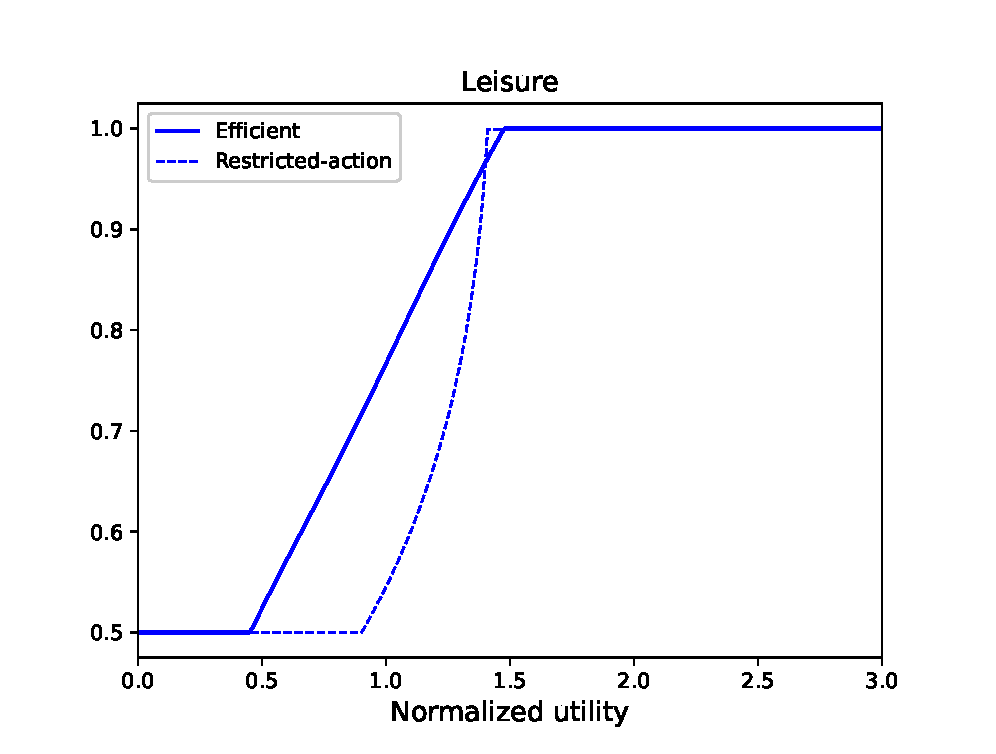
\includegraphics[width=0.49\linewidth]{leisure_log}
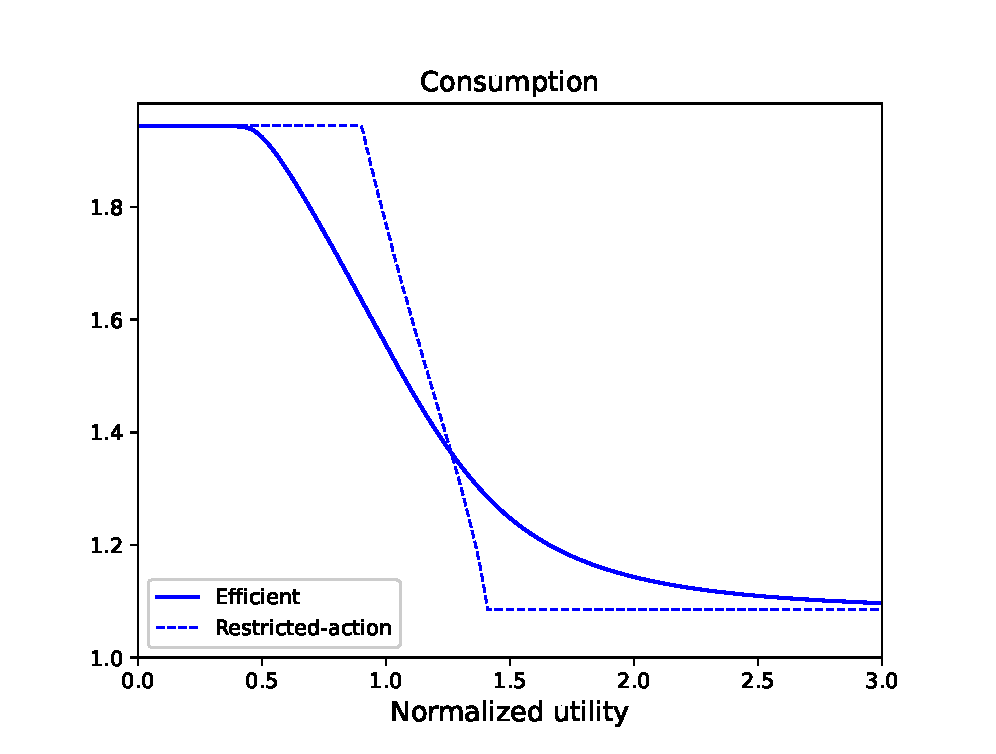
\includegraphics[width=0.49\linewidth]{consumption_log}
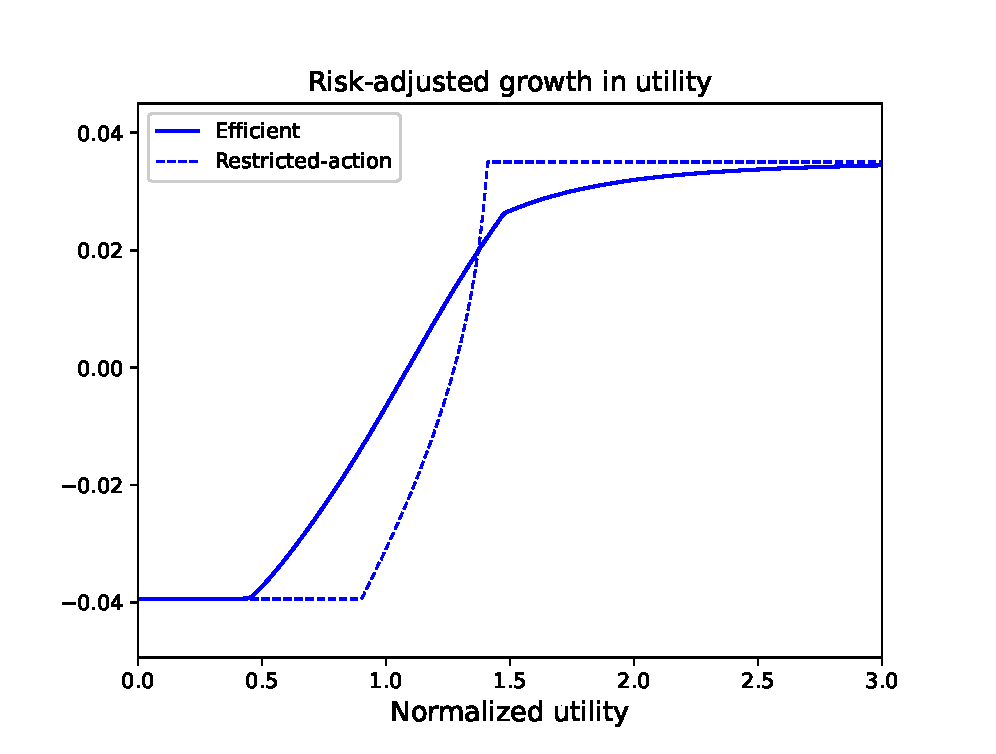
\includegraphics[width=0.49\linewidth]{risk_adj_log}
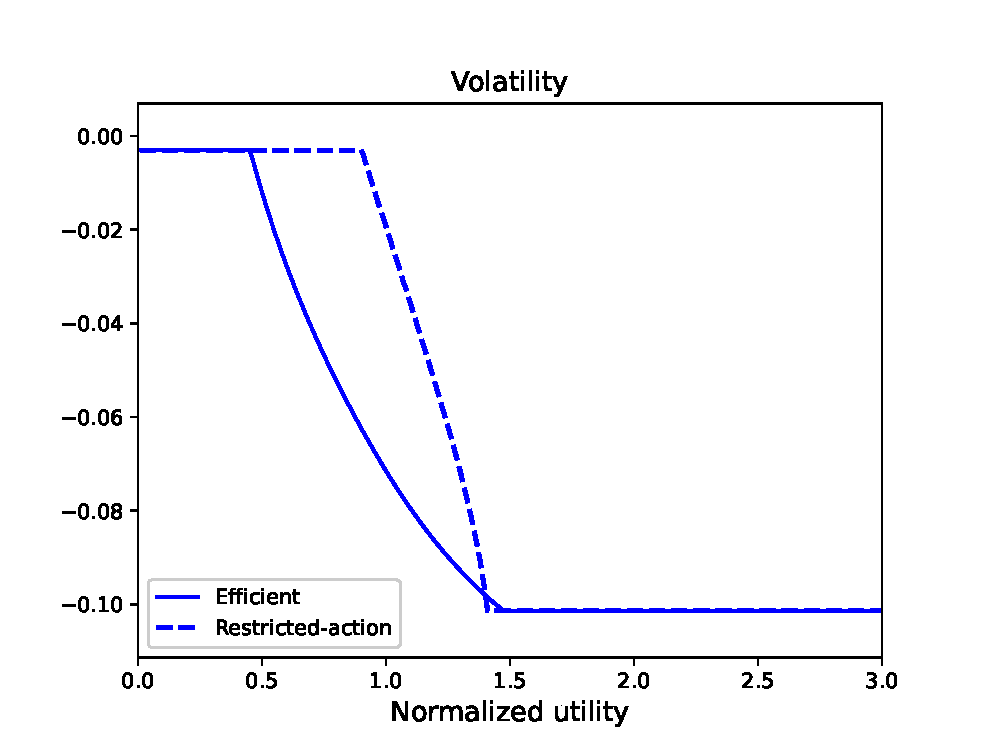
\includegraphics[width=0.49\linewidth]{sig_u_log}
\caption{Policy functions and dynamics of normalized utility for logarithmic utility.}
\label{fig:l_c_log}
\end{figure}

\subsection{Stationary efficient allocation}

Figure \ref{fig:tails_log} computes the tails of the stationary distributions for consumption and firm size, as a function of both volatility and effort. 

\begin{figure}[H]
\centering
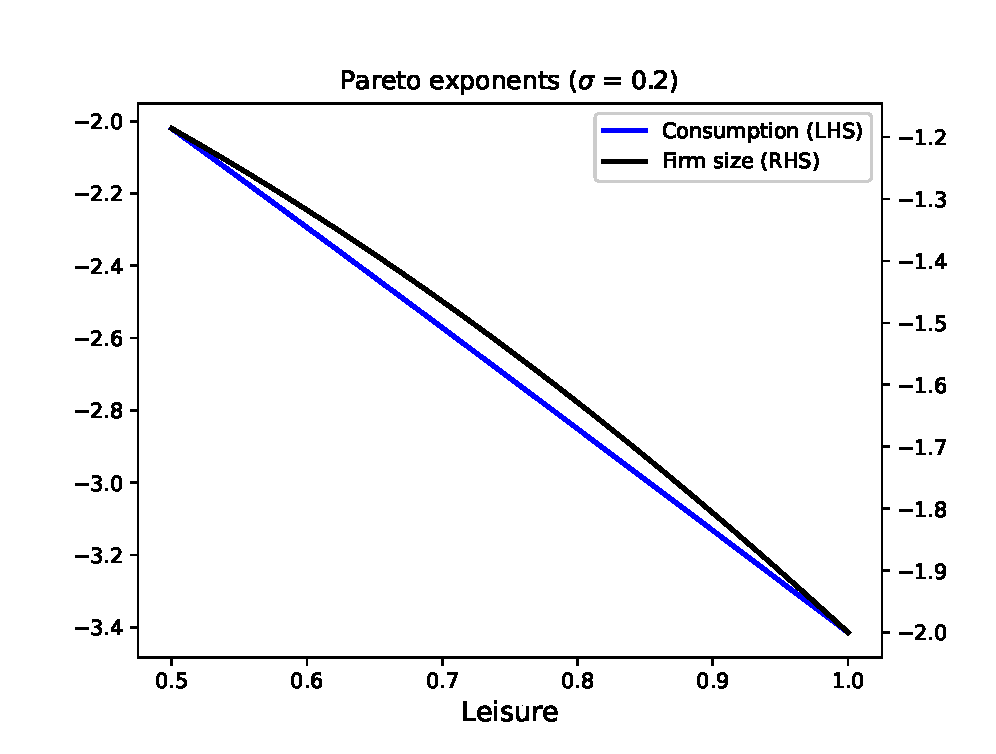
\includegraphics[width=0.49\linewidth]{tails_log}
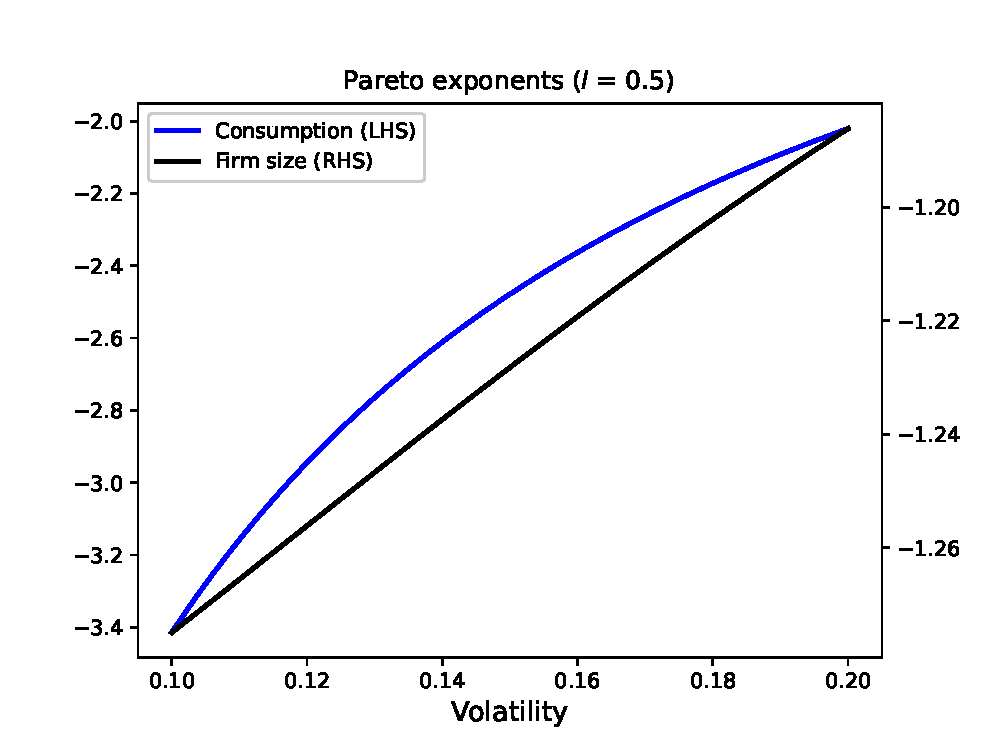
\includegraphics[width=0.49\linewidth]{tails_sig_log}
\caption{Tail parameters for firm size and consumption with logarithmic utility}\label{fig:tails_log}
\end{figure}


\section{Optimal linear taxes}

\subsection{Discrete-time analogue} \label{discCE} 

The continuous-time agent problem is the limit of discrete-time environments of the following form:
\begin{itemize}
\item At $t$ the agent has wealth $a_t$. She places $b_t$ in a risk-free bond earning after-tax return $(1-\tau_s)(r+\rho_D)$ and uses the remaining $\iota_t := a_t - b_t$ to purchase shares at price $p_t$. 
\item At $t+\Delta$ shareholders receive after-tax dividends $\Delta (1-\tau_d)\overline{Z}\theta_t$ from the firm's output produced over $[t,t+\Delta]$. By $t+\Delta$ productivity has grown to $\overline{Z}\theta_{t+\Delta}$ and the price is $p_{t+\Delta}$.
\item Wealth at $t+\Delta$ is holdings of bonds and stocks, plus flow dividends minus consumption,
\begin{equation}
\begin{aligned}
a_{t+\Delta} & = a_t + \textnormal{interest} - \textnormal{consumption} + \textnormal{dividends} + \textnormal{capital gains} - \textnormal{wealth tax}
\\ & = a_t + (1-\tau_s)(r + \rho_D)\Delta b_t - \Delta c_t + \Delta (1-\tau_d)\overline{Z} \theta_t x_t + (1-\tau_{cg}) (p_{t+\Delta} - p_{t})x_t - \tau_a\Delta a_t
\\ & = a_t + \Delta {\left[[(1-\tau_s)(r + \rho_D) - \tau_a] a_t -  c_t +  [(1-\tau_d)\overline{Z} \theta_t/p_t - (1-\tau_s)(r + \rho_D)]\iota_t\right]} \\ & + (p_{t+\Delta}/p_t-1)(1-\tau_{cg})\iota_t.
\end{aligned}
\label{approx}
\end{equation} %where I substituted $x_t = \iota_t/p_t$ and  $b_t = a_t - p_t x_t$.
\end{itemize}
The approximate law of motion for the price is $p_{t+\Delta}/p_t - 1 = \mu_{\theta}(l)\Delta + \sigma \sqrt{\Delta} dX$ where $dX$ is mean zero i.i.d. across time and assumes values $\pm 1$. Substituting into \eqref{approx} and taking limits as $\Delta \rightarrow 0$
\begin{align*}
%a_{t+\Delta} & = a_t + \Delta {\left[(1-\tau_s)(r + \rho_D) a_t -  c_t +  [(1-\tau_d)\overline{Z}\theta_t/p_t + (1-\tau_{cg})\mu_{\theta}(l) - (1-\tau_s)(r + \rho_D)]\iota_t\right]}
%\\ & + \sigma \sqrt{\Delta} (1-\tau_{cg})\iota_tdX 
da_t & = {\left[[(1-\tau_s)(r + \rho_D) - \tau_a]a_t - c_t + {\left((1-\tau_d)\overline{Z}\theta_t/p_t + (1-\tau_{cg})\mu_{\theta}(l_t) - (1-\tau_s)(r + \rho_D)\right)} \iota_t \right]}dt
\\ & + \sigma (1-\tau_{cg})\iota_t dZ_t.
\end{align*}
If $\hat{l}(u) \equiv \hat{l}$ then $p_t = (1-\tau_d)\overline{Z}\theta_t/[r + \rho_D - \mu_{\theta}(\hat{l})]$, and so 
$$
da_t = {\left[[(1-\tau_s)(r + \rho_D) - \tau_a]a_t - c_t + {\left(\tau_s (r + \rho_D) + (1- \tau_{cg})\mu_{\theta}(l_t) - \mu_{\theta}(\hat{l})\right)}\iota_t\right]}dt + \sigma (1-\tau_{cg})\iota_t dZ_t
$$
which is the expression implied by \eqref{linearP3} and \eqref{return}. 

\subsection{Transfers and debt policy} \label{debt_pol}

In this section I specify the transfers and debt policy necessary to support the optimal linear taxes characterized in Proposition \ref{linTAXmain}. First note that
\begin{equation}
\overline{Z} = (1-\beta)Z{\left(\frac{\rho_D\eta_E}{\rho_D - \mu_{\theta}(l)} \right)}^{-\beta}\overline{L}^{\beta} = \frac{(\rho_D - \mu_{\theta}(l))}{\eta_E \rho_D}(1-\beta)Y
\label{zequil2}
\end{equation}
where $Y$ denotes aggregate output. The utility that agents obtain is then a solution to
$$ 
Y = Z{\left(\frac{\rho_D\eta_E}{\rho_D - \mu_{\theta}(l)} \right)}^{1-\beta}\overline{L}^{\beta} = {\left(\frac{\rho_D \eta_E\overline{c}_{\textnormal{r}}(l)}{\rho_D - \mu_c(l)} + 1 - \eta_E\right)}[(1-\gamma)U]^{\frac{1}{1-\overline{\gamma}}} =: \kappa(l)[(1-\gamma)U]^{\frac{1}{1-\overline{\gamma}}}.
$$
The right-hand side of the above is the sum of the stationary level of worker consumption and entrepreneur consumption when the latter begins at $\overline{c}_{\textnormal{r}}(l)[(1-\gamma)U]^{\frac{1}{1-\overline{\gamma}}}$ and grows at $\mu_c$. Steady-state utility at birth in consumption units is $[(1-\gamma)U]^{\frac{1}{1-\overline{\gamma}}} = Y/\kappa(l)$ and so by Lemma \ref{valCOEFF} the initial wealth of entrepreneurs must be 
$$
a_E = \rho^{-1} [(1-\gamma)U]^{\frac{1}{1-\overline{\gamma}}}x(l)^{\frac{\overline{\gamma}}{1-\overline{\gamma}}}l^{-\frac{\alpha}{1-\alpha}} = \rho^{-1}Yx(l)^{\frac{\overline{\gamma}}{1-\overline{\gamma}}}l^{-\frac{\alpha}{1-\alpha}}  \kappa(l)^{-1}.
$$
Further, we have by definition $\overline{c}_{\textnormal{r}}(l) = x(l)^{\frac{1}{1-\overline{\gamma}}}l^{-\frac{\alpha}{1-\alpha}}$. Consequently, we can write 
\begin{equation}
\kappa(l) = \frac{\rho_D \eta_E x(l)^{\frac{1}{1-\overline{\gamma}}}l^{-\frac{\alpha}{1-\alpha}}}{\rho_D - (1-\overline{\gamma})\sigma^2 E(l)^2 x(l)^2/2} + 1 - \eta_E.
\label{kappa}
\end{equation}
To obtain utility $Y/\kappa(l)$ workers require $(Y/\rho)\kappa(l)^{-1}$ units of wealth. They obtain $\beta Y/\rho$ from their labor income, and so the value of transfers must be $T = (Y/\rho)(1/\kappa(l) - \beta)$. Since the entrepreneurs also earn wage income the after-tax value of their firm at birth must equal $(Y/\rho){\left(x(l)^{\frac{\overline{\gamma}}{1-\overline{\gamma}}}l^{-\frac{\alpha}{1-\alpha}}/\kappa(l) - \beta\right)}$. The value of the firm is $(1-\tau_d)\overline{Z}/(\rho - \mu_{\theta}(l))$, and so using \eqref{zequil2} the tax on dividends is
\begin{align*}
\frac{(1-\tau_d)(\rho_D - \mu_{\theta}(l))}{(\rho - \mu_{\theta}(l))\eta_E \rho_D}(1-\beta)Y & = \frac{Y}{\rho}{\left( \frac{x(l)^{\frac{\overline{\gamma}}{1-\overline{\gamma}}}l^{-\frac{\alpha}{1-\alpha}}}{\kappa(l)} - \beta\right)}
\\ \tau_d & = 1 - \frac{\rho_D(\rho - \mu_{\theta}(l))}{\rho(\rho_D - \mu_{\theta}(l))}{\left( \frac{x(l)^{\frac{\overline{\gamma}}{1-\overline{\gamma}}}l^{-\frac{\alpha}{1-\alpha}}-\kappa(l)}{\kappa(l)(1-\beta)} + 1\right)}\eta_E.
\end{align*}
The revenue from the dividends tax minus the flow transfers as a fraction of output $Y$ is then
\begin{align*}
\tau_d(1-\beta) - \rho_D(1-\eta_E)\frac{T}{Y} & = 1 - \beta - \frac{\rho_D(\rho - \mu_{\theta}(l))}{\rho(\rho_D - \mu_{\theta}(l))}{\left( \frac{x(l)^{\frac{\overline{\gamma}}{1-\overline{\gamma}}}l^{-\frac{\alpha}{1-\alpha}}}{\kappa(l)} - \beta\right)}\eta_E
\\ & - \frac{\rho_D}{\rho}(1-\eta_E){\left(\frac{1}{\kappa(l)} - \beta \right)}.
\end{align*}
The interest payments paid by the government as a fraction of profits $(1-\beta)Y$ must then be 
\begin{equation}
1 - \frac{\rho_D}{\rho}{\left[\frac{(\rho - \mu_{\theta}(l))}{(\rho_D - \mu_{\theta}(l))}{\left( \frac{x(l)^{\frac{\overline{\gamma}}{1-\overline{\gamma}}}l^{-\frac{\alpha}{1-\alpha}}-\kappa(l)}{\kappa(l)(1-\beta)} + 1\right)} \eta_E + (1-\eta_E){\left(\frac{1/\kappa(l) - \beta}{1-\beta} \right)} \right]}.
\label{interestDY}
\end{equation}
To demystify the above it is useful to consider some special cases. If $\beta = 0$ and $\eta_E = 1$, then
\begin{align*}
\tau_d & = 1 - \frac{\rho_D(\rho - \mu_{\theta}(l))}{\rho(\rho_D - \mu_{\theta}(l))}{\left( \frac{x(l)^{\frac{\overline{\gamma}}{1-\overline{\gamma}}}l^{-\frac{\alpha}{1-\alpha}}-\kappa(l)}{\kappa(l)} + 1\right)} = 1 - \frac{\rho_D(\rho - \mu_{\theta}(l))}{\rho(\rho_D - \mu_{\theta}(l))} {\left(\frac{\rho_D - \mu_c}{\rho_D}\right)}.
\end{align*} 
In the absence of any discounting across generations we have $\rho_D = \rho$, and hence $\tau_d = \mu_c/\rho$, and so by Corollary \ref{colREVENUEmain} the dividends tax takes the opposing sign of the taxes raised on capital and wealth. Further, if $\alpha = 0$ then we have $\kappa(\underline{l}) = 1$ and $x(\underline{l}) = 1$, and so
\begin{align*}
\tau_d & = 1 - \frac{\rho_D(\rho - \mu_{\theta}(\underline{l}))}{\rho(\rho_D - \mu_{\theta}(\underline{l}))}
 = \frac{(\rho_D - \rho)\mu_{\theta}(\underline{l}))}{\rho(\rho_D - \mu_{\theta}(\underline{l}))}.
\end{align*}
This expression is negative, and so in this case the government is running a surplus, the proceeds of which are used to fund a subsidy to firm profits. At birth, the investors take possession of the firms (since the entrepreneurs need not retain any equity). The debt held by the government (i.e. the negative of the amount issued) as a fraction of output is
\begin{align*}
\frac{1}{\rho-\rho_D}{\left(1 - \frac{\rho_D}{\rho}{\left[\frac{(\rho - \mu_{\theta}(l))}{(\rho_D - \mu_{\theta}(l))}  \right]}\right)} = -\frac{1}{\rho}{\left(1 - \frac{\rho_D}{\rho_D - \mu_{\theta}(l)}\right)}
\end{align*} %agents
In this case the value of each firm at birth is $Y/\rho$. To understand who holds the debt in this economy, note that the government holds $(Y/\rho)\rho_D/(\rho_D - \mu_{\theta}(l))$ and so the investors must hold the negative of this quantity. Since the investors own all of the firms in the economy, they earn all (after-tax) profits, and so after purchasing new firms with a flow of $\rho_DY/\rho$ government bonds their net revenues every instant are 
\begin{align*}
& \ \ \ (1-\tau_d)Y - \frac{\rho_D}{\rho}Y - \frac{Y}{\rho}\frac{\rho_D}{(\rho_D - \mu_{\theta}(l))}(\rho - \rho_D)
\\ & = \frac{Y}{\rho}{\left[\rho - \rho_D + (\rho - \rho_D) \frac{\mu_{\theta}(l)}{(\rho_D - \mu_{\theta}(l))} - \frac{\rho_D}{(\rho_D - \mu_{\theta}(l))}(\rho - \rho_D)\right]} = 0
\end{align*}
as expected.


\section{Competitive versus signaling equilibria} \label{eqcompare}

As noted in the main text, an earlier draft of this paper derived optimal taxes for a different solution concept, in which the price of each entrepreneur's business was assumed to be independent of the portfolio choices of the agent. Such an allocation could be expected to prevail if the portfolio choices of the entrepreneur were unobservable. In this case, taxes on interest income are necessary for the existence of a rational expectations equilibria with nonzero effort, because if the price of the firm is equal to the present discounted value of output and savings are untaxed, then the owner has no incentive to retain ownership and investors rationally expect zero effort.

It is always possible to choose taxes so that the first-order conditions of the entrepreneur are consistent with the consumption and leisure choices in the optimal restricted-action allocations. However, this ``competitive'' notion of equilibrium is fragile, as these first-order conditions are not always sufficient to solve the consumer's problem and non-existence of equilibrium may arise.\footnote{The possibility of non-existence was erroneously overlooked in previous drafts, and so some of the allocations did not depict true competitive equilibria.} Essentially, the possibility of varying consumption, effort and the amount of shares retained leads the maximand in the consumer problem to be non-concave, and so the first-order conditions of the consumer problem only characterize the equilibrium when agency frictions are sufficiently large to discourage ``double deviations'' (in which the entrepreneur sells shares and reduces effort jointly). For this reason, the equilibrium notion adopted in the main text is of a ``signaling'' type, in which the portfolio choice of the entrepreneur is observable to investors and affects both the price of the firm and the incentives for continued effort. For the market structure in the main text, no further assumptions are necessary to ensure existence of equilibria. 

However, although the expressions for taxes (and the robustness of existence) differ across the two equilibrium notions, the amount of tax revenue raised per unit of wealth does not (whenever both allocations exist). Further, the roles played by taxes are qualitatively the same across the two allocations. For this reason I outline the competitive equilibrium taxes in this appendix. 

\begin{defn} \label{conPROBlin}
Given an interest rate $r$, linear taxes $\tau = (\tau_d,\tau_s,\tau_{cg},\tau_a)$, and expectations of effort exerted governed by $(\hat{l}_t)_{t\geq0}$, the problem of an entrepreneur with firm size $\theta$ and wealth $a$ is
\begin{align*}
V(a,\theta) = \max_{\overline{c},l,\overline{\iota}} & \ \mathbb{E}^l{\left[\int_{0}^{\infty}\rho e^{-\rho t}u(\overline{c}_ta_t,l_t)dt\right]}
\\ da_t & = [(1-\tau_{s})(r + \rho_D) - \tau_a - \overline{c}_t]a_tdt + \overline{\iota}_t a_tdR_t(l_t;\hat{l}_t)
\\ d\theta_t & = \mu_{\theta}(l_t)\theta_t dt + \sigma_{\theta}(l_t) \theta_t dZ_t
\\ (a_0,\theta_0) & = (a,\theta).
\end{align*}
\end{defn}
Notice that the homotheticity of preferences ensures that the sole effect of a constant linear profits tax is to scale the initial wealth of the agent state-by-state, leaving the portfolio and effort decisions unaffected. The notion of equilibrium adopted here is of a standard rational expectations type: agents optimize, markets clear, and expectations are consistent with individual incentives. 

\begin{defn} \label{SME}
Given constant linear taxes $\tau$, a competitive stock market equilibrium consists of wages $w$, effort expectations governed by $\hat{l}$, and policy functions $(\overline{c},l,\overline{\iota}) = (\overline{c}_t,l_t,\overline{\iota}_t)_{t\geq0}$ for consumption, leisure, and investment, such that the following hold:
\begin{itemize}
\item The policy functions $(\overline{c},l,\overline{\iota})$ solve the entrepreneur's problem in Definition \ref{conPROBlin} given the expectations for leisure $\hat{l}$ and taxes $\tau$. 
\item The outside investors break even in expectation, or $l_t = \hat{l}$ for all $t\geq0$ almost surely. 
\item The markets for goods and labor clear every instant. 
\item The government budget constraint is satisfied. 
\end{itemize}
A stationary competitive stock market equilibrium is one in which the cross-sectional distributions of wealth and firm size are constant over time. 
\end{defn} 
The transfers to workers and the level of government debt will be set so that the goods market clears. The first observation relevant for our characterization is that if expectations are constant, then for for a given choice of effort, the entrepreneur's problem becomes a standard portfolio problem of Merton-Samuelson type and admits a homogeneous solution. However, for an arbitrary set of taxes and prices, the first-order conditions need not characterize the solution since the drift in the law of motion for wealth is not concave in $(c, l, \overline{\iota})$. I will first proceed under the assumption that such first-order conditions characterize the solution to the individual problem, and then derive sufficient conditions to ensure that this approach is valid in terms of deep parameters of the model. 

% However, the first-order conditions may be shown to characterize the optimum for sufficiently high volatility.

\begin{lemma}\label{MertonSam}
When the first-order approach is valid and effort expectations are constant, the choice of leisure is constant, and the policy functions for consumption and investment are of the form $c(a) = \overline{c}a$ and $\iota(a) = \overline{\iota}a$ for some constants $\overline{c}$ and $\overline{\iota}$, where $(\overline{c}, l)$ solve 
\begin{equation}
\begin{aligned}
\frac{\overline{c}}{\rho} & = \frac{(1 - \tau_{cg})\mu_{\theta}(l) - \mu_{\theta}(\hat{l}) + \tau_s\rho}{E(l)\overline{\gamma}\sigma^2(1-\tau_{cg})}
\\ \frac{\rho - \overline{\gamma}\overline{c}}{1-\overline{\gamma}} & = (1-\tau_s)\rho - \tau_a  + \frac{((1 - \tau_{cg})\mu_{\theta}(l) - \mu_{\theta}(\hat{l}) + \tau_s\rho)^2}{2\overline{\gamma}\sigma^2(1-\tau_{cg})^2}
 \end{aligned}
\label{3by34}
\end{equation}
and investment is given by
$$
\overline{\iota} = \frac{(1 - \tau_{cg})\mu_{\theta}(l) - \mu_{\theta}(\hat{l}) + \tau_s\rho}{\overline{\gamma}\sigma^2(1-\tau_{cg})^2}.
$$
\end{lemma}

\begin{proof} %[Proof of Lemma \ref{MertonSam}]
When the agent faces constant taxes and expectations of constant effort $\hat{l}$, their value function solves the Hamilton-Jacobi-Bellman equation
\begin{equation}
\begin{aligned}
\rho V(a) & = \max_{\overline{c},l,\overline{\iota}}\rho \frac{((\overline{c}a)^{1-\alpha}l^{\alpha})^{1-\gamma}}{1-\gamma} + [- \tau_a - \overline{c} + (1-\tau_s)(r + \rho_D)]aV'(a) 
\\ & +  {\left[(1 - \tau_{cg})\mu_{\theta}(l) - \mu_{\theta}(\hat{l}) + \tau_s(r + \rho_D)\right]}\overline{\iota} aV'(a) + \frac{\sigma^2a^2}{2}\overline{\iota}^2(1-\tau_{cg})^2V''(a).
\end{aligned}
\label{agentTAX4}
\end{equation} 
We now assume a solution to this equation of the form $V(a) = \overline{V}(\hat{l})a^{1-\overline{\gamma}}/(1-\gamma)$ for some $\overline{V}(\hat{l})$, so that $aV'(a) = (1-\alpha)\overline{V}(\hat{l})a^{1-\overline{\gamma}}$ and $a^2V''(a) = -\overline{\gamma}(1-\alpha)\overline{V}(\hat{l})a^{1-\overline{\gamma}}$. Substitution gives 
\begin{equation}
\begin{aligned}
\frac{\rho \overline{V}(\hat{l})}{1-\gamma} & = \max_{\overline{c},l,\overline{\iota}} \frac{\rho(\overline{c}^{1-\alpha}l^{\alpha})^{1-\gamma}}{1-\gamma} + [ - \tau_a - \overline{c} + (1-\tau_s)(r + \rho_D)](1-\alpha)\overline{V}(\hat{l})
\\ & +  {\left({\left[(1 - \tau_{cg})\mu_{\theta}(l) - \mu_{\theta}(\hat{l}) + \tau_s(r + \rho_D)\right]}\overline{\iota} - \frac{\overline{\gamma}\sigma^2}{2}(1-\tau_{cg})^2\overline{\iota}^2\right)}(1-\alpha)\overline{V}(\hat{l}).
\end{aligned}
\label{HJBVsimp}
\end{equation}
First-order conditions for consumption, leisure and investment are then 
\begin{align*}
(\overline{c}^{1-\alpha}l^{\alpha})^{1-\gamma} & = \frac{\overline{c}}{\rho}\overline{V}(\hat{l})
\\ (\overline{c}^{1-\alpha}l^{\alpha})^{1-\gamma} & = \frac{l}{\rho\alpha}(\overline{\mu}_0-\overline{\mu}_1) (1-\alpha)(1-\tau_{cg}) \overline{\iota} \overline{V}(\hat{l}) = \frac{1}{E(l)}(1-\tau_{cg})\overline{\iota}\overline{V}(\hat{l})
\\ \overline{\iota} & = \frac{(1 - \tau_{cg})\mu_{\theta}(l) - \mu_{\theta}(\hat{l}) + \tau_s(r + \rho_D)}{\overline{\gamma}\sigma^2(1-\tau_{cg})^2}.
\end{align*}
Substituting the third into the second and using the first gives 
\begin{equation}
\frac{\overline{c}}{\rho} = \frac{(\overline{c}^{1-\alpha}l^{\alpha})^{1-\gamma}}{\overline{V}(\hat{l})} = \frac{(1 - \tau_{cg})\mu_{\theta}(l) - \mu_{\theta}(\hat{l}) + \tau_s(r + \rho_D)}{E(l)\overline{\gamma}\sigma^2(1-\tau_{cg})},
\label{oneC}
\end{equation}
which is the first equation in \eqref{3by34}. Substituting into the Hamilton-Jacobi-Bellman equation and dividing by $\overline{V}(\hat{l})/(1-\gamma)$ gives
\begin{align*}
\rho & = \frac{\rho(\overline{c}^{1-\alpha}l^{\alpha})^{1-\gamma}}{\overline{V}(\hat{l})} +  {\left((1-\tau_s)(r + \rho_D) - \tau_a - \overline{c} 
 + \frac{((1 - \tau_{cg})\mu_{\theta}(l) - \mu_{\theta}(\hat{l}) + \tau_s(r + \rho_D))^2}{2\overline{\gamma}\sigma^2(1-\tau_{cg})^2}\right)}(1-\overline{\gamma}).
\end{align*}
We then have $\overline{V}(\hat{l}) = \rho(\overline{c}^{1-\alpha}l^{\alpha})^{1-\gamma}/\overline{c}$, where $\overline{c}$ and $l$ solve \eqref{oneC} and
\begin{align*}
\rho & = \overline{\gamma}\overline{c} + {\left((1-\tau_s)(r+\rho_D) - \tau_a + \frac{((1-\tau_{cg})\mu_{\theta}(l) - \mu_{\theta}(\hat{l}) + \tau_s(r + \rho_D))^2}{2\overline{\gamma}\sigma^2(1-\tau_{cg})^2}\right)} (1-\overline{\gamma})
\end{align*}
which rearranges to the second equation in \eqref{3by34} when $r = \rho_S$. 
\end{proof}

%Prior to characterizing the optimal linear taxes, we first seek an intuitive understanding of the forces determining consumption and investment in stock market equilibria. 

If we impose $\overline{l} = l$, then Lemma \ref{MertonSam} completely determines the law of motion of the agent's wealth and consumption, given the taxes on income and wealth. Since the agent faces a portfolio problem of Merton-Samuelson type, the fraction of wealth invested is the expected excess return on one's business divided by the volatility times the degree of risk aversion, or
\begin{equation}
\overline{\iota} = \frac{\tau_s\rho - \tau_{cg}\mu_{\theta}(l)}{\overline{\gamma}\sigma^2(1-\tau_{cg})^2}.
\label{invest}
\end{equation} 
For simplicity, in the following I will assume common taxes on capital income. Although this is not the only choice possible, it illustrates the distinct roles played by taxes on the flow of income versus the stock of wealth, and simplifies the following expressions.

\iffalse
The expression \eqref{invest} illustrates some important properties of the agent's problem in the presence of asset-specific taxes. First, the \textit{excess} return on the agent's business is the difference between the taxes paid per unit of savings and the mean return on capital gains. In the absence of such taxes, the expected return on the investment would equal that on the bond, since in this case both the outside investor and the entrepreneur value the firm according to the present discounted value of its after-tax dividends. This illustrates an important point: taxes on various forms of capital income alter the incentives of the entrepreneur to issue shares in her business, by changing both the risk and return on associated capital gains and the return on the alternative investment, the risk-free bond. 
\fi

\begin{prop}\label{linTAX}
For sufficiently high values of $\sigma$, the first-order approach is valid at the optimal allocation with linear taxes when $\eta_E$ is sufficiently low, and the allocation may be implemented with common taxes on capital income $\tau_k := \tau_s = \tau_{cg}$ and wealth $\tau_a$, where 
\begin{align*}
\tau_k & = \frac{\overline{\gamma}\sigma^2E(l_{\textnormal{r}}^*)x(l_{\textnormal{r}}^*)}{\rho - \mu_{\theta}(l_{\textnormal{r}}^*) + \overline{\gamma}\sigma^2E(l_{\textnormal{r}}^*)x(l_{\textnormal{r}}^*)}
\\ \tau_a & = \overline{\gamma}^2\sigma^2E(l_{\textnormal{r}}^*)^2x(l_{\textnormal{r}}^*)^2 - \rho \tau_k,
\end{align*}
together with linear taxes on firm profits, lump-sum transfers to workers and government debt issuance that are chosen so that all agents obtain the utility given in Proposition \ref{RESTchar}. 
\end{prop} 


\begin{proof} %[Proof sketch]
I will first characterize the taxes, before turning to the verification of the case of validity of the first-order approach. The mean and volatility of consumption growth in the optimal restricted-action allocation are $(1-\overline{\gamma}) \sigma^2 E(l_{\textnormal{r}}^*)^2 x(l_{\textnormal{r}}^*)^2/2$ and $\sigma E(l_{\textnormal{r}}^*) x(l_{\textnormal{r}}^*)$, respectively. Using the fact that the variance of consumption growth coincides with the variance of wealth growth and is given by $\sigma(1-\tau_k)\overline{\iota}$, we use Lemma \ref{MertonSam} with $\hat{l} = l$ to see that the equilibrium volatility of consumption is
$$
\sigma_a = \frac{\tau_k(\rho - \mu_{\theta}(l_{\textnormal{r}}^*))}{(1-\tau_k)\sigma\overline{\gamma}}.
$$
Equating this expression with the efficient analogue gives the tax on capital income. For this tax the policy function in Lemma \ref{MertonSam} becomes 
\begin{align*}
\overline{c} & = \frac{\rho\tau_k(\rho - \mu_{\theta}(l_{\textnormal{r}}^*))}{\sigma^2\overline{\gamma}(1-\tau_k)E(l_{\textnormal{r}}^*)}
 = \frac{\rho \sigma_a}{\sigma E(l_{\textnormal{r}}^*)} = \rho x(l_{\textnormal{r}}^*).
\end{align*}
By Lemma \ref{MertonSam}, for this capital tax the drift in wealth (and hence consumption) in the competitive equilibrium allocation is given by
\begin{align*}
\mu_a & = (1-\tau_k)\rho - \tau_a - \overline{c} + \overline{\iota} \tau_k( \rho  - \mu_{\theta}(l_{\textnormal{r}}^*))
 = (1-\tau_k)\rho - \tau_a - \rho x(l_{\textnormal{r}}^*) + \overline{\gamma}\sigma_a^2. % \frac{\tau_k^2( \rho  - \mu_{\theta}(l_{\textnormal{r}}^*))^2}{\overline{\gamma}\sigma^2(1-\tau_k)^2}.
\end{align*}
Equating this with the drift in consumption in the optimal restricted-action allocation and using the defining equality for $x(l_{\textnormal{r}}^*)$ once more gives 
\begin{align*}
\tau_a & = -\rho x(l_{\textnormal{r}}^*) - (1-\overline{\gamma})\sigma^2 E(l_{\textnormal{r}}^*)^2 x(l_{\textnormal{r}}^*)^2/2 + (1-\tau_k)\rho + \overline{\gamma} \sigma^2 E(l_{\textnormal{r}}^*)^2x(l_{\textnormal{r}}^*)^2
\\ & = {\left( (\overline{\gamma}-1)(\overline{\gamma}-1/2) - (1-\overline{\gamma})/2 + \overline{\gamma} \right)}\sigma^2 E(l_{\textnormal{r}}^*)^2x(l_{\textnormal{r}}^*)^2 - \tau_k\rho
\end{align*}
which simplifies to the claimed wealth tax. 
\end{proof} 

I now establish conditions necessary for the validity of the first-order approach.

\begin{lemma}\label{valCOEFF}
The utility in consumption units in the restricted-action case with optimally chosen linear taxes is $\overline{V}^{\frac{1}{1-\overline{\gamma}}}a = \rho x(l)^{-\frac{\overline{\gamma}}{1-\overline{\gamma}}}l^{\frac{\alpha}{1-\alpha}}a$, the policy function for consumption is $c(a) = \rho x(l) a$, and the policy function for investment is $\overline{\iota} = {\left(1 + \overline{\gamma}\sigma^2E(l)x(l)/(\rho - \mu_{\theta}(l))\right)}E(l)x(l)$.
\end{lemma}
\begin{proof} %one CANNOT interchange $\overline{c}$ in the decentralization and in the efficient allocation. It is NOT true that $x = (\overline{c}^{1-\alpha}l^{\alpha})^{1-\gamma}$ for equilibrium $\overline{c}$.
If $l=\hat{l}$ and $\tau_s = \tau_{cg} = \tau_k$ is given in Proposition \ref{linTAX} then \eqref{3by34} becomes 
\begin{equation}
\begin{aligned}
\frac{\overline{c}}{\rho} & = \frac{\tau_k(\rho - \mu_{\theta}(l_{\textnormal{r}}^*))}{E(l_{\textnormal{r}}^*)\overline{\gamma}\sigma^2(1-\tau_k)} = \frac{\sigma_a}{E(l_{\textnormal{r}}^*)\sigma} = x(l_{\textnormal{r}}^*)
 \end{aligned}
\label{3by342}
\end{equation} %=  l^{\alpha(1-\gamma)}\rho^{1-\overline{\gamma}} x(l)^{-\overline{\gamma}}
which gives the coefficient of the consumption function. Substituting into the first-order condition again then gives $\overline{V} = (\overline{c}^{1-\alpha}l^{\alpha})^{1-\gamma}[\rho/\overline{c}] = \rho l^{\alpha(1-\gamma)}\overline{c}^{-\overline{\gamma}}$, which rearranges to the claimed expression for utility. Finally, using Proposition \ref{linTAX} once more implies
\begin{align*}
\frac{1}{1 - \tau_k} & = \frac{\rho - \mu_{\theta}(l) + \overline{\gamma}\sigma^2E(l_{\textnormal{r}}^*)x(l)}{\rho - \mu_{\theta}(l)}.
\end{align*}
Substituting into \eqref{invest} then gives
\begin{align*}
\overline{\iota} & = \frac{\tau_k(\rho - \mu_{\theta}(l))}{(1-\tau_k)^2\sigma^2\overline{\gamma}} = \frac{(\rho - \mu_{\theta}(l) + \overline{\gamma}\sigma^2E(l)x(l))}{(\rho - \mu_{\theta}(l))}\frac{(\rho - \mu_{\theta}(l))}{\sigma^2\overline{\gamma}}\frac{\overline{\gamma}\sigma^2E(l)x(l)}{(\rho - \mu_{\theta}(l))}
\end{align*}
which simplifies as claimed.
\end{proof}

\iffalse
All workers are given $Y(1 - \beta)/\rho$, the discounted value of profits, and the tax on dividends is
\begin{align*}
\tau_d & = 1 - \frac{\rho_D(\rho - \mu_{\theta}(l))}{\rho(\rho_D - \mu_{\theta}(l))}\eta_E = 1 - \eta_E -  (\rho - \rho_D) \frac{\mu_{\theta}(l))}{\rho(\rho_D - \mu_{\theta}(l))}\eta_E.
\end{align*}
The debt held by the government (i.e. the negative of the amount issued) as a fraction of profits is
\begin{align*}
\frac{1}{\rho-\rho_D}{\left(1 - \frac{\rho_D}{\rho}{\left[\frac{(\rho - \mu_{\theta}(l))}{(\rho_D - \mu_{\theta}(l))} \eta_E + 1-\eta_E \right]}\right)} = -\frac{1}{\rho}{\left(1 - \frac{\rho_D\eta_E}{\rho_D - \mu_{\theta}(l)}\right)}
\end{align*}
In this case the value of each firm at birth is $\eta_E\overline{Z}/\rho = (1-\beta)Y/\rho$, which coincides with the transfers to workers, and ensures that all agents have the same wealth. To understand who holds the debt in this economy, note that the agents and the government hold $(1-\beta)(Y/\rho)\rho_D\eta_E/(\rho_D - \mu_{\theta}(l))$ and so the investors must hold the negative of this quantity. Since the investors own all of the firms in the economy, they earn all (after-tax) profits, and so after purchasing new firms with a flow of $\rho_D\eta_E(1-\beta)Y/\rho$ government bonds their net revenues every instant are 
\begin{align*}
& (1-\beta)(1-\tau_d)Y - \frac{\rho_D}{\rho}\eta_E(1-\beta)Y - \frac{Y}{\rho}\frac{\rho_D\eta_E}{(\rho_D - \mu_{\theta}(l))}(1-\beta)(\rho - \rho_D)
\\ & = (1-\beta)\frac{Y}{\rho}{\left[\rho - \rho_D + (\rho - \rho_D) \frac{\mu_{\theta}(l)}{(\rho_D - \mu_{\theta}(l))} - \frac{\rho_D}{(\rho_D - \mu_{\theta}(l))}(\rho - \rho_D)\right]}\eta_E = 0
\end{align*}
as expected.
\fi

The following shows that Corollary \ref{colREVENUEmain} continues to hold in this different market structure. 

\begin{corl}\label{colREVENUE}
The revenue raised from the taxes on interest, wealth and capital gains per unit of wealth is $\overline{\gamma}(\overline{\gamma}-1) \sigma^2 E(l_{\textnormal{r}}^*)^2 x(l_{\textnormal{r}}^*)^2$. Further, if $\gamma>1$ this quantity is increasing in the number of workers per entrepreneur. 
\end{corl}

\begin{proof}
Using Lemma \ref{MertonSam} and Proposition \ref{linTAX}, the taxes raised on interest, wealth, and capital gains are $\tau_a + \rho \tau_k + \tau_k(\mu_{\theta}(l_{\textnormal{r}}^*) - \rho)\overline{\iota} = \overline{\gamma}^2 \sigma^2 E(l_{\textnormal{r}}^*)^2 x(l_{\textnormal{r}}^*)^2 -\overline{\gamma} \sigma^2 E(l_{\textnormal{r}}^*)^2 x(l_{\textnormal{r}}^*)^2$, which simplifies to the desired expression. The second claim then follows from Proposition \ref{RESTchar}, together with the fact that $(\overline{\gamma}-1) \sigma^2 E(l)^2 x(l)^2 = \rho(1- x(l))/(\overline{\gamma}-1/2)$ decreases with $l$.
\end{proof} %the fact that revenue nets to zero in the aggregate does not show the tax on wealth may assume either sign, although that happens to be the case. 

\iffalse
Do not equate $\overline{c}$ in the restricted-action case with $\overline{c}$ in the decentralized case. In the following, $(\overline{c}^{1-\alpha}l^{\alpha})^{1-\gamma}$ is not $x(l)$
let me remind myself why this is true again. We obtain the consumption policy function first, $\overline{c}a$, and then 
For ease of reference, recall the expressions 
\begin{equation}
\begin{aligned}
\tau_k & = \frac{\overline{\gamma}\sigma^2E(\hat{l})x(\hat{l})}{\rho - \mu_{\theta}(\hat{l}) + \overline{\gamma}\sigma^2E(\hat{l})x(\hat{l})}
%\\ 1 - \tau_k & = \frac{\rho - \mu_{\theta}(\hat{l}) }{\rho - \mu_{\theta}(\hat{l}) + \overline{\gamma}\sigma^2E(\hat{l})x(\hat{l})}
\\ \tau_a & = \overline{\gamma}^2\sigma^2E(\hat{l})^2x(\hat{l})^2 - \rho \tau_k
\end{aligned}
\label{reminder}
\end{equation}
for the taxes on capital income and wealth.
\fi

I now establish sufficient conditions for the first-order conditions in the agent's problem to be sufficient for global optimality when taxes are chosen as in Proposition \ref{linTAX}. 

\begin{lemma}[Sufficient conditions for validity of the first-order approach] \label{suffFOC}
The effort level $\hat{l}$ will be a  global maximum provided 
\begin{equation}
\begin{aligned}
\frac{\alpha}{1-\alpha}(\overline{\gamma}-1)(\overline{\gamma}-1/2)\frac{(1-\hat{l})^4}{4\overline{\gamma}^2 K(\hat{l},\overline{\gamma})^2} + \frac{\hat{l}(1-\hat{l})^2}{2\overline{\gamma}K(\hat{l},\overline{\gamma})} & <  \frac{\rho \alpha \sigma^2}{(1-\alpha)(\overline{\mu}_0 - \overline{\mu}_1)^2}
\end{aligned}
\label{wantHIGH4}
\end{equation}
where the function $K$ is defined by 
\begin{equation}
K(\hat{l},\overline{\gamma}) = 1 - \hat{l} + \hat{l}\frac{(\hat{l}^{\alpha(\gamma-1)/\overline{\gamma}}-1)}{\alpha(\gamma-1)/\overline{\gamma}}.
\label{Kfunc}
\end{equation}
\end{lemma} 

\begin{proof}
Lemma \ref{valCOEFF} implies that the value function is given by $V(a) = \overline{V}(\hat{l})a^{1-\overline{\gamma}}/(1-\gamma)$, where $\overline{V}(\hat{l}) = \rho^{1-\overline{\gamma}} x(\hat{l})^{-\overline{\gamma}}\hat{l}^{\alpha(1-\gamma)}$. Using this expression, the right-hand side of Hamilton-Jacobi-Bellman equation \eqref{HJBVsimp} becomes
\begin{equation}
\begin{aligned}
 & \max_{\overline{c},l,\overline{\iota}} \frac{\rho(\overline{c}^{1-\alpha}l^{\alpha})^{1-\gamma}}{1-\gamma} + [ - \tau_a - \overline{c} + (1-\tau_s)\rho](1-\alpha)\rho^{1-\overline{\gamma}} x(\hat{l})^{-\overline{\gamma}}\hat{l}^{\alpha(1-\gamma)}
\\ & +  {\left({\left[(1 - \tau_{cg})\mu_{\theta}(l) - \mu_{\theta}(\hat{l}) + \tau_s\rho\right]}\overline{\iota} - \frac{\overline{\gamma}\sigma^2}{2}(1-\tau_{cg})^2\overline{\iota}^2\right)}(1-\alpha)\rho^{1-\overline{\gamma}} x(\hat{l})^{-\overline{\gamma}}\hat{l}^{\alpha(1-\gamma)}.
\end{aligned}
\label{HJBVsimp2}
\end{equation}
Using the expresions for taxes in Proposition \ref{linTAX}, this simplifies to
\begin{align*}
 & \max_{\overline{c},\overline{\iota}}\rho \frac{(\overline{c}^{1-\alpha}l^{\alpha})^{1-\gamma}}{1-\gamma} + [- \overline{\gamma}^2\sigma^2E(\hat{l})^2x(\hat{l})^2 + \rho - \overline{c}](1-\alpha)\rho^{1-\overline{\gamma}} x(\hat{l})^{-\overline{\gamma}}\hat{l}^{\alpha(1-\gamma)}
\\ & + {\left({\left[(1 - \tau_k)\mu_{\theta}(l) - \mu_{\theta}(\hat{l}) + \rho\tau_k\right]}\overline{\iota} - \frac{\overline{\gamma}\sigma^2}{2}\overline{\iota}^2(1-\tau_k)^2\right)}(1-\alpha)\rho^{1-\overline{\gamma}} x(\hat{l})^{-\overline{\gamma}}\hat{l}^{\alpha(1-\gamma)}.
\end{align*}
The above problem is concave in $\overline{c}$ and $\overline{\iota}$, and so we may always use first-order conditions to characterize these quantities for a given $l$. The first-order condition for consumption is $\rho \overline{c}^{-\overline{\gamma}} = \rho^{1-\overline{\gamma}} x(\hat{l})^{-\overline{\gamma}}(\hat{l}/l)^{\alpha(1-\gamma)}$, which rearranges to $\overline{c} = \rho x(\hat{l})(\hat{l}/l)^{-\alpha(1-\gamma)/\overline{\gamma}}$. The optimal choice of $\overline{\iota}$ is 
\begin{align*}
\overline{\iota} & = \frac{(1 - \tau_k)\mu_{\theta}(l) - \mu_{\theta}(\hat{l}) + \rho\tau_k}{\overline{\gamma}\sigma^2(1-\tau_k)^2}.
\end{align*}
For a particular $l$, the terms on right-hand side of the Hamilton-Jacobi-Bellman equation that depend on $l$ may be written 
\begin{equation}
\begin{aligned}% - \rho x(\hat{l})(\hat{l}/l)^{-\alpha(1-\gamma)/\overline{\gamma}}(1-\alpha)\rho^{1-\overline{\gamma}} x(\hat{l})^{-\overline{\gamma}}\hat{l}^{\alpha(1-\gamma)}
& \rho \frac{\overline{c}^{1-\overline{\gamma}}l^{\alpha(1-\gamma)}}{1-\gamma} - \overline{c}(1-\alpha)\rho^{1-\overline{\gamma}} x(\hat{l})^{-\overline{\gamma}}\hat{l}^{\alpha(1-\gamma)}
\\ & + \frac{1}{(1-\tau_k)^2}{\left[(1 - \tau_k)\mu_{\theta}(l) - \mu_{\theta}(\hat{l}) + \rho\tau_k\right]}^2 \frac{(1-\alpha)\rho^{1-\overline{\gamma}} x(\hat{l})^{-\overline{\gamma}}\hat{l}^{\alpha(1-\gamma)}}{2\overline{\gamma}\sigma^2}.
\end{aligned}
\label{HJBVsimp3}
\end{equation}
Using the expressions for taxes, we have 
\begin{align*}
\frac{1}{(1-\tau_k)}[(1 - \tau_k)\mu_{\theta}(l) - \mu_{\theta}(\hat{l}) + \rho\tau_k] & = \mu_{\theta}(l) + \frac{\rho\tau_k}{1-\tau_k} - \frac{\mu_{\theta}(\hat{l}) }{1-\tau_k}
\\ & = \mu_{\theta}(l) + \frac{\rho\overline{\gamma}\sigma^2E(\hat{l})x(\hat{l})}{\rho - \mu_{\theta}(\hat{l})}
 - \mu_{\theta}(\hat{l}) \frac{(\rho - \mu_{\theta}(l) + \overline{\gamma}\sigma^2E(l_{\textnormal{r}}^*)x(l))}{\rho - \mu_{\theta}(l)}
\\ & = \mu_{\theta}(l) - \mu_{\theta}(\hat{l}) + \overline{\gamma}\sigma^2E(l_{\textnormal{r}}^*)x(l).
\end{align*}
Using this last expression and the optimal consumption value, \eqref{HJBVsimp3} becomes
\begin{equation}
\begin{aligned}
& \rho{\left((\hat{l}/l)^{-\alpha(1-\gamma)(1-\overline{\gamma})/\overline{\gamma}}
\frac{l^{\alpha(1-\gamma)}}{1-\overline{\gamma}}  - (\hat{l}/l)^{-\alpha(1-\gamma)/\overline{\gamma}}\hat{l}^{\alpha(1-\gamma)}\right)}(1-\alpha)[\rho x(\hat{l})]^{1-\overline{\gamma}}
\\ & + {\left[\mu_{\theta}(l) - \mu_{\theta}(\hat{l}) +  \overline{\gamma}\sigma^2 E(\hat{l}) x(\hat{l})\right]}^2 \frac{(1-\alpha) \rho^{1-\overline{\gamma}} x(\hat{l})^{-\overline{\gamma}} \hat{l}^{\alpha(1-\gamma)}}{2\overline{\gamma}\sigma^2}.
\end{aligned}
\label{theOBJ}
\end{equation}
The first term in parentheses simplifies to 
\begin{align*}
\frac{1}{1-\overline{\gamma}}\hat{l}^{-\alpha(1-\gamma)(1/\overline{\gamma}-1)} l^{\alpha(1-\gamma)/\overline{\gamma}}
  - \hat{l}^{-\alpha(1-\gamma)(1/\overline{\gamma}-1)}l^{\alpha(1-\gamma)/\overline{\gamma}}
& = \frac{\overline{\gamma}}{1-\overline{\gamma}}\hat{l}^{-\alpha(1-\gamma)(1/\overline{\gamma}-1)}l^{\alpha(1-\gamma)/\overline{\gamma}}.
\end{align*}
Maximizing \eqref{theOBJ} is then equivalent to maximizing
\begin{equation}
G(l,\hat{l}) = \frac{\rho x(\hat{l})\overline{\gamma}}{1-\overline{\gamma}}(l/\hat{l})^{\alpha(1-\gamma)/\overline{\gamma}}
 + {\left[\mu_{\theta}(l) - \mu_{\theta}(\hat{l}) +  \overline{\gamma}\sigma^2 E(\hat{l}) x(\hat{l})\right]}^2 \frac{1}{2\overline{\gamma}\sigma^2}.
 \label{reall}
\end{equation}
The first-order conditions will characterize the solution provided $G(\hat{l},\hat{l}) > G(1,\hat{l})$. This inequality is equivalent to
\begin{equation}
\begin{aligned}
& \frac{\rho x(\hat{l})\overline{\gamma}}{1-\overline{\gamma}}[1 - \hat{l}^{-\alpha(1-\gamma)/\overline{\gamma}} ] + \frac{1}{2\overline{\gamma}\sigma^2}
 {\left({\left[\overline{\gamma}\sigma^2E(\hat{l})x(\hat{l})\right]}^2 - {\left({\left[\overline{\gamma}\sigma^2E(\hat{l})x(\hat{l}) + \mu_{\theta}(1) - \mu_{\theta}(\hat{l})\right]}^+\right)}^2\right)} > 0.
\end{aligned}
\label{wantHIGH2}
\end{equation}
The term in parentheses is at least as large as $-2\overline{\gamma}\sigma^2E(\hat{l})x(\hat{l})(\mu_{\theta}(1) - \mu_{\theta}(\hat{l})) - (\mu_{\theta}(1) - \mu_{\theta}(\hat{l}))^2$, and so using $\mu_{\theta}(1) - \mu_{\theta}(\hat{l}) = - (\overline{\mu}_0- \overline{\mu}_1)(1-\hat{l})$ and multiplying by $2\overline{\gamma}\sigma^2$, the desired inequality is exactly
\begin{equation}
\begin{aligned}
& 2\overline{\gamma}\sigma^2E(\hat{l})x(\hat{l})(\overline{\mu}_0- \overline{\mu}_1)(1-\hat{l})  > 2\overline{\gamma}\sigma^2 \frac{\rho x(\hat{l})\overline{\gamma}}{1-\overline{\gamma}}[\hat{l}^{\alpha(\gamma-1)/\overline{\gamma}}-1] + (\overline{\mu}_0- \overline{\mu}_1)^2(1-\hat{l})^2.
\end{aligned}
\label{wantHIGH42}
\end{equation}
Rearranging \eqref{wantHIGH42} and using $E(\hat{l})(\overline{\mu}_0 - \overline{\mu}_1) = \rho \alpha/[(1-\alpha)\hat{l}]$ gives
\begin{align*}
(\overline{\mu}_0 - \overline{\mu}_1)^2(1-\hat{l})^2 & < 2E(\hat{l})(\overline{\mu}_0 - \overline{\mu}_1){\left(1-\hat{l} + \frac{\overline{\gamma}\hat{l}}{\alpha(\gamma-1)}[\hat{l}^{\alpha(\gamma-1)/\overline{\gamma}}-1] \right)}\overline{\gamma} \sigma^2 x(\hat{l},\overline{\gamma})
\\ : & = 2E(\hat{l})(\overline{\mu}_0 - \overline{\mu}_1)K(\hat{l},\overline{\gamma}) \overline{\gamma}\sigma^2 x(\hat{l},\overline{\gamma})
\end{align*}
where $K$ is defined in \eqref{Kfunc}. The leisure level $l=\hat{l}$ will be a global maximum if 
\begin{align*}
x^*(\hat{l},\overline{\gamma}) := \frac{(\overline{\mu}_0 - \overline{\mu}_1)(1-\hat{l})^2}{2\overline{\gamma} \sigma^2E(\hat{l})K(\hat{l},\overline{\gamma})} & <  x(\hat{l},\overline{\gamma})
\end{align*}
Using the defining quadratic for $x(\hat{l},\overline{\gamma})$, we see that this is equivalent to $0 = \sigma^2E(l)^2(\overline{\gamma}-1)(\overline{\gamma}-1/2)x^*(\hat{l},\overline{\gamma})^2 + \rho x^*(\hat{l},\overline{\gamma}) < \rho$, or
\begin{align*}
\sigma^2E(l)^2(\overline{\gamma}-1)(\overline{\gamma}-1/2)\frac{(\overline{\mu}_0 - \overline{\mu}_1)^2(1-\hat{l})^4}{4\overline{\gamma}^2 \sigma^4E(\hat{l})^2K(\hat{l},\overline{\gamma})^2} + \rho \frac{(\overline{\mu}_0 - \overline{\mu}_1)(1-\hat{l})^2}{2\overline{\gamma} \sigma^2E(\hat{l})K(\hat{l},\overline{\gamma})} & <  \rho 
\end{align*}
which simplifies to \eqref{wantHIGH4}. 
\end{proof}



\iffalse
Using $E(l) = \rho \alpha/[(1-\alpha)(\overline{\mu}_0 - \overline{\mu}_1)l]$, the above successively simplifies to
\begin{align*}
(\overline{\gamma}-1)(\overline{\gamma}-1/2)\frac{(\overline{\mu}_0 - \overline{\mu}_1)^2(1-\hat{l})^4}{4\overline{\gamma}^2 \sigma^2K(\hat{l},\overline{\gamma})^2} + \rho \frac{(\overline{\mu}_0 - \overline{\mu}_1)(1-\hat{l})^2}{2\overline{\gamma} \sigma^2E(\hat{l})K(\hat{l},\overline{\gamma})} & <  \rho 
\\ \frac{\alpha}{1-\alpha}(\overline{\gamma}-1)(\overline{\gamma}-1/2)\frac{(\overline{\mu}_0 - \overline{\mu}_1)^2(1-\hat{l})^4}{4\overline{\gamma}^2K(\hat{l},\overline{\gamma})^2} + \frac{(\overline{\mu}_0 - \overline{\mu}_1)(1-\hat{l})^2(\overline{\mu}_0 - \overline{\mu}_1)l}{2\overline{\gamma} K(\hat{l},\overline{\gamma})} & <  \frac{\rho \alpha \sigma^2}{(1-\alpha)}
\end{align*}
\begin{equation}
\begin{aligned}
\frac{\alpha}{1-\alpha}(\overline{\gamma}-1)(\overline{\gamma}-1/2)\frac{(1-\hat{l})^4}{4\overline{\gamma}^2 K(\hat{l},\overline{\gamma})^2} + \frac{\hat{l}(1-\hat{l})^2}{2\overline{\gamma}K(\hat{l},\overline{\gamma})} & <  \frac{\rho \alpha \sigma^2}{(1-\alpha)(\overline{\mu}_0 - \overline{\mu}_1)^2}
\end{aligned}
\label{wantHIGH5}
\end{equation}
\fi


\section{Numerical method}\label{num_appendix}

I will solve the Hamilton-Jacobi-Bellman equation in Proposition \ref{GENhjbMULT} using the method of \cite{kushnerNumericalMethodsStochastic2001a}. The idea is to approximate the solution of the continuous-time continuous-state control problem with a simpler discrete-time problem in which the state assumes only finitely-many values. I refer the reader to \cite{kushnerNumericalMethodsStochastic2001a} for the theory justifying the approach and only outline here the choice of approximating chains. Recall from \eqref{normlaw} that $u_t := [(1-\gamma)U_t]^{\frac{1}{1-\overline{\gamma}}}\theta_t^{-1}$ evolves according to $du_t = \mu_uu_tdt + \sigma_uu_tdZ_t$, where
\begin{equation}
\begin{aligned}
\mu_u & = \rho {\left(\frac{1 - (\overline{c}^{1-\alpha}l^{\alpha})^{1-\gamma}}{1-\overline{\gamma}}\right)}  + (\overline{\gamma}-1)\frac{\sigma^2}{2} E(l)^2(\overline{c}^{1-\alpha}l^{\alpha})^{2-2\gamma} 
\\ & + \frac{1}{2}(\sigma E(l)(\overline{c}^{1-\alpha}l^{\alpha})^{1-\gamma}-\sigma_{\theta}(l))^2 - \mu_{\theta}(l) + \frac{\sigma_{\theta}^2(l)}{2}
\\ \sigma_u & = \sigma E(l)(\overline{c}^{1-\alpha}l^{\alpha})^{1-\gamma} - \sigma_{\theta}(l)
\label{recall_mu}
\end{aligned} 
\end{equation}
and $c = \overline{c}u_t\theta_t$. I will first exploit the homogeneity of the problem in order to simplify the numerical analysis. Denote the value function of the principal in terms of normalized utility and output by $\overline{V}(u,\theta)$, and note that it solves the Hamilton-Jacobi-Bellman equation
\begin{equation}
\begin{aligned}
\rho \overline{V} & = \max_{\substack{\overline{c} \geq 0 \\ l \in [\underline{l}, 1]}} \ \theta 1_{l<1} - \overline{c}u\theta + \mu_uu\overline{V}_1 + \frac{\sigma_u^2u^2}{2}\overline{V}_{11} + \mu_{\theta}\theta\overline{V}_2 + \frac{\sigma_{\theta}^2 \theta^2}{2}\overline{V}_{22}+ \sigma_uu \sigma_{\theta}\theta \overline{V}_{12}.
\label{origHJB4}
\end{aligned}
\end{equation}
Since $\overline{V}(u,\theta) = v(u)\theta$ for some $v$, we know that $\theta\overline{V}_{12} = v'(u)\theta = \overline{V}_1$, and so $\overline{V}$ also solves\begin{equation}
\begin{aligned}
\rho \overline{V} & = \max_{\substack{\overline{c} \geq 0 \\ l \in [\underline{l}, 1]}} \ \theta 1_{l<1}  - \overline{c}u\theta + (\mu_u + \sigma_u \sigma_{\theta})u\overline{V}_1 + \frac{\sigma_u^2u^2}{2}\overline{V}_{11} + \mu_{\theta}\theta\overline{V}_2 + \frac{\sigma_{\theta}^2 \theta^2}{2}\overline{V}_{22}.
\label{origHJB5}
\end{aligned}
\end{equation}
Solving \eqref{origHJB5} is more convenient than solving \eqref{origHJB4} because there are no cross partial derivatives that complicate the construction of approximating chains. The solution to \eqref{origHJB5} is the value function associated with a control problem with state variables $(u,\theta)$, payoff $\theta 1_{l<1} - \overline{c}u\theta$, and law of motion 
\begin{equation}
\begin{aligned}
(du_t, d\theta_t) & = {\left((\mu_u + \sigma_u \sigma_{\theta})u_tdt + \sigma_uu_tdZ_t^{(1)}, \mu_{\theta}\theta_tdt + \sigma_{\theta}\theta_tdZ_t^{(2)}\right)}
\end{aligned}
\label{newLAW}
\end{equation}
where $Z_t^{(1)}$ and $Z_t^{(2)}$ are \textit{independent} Brownian motions. We choose a grid $S_u = \{\underline{u}, \Delta_u, \dots, \overline{u} - \Delta_u, \overline{u}\}$ for $\Delta_u := (\overline{u} - \underline{u})/N_u$ for some $N_u \geq 1$ and $\overline{u}$ sufficiently large that $l=1$ is recommended at $u = \overline{u}$. Given $(u,\theta) \in S_u \times \mathbb{R}_+$, we suppose that the subsequent values of the Markov chain lie within the set ${\left\{(u, \theta), (u \pm \Delta_u, \theta), (u, (1 \pm \Delta_{\theta})\theta) \right\}}$ for some $\Delta_{\theta}$. If we write $\mu_u + \sigma_u\sigma_{\theta} = \hat{\mu}_1 - \hat{\mu}_2$ where $\hat{\mu}_1, \hat{\mu}_2 \geq 0$, then the transition probabilities
\begin{equation}
\begin{aligned}
p(u+\Delta_u,\theta) & = \frac{\Delta_t}{\Delta_u^2}{\left(\frac{\sigma_u^2u^2}{2} + \Delta_u\hat{\mu}_1u\right)}
\\ p(u-\Delta_u,\theta) & = \frac{\Delta_t}{\Delta_u^2}{\left(\frac{\sigma_u^2u^2}{2} + \Delta_u\hat{\mu}_2u\right)}
\\ p(u, (1 \pm \Delta_{\theta})\theta) & = \frac{\Delta_t}{\Delta_{\theta}^2}{\left(\frac{\sigma_{\theta}^2}{2} + \Delta_{\theta}\mu_{\theta}^{\pm}\right)} 
\end{aligned} 
\label{u_prob2}
\end{equation}
define a locally consistent Markov chain if $\Delta_t$ is sufficiently small. Writing $x(\overline{c},l) = (\overline{c}^{1-\alpha}l^{\alpha})^{1-\gamma}$ for brevity, the expressions in \eqref{recall_mu} imply
\begin{align*}
\mu_u + \sigma_u\sigma_{\theta} & = \rho {\left(\frac{1 - x(\overline{c},l)}{1-\overline{\gamma}}\right)} + (\overline{\gamma}-1)\frac{\sigma^2}{2} E(l)^2x(\overline{c},l)^2 + \frac{1}{2}(\sigma E(l)x(\overline{c},l) - \sigma_{\theta}(l))^2
\\ & - \mu_{\theta}(l) + \frac{\sigma_{\theta}(l)^2}{2} + \sigma^2E(l)x(\overline{c},l) - \sigma_{\theta}(l)^2
\\ & = \frac{\rho}{\overline{\gamma}-1}(x(\overline{c},l)-1) - \mu_{\theta}(l)  + \overline{\gamma}\frac{\sigma^2}{2} E(l)^2x(\overline{c},l)^2.
\end{align*} 
Since $\overline{\gamma}>1$, we can take 
\begin{align*}
\hat{\mu}_1 & = \frac{\rho}{\overline{\gamma}-1}x(\overline{c},l) + \frac{\overline{\gamma}\sigma^2}{2} E(l)^2x(\overline{c},l)^2 &
\hat{\mu}_2 & = \frac{\rho}{\overline{\gamma}-1} + \mu_{\theta}(l).
\end{align*}
The discrete-time, discrete-state Bellman equation is then
\begin{align*}
v(u) & = \max_{\substack{\overline{c} \geq 0, l \in [\underline{l},1]}} \ \Delta_t(1_{l<1} - \overline{c}u) + e^{-\rho \Delta_t}v(u)
\\ & + e^{-\rho \Delta_t}p(u, (1 + \Delta_{\theta})\theta)[(1+\Delta_{\theta})v(u) - v(u)]
\\ & + e^{-\rho \Delta_t}p(u, (1 - \Delta_{\theta})\theta)[(1-\Delta_{\theta})v(u) - v(u)]
\\ & + e^{-\rho \Delta_t}{\left(p(u+\Delta_u,\theta)(v(u+\Delta_u) - v(u)) + p(u-\Delta_u,\theta)(v(u-\Delta_u) - v(u))\right)}.
\end{align*}
Substituting the above expressions, dividing by $\Delta_t$ and simplifying gives
\begin{equation}
\begin{aligned} 
0 & = -\frac{1}{\Delta_t}(1-e^{-\rho \Delta_t})v(u) + \max_{\substack{\overline{c} \geq 0, l \in [\underline{l},1]}} \ 1_{l<1} - \overline{c}u + e^{-\rho \Delta_t}\mu_{\theta}v(u)
\\ & + e^{-\rho \Delta_t}{\left(\hat{\mu}_1uv^F - \hat{\mu}_2uv^B + \sigma_u^2u^2v^{C2}/2\right)}
\end{aligned}
\label{Top3}
\end{equation}
where I wrote $v^{C2} = (v(u-\Delta_u) - 2v(u) + v(u+\Delta_u))/\Delta_u^2$, $v^F = (v(u+\Delta_u) - v(u))/\Delta_u$ and $v^B = (v(u) - v(u-\Delta_u))/\Delta_u$, for second central, forward and backward differences, respectively. Taking the limit $\Delta_t \rightarrow 0$ we write \eqref{Top3} as $0 = \max_{\substack{\overline{c} \geq 0, l \in [\underline{l},1]}} 1_{l<1} - \overline{c}u + Tv$, where $T$ is an $N_u \times N_u$ matrix with coefficients of the main diagonals given by 
\begin{equation}
\begin{aligned}
v(u+\Delta_u) \ & : \ \frac{\hat{\mu}_1u}{\Delta_u} + \frac{\sigma_u^2u^2}{2\Delta_u^2}
\\ v(u) \ & : \ - \rho + \mu_{\theta} - \frac{1}{\Delta_u}(\hat{\mu}_1+\hat{\mu}_2)u - \frac{\sigma_u^2u^2}{\Delta_u^2} 
\\ v(u-\Delta_u) \ & :  \frac{\hat{\mu}_2u}{\Delta_u} + \frac{\sigma_u^2u^2}{2\Delta_u^2}
\end{aligned}
\label{diagonals}
\end{equation}
and the maximand becomes $M = 1_{l<1} - \overline{c}u + \mu_{\theta}v + \hat{\mu}_1uv^F - \hat{\mu}_2uv^B + \sigma_u^2u^2v^{C2}/2$.

\iffalse
Using \eqref{split}, the maximand becomes 
\begin{equation}
\begin{aligned} %(\overline{c}, l, u, v) 
M & = 1 - \overline{c}u + \mu_{\theta}(l)v + {\left(\frac{\rho}{\overline{\gamma}-1}x(\overline{c},l) + \overline{\gamma}\frac{\sigma^2}{2} E(l)^2x(\overline{c},l)^2 \right)}uv^F
\\ & - {\left( \frac{\rho}{\overline{\gamma}-1} + \mu_{\theta}(l)\right)}uv^B + \frac{1}{2} (\sigma E(l)x(\overline{c},l) - \sigma_{\theta}(l))^2u^2v^{C2}.
\end{aligned}
\label{max_prob2}
\end{equation} 
Now note that
\begin{align*}
x_{\overline{c}}(\overline{c},l) & = (1-\overline{\gamma})x(\overline{c},l)\overline{c}^{-1} & x_l(\overline{c},l) & = \alpha(1-\gamma)x(\overline{c},l)l^{-1}
\\ \frac{\partial}{\partial\overline{c}}x(\overline{c},l)^2 & = 2(1-\overline{\gamma})x(\overline{c},l)^2\overline{c}^{-1} & \frac{\partial}{\partial l}x(\overline{c},l)^2 & = 2\alpha(1-\gamma)x(\overline{c},l)^2l^{-1}.
\end{align*}
We also have $E'(l) = -E(l)/l$ and hence 
\begin{align*}
\frac{\partial}{\partial l}[E(l)x(\overline{c},l)] & = E(l)x_l(\overline{c},l) + E'(l)x(\overline{c},l) = (\alpha(1-\gamma)-1)E(l)x(\overline{c},l)l^{-1}
\\ \frac{\partial}{\partial l}[E(l)x(\overline{c},l)]^2 & = 2E(l)x(\overline{c},l) \times (\alpha(1-\gamma)-1)E(l)x(\overline{c},l)l^{-1} = 2 (\alpha(1-\gamma)-1)[E(l)x(\overline{c},l)]^2l^{-1}.
\end{align*}
The partial derivatives of the maximand \eqref{max_prob2} with respect to consumption and leisure are 
\begin{align*}
M_{\overline{c}} & = - u + {\left(-\rho x(\overline{c},l)\overline{c}^{-1} + \overline{\gamma} \sigma^2 E(l)^2 (1-\overline{\gamma})x(\overline{c},l)^2\overline{c}^{-1} \right)}uv^F
\\ & + \sigma^2 (E(l)x(\overline{c},l) - 1)(1-\overline{\gamma})E(l)x(\overline{c},l)\overline{c}^{-1}u^2v^{C2}
\\ M_l & = -(\overline{\mu}_0- \overline{\mu}_1)[v - uv^B] + {\left( - \frac{\rho \alpha}{1-\alpha}x(\overline{c},l) + \overline{\gamma}\sigma^2(\alpha(1-\gamma)-1)[E(l)x(\overline{c},l)]^2 \right)}l^{-1}uv^F
\\ &  + \sigma^2(E(l)x(\overline{c},l) - 1)(\alpha(1-\gamma)-1)E(l)x(\overline{c},l)l^{-1}u^2v^{C2}.
\end{align*}
\fi


\iffalse
The above expressions fail to be well-defined if $\gamma =1$ (which implies $\overline{\gamma}=1$), and so we treat this case separately. We define flow utility to be $u(c,l) = \alpha \ln c + (1-\alpha) \ln l$, and so the analogue of \eqref{zut} is $z_t = \exp(U/(1-\alpha))$ and . Writing $c_t = \overline{c}_tz_t$, we have $U_t - (1 - \alpha) \ln c_t = - (1 - \alpha) \overline{c}_t$, and so \eqref{dU1st} becomes 
$$
dU_t = \rho{\left(- (1 - \alpha) \overline{c}_t - \alpha \ln l_t\right)}dt + \sigma (1-\alpha)E(l_t) dZ_t =: \mu_Udt + \sigma_UdZ_t.
$$ %$df(U_t) = (\mu_U f'(U_t)+ (\sigma_U^2/2)f''(U_t))dt + f'(U_t)\sigma_UdZ_t$,
If $f(U_t) := \exp(U/(1-\alpha))$, then $f'(U_t) = (1-\alpha)^{-1}f(U_t)$ and $f''(U_t) = (1-\alpha)^{-2}f(U_t)$, and so from Ito's lemma, we have $dz_t/z_t = \mu_zdt + \sigma_zdZ_t$, where
\begin{equation}
\begin{aligned}
\mu_z & = \frac{\mu_U}{1-\alpha} + \frac{\sigma_U^2}{2(1-\alpha)^2} =-\rho{\left(\ln \overline{c}_t + \frac{\alpha}{1-\alpha} \ln l_t\right)} + \sigma^2 E(l_t)^2/2
\\ \sigma_z & = \frac{\sigma_U}{1-\alpha} = \sigma E(l_t).
\end{aligned} 
\label{zlawLOG} 
\end{equation}
\begin{equation}
\begin{aligned}
p(u+\Delta_u,\theta) & = \frac{\Delta_t}{\Delta_u^2}{\left(\frac{\sigma_u^2u^2}{2} + \Delta_u\hat{\mu}_1u\right)}
\\ p(u-\Delta_u,\theta) & = \frac{\Delta_t}{\Delta_u^2}{\left(\frac{\sigma_u^2u^2}{2} + \Delta_u\hat{\mu}_2u\right)}
\\ p(u, (1 \pm \Delta_{\theta})\theta) & = \frac{\Delta_t}{\Delta_{\theta}^2}{\left(\frac{\sigma_{\theta}^2}{2} + \Delta_{\theta}\mu_{\theta}^{\pm}\right)} 
\end{aligned} 
\label{u_prob2}
\end{equation}
Writing $x(\overline{c},l) = (\overline{c}^{1-\alpha}l^{\alpha})^{1-\gamma}$ for brevity, t
\fi

We must treat the case of logarithmic utility separately. Recall that in this we define normalized utility to be $u_t = \exp(U/(1-\alpha))\theta^{-1}$. Appendix \ref{laws} shows that $du_t/u_t = \mu_udt + \sigma_udZ_t$, where
\begin{equation}
\begin{aligned} %= -\rho{\left(\overline{c}_t + \frac{\alpha}{1-\alpha} \ln l_t\right)} + \sigma^2 E(l_t)^2/2 - \mu_{\theta}(l_t) + \sigma^21_{l_t<1} - (E(l_t) - 1_{l_t<1})\sigma^2
\mu_u & = -\rho \ln \overline{c}_t - \frac{\rho\alpha}{1-\alpha} \ln l_t - \mu_{\theta}(l_t) + \frac{\sigma^2}{2}(E(l_t) - 1_{l_t<1})^2 + \frac{\sigma^2}{2}1_{l_t<1}
\\ \sigma_u & = \sigma (E(l_t) - 1_{l_t<1})
\end{aligned}
\label{normlawLOG2}
\end{equation}
and $c = \overline{c}u_t\theta_t$. The above homogeneity observation continues to hold and it suffices to solve a control problem with state variables $(u,\theta)$, flow payoff $\theta 1_{l<1} - \overline{c}u\theta$, and law of motion 
\begin{equation}
\begin{aligned}
(du_t, d\theta_t) & = {\left((\mu_u + \sigma_u \sigma_{\theta})u_tdt + \sigma_uu_tdZ_t^{(1)}, \mu_{\theta}\theta_tdt + \sigma_{\theta}\theta_tdZ_t^{(2)}\right)}
\end{aligned}
\label{newLAWlog}
\end{equation}
where $Z_t^{(1)}$ and $Z_t^{(2)}$ are independent Brownian motions, and we again choose a rectangular grid for $(u,\theta)$ and probabilities according to \eqref{u_prob2}, for some $\hat{\mu}_1, \hat{\mu}_2 \geq 0$ with $\mu_u + \sigma_u\sigma_{\theta} = \hat{\mu}_1 - \hat{\mu}_2$. The expressions in \eqref{recall_mu} imply
\begin{align*}
\mu_u + \sigma_u\sigma_{\theta} & %= -\rho \ln \overline{c}_t - \frac{\rho\alpha}{1-\alpha} \ln l_t - \mu_{\theta}(l_t) + \frac{\sigma^2}{2}(E(l_t) - 1_{l_t<1})^2 + \frac{\sigma^2}{2}1_{l_t<1} + \sigma^2 (E(l_t) - 1_{l_t<1})
%\\ & = -\rho \overline{c}_t - \frac{\rho\alpha}{1-\alpha} \ln l_t - \mu_{\theta}(l_t) + \frac{\sigma^2}{2}{\left((E(l_t) - 1_{l_t<1})^2 + 1_{l_t<1} + 2(E(l_t) - 1_{l_t<1})\right)}
 = -\rho \ln \overline{c}_t - \frac{\rho\alpha}{1-\alpha} \ln l_t - \mu_{\theta}(l_t) + \frac{\sigma^2}{2}E(l_t)^2.
%\\ & = -\rho \ln \overline{c}^*_t - \rho \ln \nu  - \frac{\rho\alpha}{1-\alpha} \ln l_t - \mu_{\theta}(l_t) + \frac{\sigma^2}{2}E(l_t)^2.
\end{align*} 
It will be convenient to write $\overline{c}_t = \overline{c}^*_t\nu$ for some $\nu \leq 1$ chosen such that $\overline{c}_t^* > 1$ everywhere, so that 
\begin{align*} 
\hat{\mu}_1 & = -\rho \ln \nu - \frac{\rho\alpha}{1-\alpha} \ln l_t + \frac{\sigma^2}{2}E(l_t)^2 &
\hat{\mu}_2 & = \rho \ln (\overline{c}_t/\nu) + \mu_{\theta}(l_t).
\end{align*}
are non-negative. In practice I fix $\nu$ and check ex-post that $\hat{\mu}_1, \hat{\mu}_2 \geq 0$. Simplifying the discrete-time, discrete-state Bellman equation and taking the limit $\Delta_t \rightarrow 0$ once again gives $0 = \max_{\substack{\overline{c} \geq 0, l \in [\underline{l},1]}} 1_{l<1} - \overline{c}u + Tv$, where $T$ is an $N_u \times N_u$ matrix with coefficients of the main diagonals given by \eqref{diagonals} and the maximand becomes $M = 1_{l<1} - \overline{c}u + \mu_{\theta}v + \hat{\mu}_1uv^F - \hat{\mu}_2uv^B + \sigma_u^2u^2v^{C2}/2$. The maximization is then equivalent to 
\begin{align*}
1_{l<1} - \overline{c}u + \mu_{\theta}(l)[v - uv^B] + {\left(- \frac{\rho\alpha}{1-\alpha} \ln l + \frac{\sigma^2}{2}E(l)^2 \right)}uv^F - \rho \ln \overline{c}uv^B + \frac{\sigma^2}{2} (E(l) - 1_{l<1})^2u^2v^{C2}.
\end{align*}

\iffalse
which is equivalent to maximizing
\begin{align*}
& \ \ 1_{l<1} - \overline{c}u + \mu_{\theta}v + \hat{\mu}_1uv^F - \hat{\mu}_2uv^B + \sigma_u^2u^2v^{C2}/2
\\ & = 1_{l<1} - \overline{c}u + \mu_{\theta}(l_t)v + {\left(-\rho \ln \nu - \frac{\rho\alpha}{1-\alpha} \ln l_t + \frac{\sigma^2}{2}E(l_t)^2\right)}uv^F
\\ & - (\rho \ln (\overline{c}_t/\nu) + \mu_{\theta}(l_t))uv^B + \frac{\sigma_u^2}{2}u^2v^{C2}
\end{align*}
The optimal choice of consumption then always satisfies $0 = - u - \rho uv^B/\overline{c}$ or $\overline{c} = \rho [- v^B]$. The remaining terms all vanish if $l=1$, and if $l<1$ becomes
\begin{equation}
G(l) := 1_{l<1} + (\overline{\mu}_0 - (\overline{\mu}_0- \overline{\mu}_1)l)[v - uv^B] + {\left(- \frac{\rho\alpha}{1-\alpha} \ln l + \frac{\sigma^2}{2}E(l)^2 \right)}uv^F + \frac{\sigma^2}{2} (E(l) - 1)^2u^2v^{C2}.
\label{logREMAIN}
\end{equation}
Note that $E'(l) = -E(l)/l$ and so the objective \eqref{logREMAIN} has first derivative
\begin{align*}
G'(l) & = - (\overline{\mu}_0- \overline{\mu}_1)[v - uv^B] + {\left(- \frac{\rho\alpha l^{-1}}{1-\alpha} - \sigma^2E(l)^2l^{-1}\right)}uv^F - \sigma^2(E(l) - 1)E(l)l^{-1}u^2v^{C2}
\\ & = - (\overline{\mu}_0- \overline{\mu}_1)[v - uv^B]  - \frac{\rho\alpha }{1-\alpha}uv^Fl^{-1} - \sigma^2 (uv^F +u^2v^{C2})E(l)^2l^{-1} + \sigma^2u^2v^{C2}E(l)l^{-1}
\end{align*}
and second derivative
\begin{align*}
G''(l) & = \frac{\rho\alpha }{1-\alpha}uv^Fl^{-2} - \sigma^2 (uv^F +u^2v^{C2})[E(l)^2l^{-1}]' + \sigma^2u^2v^{C2}[E(l)l^{-1}]'
\\ & = \frac{\rho\alpha }{1-\alpha}uv^Fl^{-2} - 3\sigma^2 (uv^F +u^2v^{C2})E(l)^2l^{-2} + 2\sigma^2u^2v^{C2}E(l)l^{-2}.
\end{align*}
\fi



\iffalse
\begin{align*}
P(\theta, \theta e^{\Delta_{\theta}}) & = \frac{\Delta_t}{\Delta_{\theta}}{\left(\frac{\sigma_1^2}{2}\chi_1(z_1) + \Delta_{\theta}[-\theta_1 z_1]^{\pm}\right)}
\\ P(\theta, \theta e^{-\Delta_{\theta}}) & = \frac{\Delta_t}{\Delta_2^2}{\left(\frac{\sigma_2^2}{2}\chi_2(z_2) + \Delta_2[-\theta_2 z_2]^{\pm}\right)}
\end{align*}
\fi

\iffalse

Using Lemma \ref{IEsig}, the first-order condition becomes
\begin{equation}
0 = \frac{\overline{\gamma}(1-2\alpha)}{1-\alpha} + \frac{(1 + \alpha(\gamma-1))(\rho\tau_s\overline{\iota} - \overline{\gamma}\sigma^2\overline{\iota}^2)}{\rho - (\overline{\gamma}-1)(\overline{\gamma} - 1/2)\sigma^2 \overline{\iota}^2}
\label{quad}
\end{equation}
Equation \eqref{quad} provides a non-linear relationship between $\tau_s$ and $\overline{\iota}$. In order for the agent to bear consumption risk $\sigma \overline{\iota}$ in the signaling equilibrium, we require $\tau_s$ to satisfy
\begin{align*}
\frac{\overline{\gamma}(1-2\alpha)}{(1-\alpha)(1 + \alpha(\gamma-1))}[\rho - (\overline{\gamma}-1)(\overline{\gamma} - 1/2)\sigma^2 \overline{\iota}^2] & = \overline{\gamma}\sigma^2\overline{\iota}^2 - \rho\tau_s\overline{\iota},
\end{align*} %where I used $1 + \alpha(\gamma-1) = (1-\alpha)(1 - \gamma) + \gamma$
which simplifies as claimed.
\fi

\end{document}